\part{Getting Started with C++ Features and Concepts}

This part introduces and explains the features of C++ object-oriented programming, generic programming, and some of the other advanced language tools that are necessary for you to understand the rest of the book. We also discuss some of the more annoying limitations imposed by the language: many of the patterns we show in the later chapters are nothing but universally recognized solutions to these limitations. This is not meant as a complete guide for any of the features, but helps make the book more self-contained as a hands-on guide for programmers. This part has the following chapters:

\begin{itemize}
\item
  \emph{Chapter 1, An Introduction to Inheritance and Polymorphism}
\item
  \emph{Chapter 2, Class and Function Templates}
\item
  \emph{Chapter 3, Memory and Ownership}
\end{itemize}

\chapter{继承与多态概述}

\textbf{C++} 首先是一门面向对象的语言,对象是 C++ 程序的基本构建单元。类层次结构用于表达软件系统不同部分之间的关系与交互、定义并实现组件之间的接口、以及组织数据与代码。虽然本书并不是一本教授 C++ 语法的教材,本章的目标是为读者提供与类与继承相关的 C++ 语言特性所需的足够背景知识,便于在后续章节中使用。因此我们不会穷举关于“如何使用类”的全部工具,而是聚焦于本书后面将反复使用的概念与语言结构。

本章将讨论如下主题:

\begin{itemize}
\item 什么是类,它在 C++ 中扮演什么角色?
\item 什么是类层次结构,C++ 如何使用继承?
\item 什么是运行时多态,它在 C++ 中如何实现与使用?
\end{itemize}

\section{类与对象}

面向对象编程是一种通过把算法(操作)与其处理的数据组合到一起形成 \textbf{对象} 来组织程序的方式。大多数面向对象语言(包括 C++)都是基于类的。一个 \textbf{类} 是对象的定义——它描述算法和数据、其组织形式以及与其它类的关系。对象是类的一个具体实例,也就是变量。对象有地址,即内存中的一个位置。类是用户自定义类型。通常情况下,可以根据一个类的定义实例化任意多个对象(某些类会限制可创建对象的数量,但那是例外而非常态)。

在 C++ 中,类中包含的数据被组织为一组数据成员(变量),它们可以是不同的类型。算法以函数的形式实现——即类的方法(成员函数)。虽然语言并不强制要求类的数据成员必须与其方法的实现相关,但当数据被很好地封装且方法对外部数据的交互有限时,这往往是良好设计的迹象。

所谓 \textbf{封装} 是 C++ 类的核心概念——语言允许我们控制哪些数据成员和方法是公有的(对类外可见),哪些是内部实现(私有)。一个良好设计的类通常拥有大部分(甚至全部)私有数据成员,而其公有方法仅用于表达类对外的公共接口——换言之“这个类能做什么”。公共接口像一份契约——类的设计者承诺该类提供某些特性与操作。类的私有数据与私有方法属于实现细节,只要公共接口(契约)仍然成立,实现就可以改变。下面的类示例表示一个有理数,并通过其公共接口提供自增(复合加)操作:

\begin{code}
class Rational { 
public:
  Rational& operator+=(const Rational& rhs);
};
\end{code}

一个良好设计的类不会在公共接口中暴露多余的实现细节。实现不是契约的一部分,尽管接口文档可能对实现施加一些约束。比如如果我们承诺所有的有理数都已\emph{约分}(分子与分母没有公因子),那么加法操作就应该包含约分步骤。这是私有成员函数的一个良好用途——多个操作的实现都需要调用它,但类的使用者无需显式调用,因为对外暴露的任意有理数都已经是最简形式:

\begin{code}
class Rational {
  public:
  Rational& operator+=(const Rational& rhs); private:
  long n_; // numerator
  long d_; // denominator
  void  reduce();
};
Rational& Rational::operator+=(const Rational& rhs) {
  n_ = n_*rhs.d_ + rhs.n_*d_;
  d_ = d_*rhs.d_; reduce();
  return *this;
}
Rational a, b; a += b;
\end{code}

类的方法对数据成员有特殊访问权限——它们可以访问类的私有数据。注意这里类与对象的区分——\texttt{operator+=()} 是 \texttt{Rational} 类的成员函数,并在对象 \texttt{a} 上调用。然而它也能访问对象 \texttt{b} 的私有数据,因为 \texttt{a} 与 \texttt{b} 属于同一个类。如果成员函数在引用类成员时直接使用名字而不添加限定符,那么访问的是当前调用对象的对应成员(我们也可以显式写作 \texttt{this-\textgreater{}n\_}、\texttt{this-\textgreater{}d\_})。访问同一类的另一个对象的成员需要该对象的指针或引用,但除此之外没有其它限制;若从一个非成员函数中访问私有成员则不被允许。

顺便提及,C++ 也支持 C 风格的 \emph{struct}。但在 C++ 中,struct 不再局限于仅仅是一组数据成员——它同样可以拥有方法、public / private 访问控制以及类具备的其它任何特性。从语言角度看,class 与 struct 的唯一差异是默认访问权限——class 中成员默认是 private,而 struct 中默认是 public。除此之外,使用 struct 或 class 只是约定问题——传统上 struct 用于 C 风格的结构体(在 C 中也合法)以及“几乎”C 风格的结构体(例如只额外提供一个构造函数)。当然这界限并不精确,取决于项目或团队的编码风格。

除了已经看到的普通(非静态)成员,C++ 还支持静态数据与静态方法。静态成员函数与普通的非成员函数很相似——它并不在某个具体对象上调用,获得任何对象访问的唯一途径是其参数。然而和非成员函数不同,静态成员函数仍保有访问类私有数据的特权。

类本身已经是将算法与其处理的数据组合(封装)并限制部分数据访问的一种有用方式。然而 C++ 中最强大的面向对象特性是继承及其形成的类层次结构。

\section{继承与类层次结构}

在 C++ 中,类层次结构有两个作用:一方面它们让我们能够表达对象之间的关系;另一方面它们允许我们从简单类型组合出更复杂的类型。这两个用途都通过继承实现。

继承是 C++ 使用类与对象的核心概念。继承允许我们以已有类为基础扩展定义新类。派生类从基类继承而来,它以某种形式包含基类的全部数据与算法,并增加自身内容。在 C++ 中,需要区分两种主要的继承形式——public 继承与 private 继承。

public 继承继承的是类的公共接口。它也继承实现——基类的数据成员成为派生类的一部分。但接口的继承是 public 继承的关键特征——派生类的公共接口中包含了基类的公共成员函数。

记住公共接口像一份契约——我们向类的使用者承诺它支持某些操作、维护某些不变式并遵守特定约束。通过 public 继承,我们让派生类也受该契约约束(再加上派生类可能新增的公开接口)。因为派生类也遵守基类接口契约,所以在代码中凡是需要基类的地方都可以使用派生类实例——虽然我们在那一位置不能使用任何新增的扩展接口(因为调用方只“知道”基类),但基类接口及其约束必须依然有效。

这常以 \emph{is-a 原则} 表达——一个派生类的实例同时也是一个基类实例。不过,在 C++ 中理解 \emph{is-a} 关系有时并不直观。举例:正方形是长方形吗?如果是,我们可以从 \texttt{Rectangle} 派生 \texttt{Square}:

\begin{code}
class Rectangle {
  public:
  double Length() const { return length_; }
  double Width()  const { return width_; }
  ...
  private:
  double l_;
  double w_;
};
class Square : public Rectangle {
  ...
};
\end{code}

立刻出现不协调之处——派生类拥有两个表示尺寸的数据成员,但它其实只需要一个,必须强制保持二者相等。看似不难——\texttt{Rectangle} 的接口允许任意正的长与宽,而 \texttt{Square} 再附加额外限制。但问题更糟——\texttt{Rectangle} 的契约允许用户让长宽不相等,而且可以相当明确:

\begin{code}
class Rectangle {
  public:
  void Scale(double sl, double sw) {
     // Scale the dimensions
    length_ *= sl;
    width_  *= sw;
  }
  ...
};
\end{code}

现在我们有一个公有方法允许改变矩形的长宽比。与其它公有方法一样,它被派生类继承,所以 \texttt{Square} 也有它。事实上,通过 public 继承,我们断言一个 \texttt{Square} 对象在任何需要 \texttt{Rectangle} 的地方都可使用,而调用方甚至无需知道它其实是正方形。显然这是我们无法兑现的承诺——当客户端试图修改正方形的长宽比时,我们做不到。我们可以忽略调用或在运行时报错,但无论哪种都违反了基类契约。唯一的解决:在 C++ 里,正方形不是长方形。同理,长方形通常也不是正方形——\texttt{Square} 接口可能提供额外保证,若将 \texttt{Rectangle} 派生自 \texttt{Square} 我们也无法维护。

类似地,如果“鸟”接口包含“会飞”,那么企鹅在 C++ 中就不是鸟。正确设计通常是引入一个更抽象的基类 \texttt{Bird},它不做至少某个派生类无法保证的承诺(比如 \texttt{Bird} 不保证会飞)。然后创建中间基类如 \texttt{FlyingBird} 与 \texttt{FlightlessBird},再从它们派生更具体的 \texttt{Eagle} 或 \texttt{Penguin}。关键在于:企鹅是否是鸟取决于我们如何定义“鸟”,即 \texttt{Bird} 类公共接口包含什么。

由于 public 继承意味着 \emph{is-a} 关系,语言允许在同一层次结构中引用与指针在不同类之间进行多种转换。首先,从派生类指针到基类指针的转换是隐式的(引用同理):

\begin{code}
class Base { ... };
class Derived : public Base { ... };
Derived* d = new Derived;
Base* b = d;    // 隐式转换
\end{code}

该转换总是合法的,因为派生对象同时也是一个基类对象。反向转换可以,但必须显式:

\begin{code}
Base* b = new Derived;     // *b 实际上是 Derived
Derived* d = b; // 不编译,不能隐式转为 Derived*
Derived* d1 =
     static_cast<Derived*>(b);    // 显式转换
\end{code}

之所以不允许隐式,是因为只有当基类指针实际指向一个派生对象时该转换才有效(否则行为未定义)。程序员必须通过 \cii{static_cast} 明确断言——基于程序逻辑、先前测试或其它手段——此转换有效。如果不确定,还有更安全的方式(下一节介绍)。

注意,基类与派生类指针之间的静态(或隐式)转换并不像看起来那样简单。任何对象的第一个基类总与派生对象地址相同,但多重继承时会复杂:

\begin{code}
class Base1 { ... };
class Base2 { ... };
class Derived : public Base1, public Base2 { ... };
\end{code}

大多数编译器会先布局基类,再放派生类的数据成员:
\begin{figure}[H]
\centering
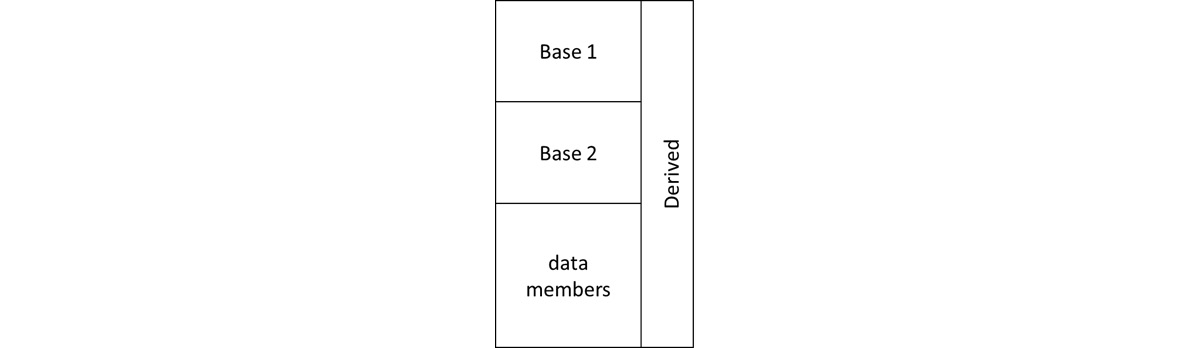
\includegraphics[keepaspectratio]{./image/Figure_1.1_B19262.jpg}
\caption{派生类的一种可能内存布局}
\label{fig1}
\end{figure}

从图 \ref{fig1} 可见,基类与派生类之间的指针转换通常涉及偏移计算。示例:

\begin{code}
// Example 01_cast.C
Derived d;
Derived* p = &d;
std::cout << "Derived: " << (void*)(p) <<
  " Base1: " << (void*)(static_cast<Base1*>(p)) <<
  " Base2: " << (void*)(static_cast<Base2*>(p)) <<
  std::endl;
\end{code}

程序输出类似:

\begin{code}
Derived: 0x7f97e550 Base1: 0x7f97e550 Base2: 0x7f97e560
\end{code}

可以看到 \texttt{Base1} 对象与 \texttt{Derived} 地址相同,而 \texttt{Base2} 有一个偏移(本例 16 字节)。看起来转换就是简单计算:如果你有一个 \texttt{Derived} 指针想转到 \texttt{Base2},加 16 即可。基类之间的偏移在编译期已知,编译器知道其布局。指针加偏移通常由硬件支持(现代 CPU 都支持),无需额外加法指令。似乎并不难。

那么如果指针是 \ci{null} 呢?指针值是 0。如果应用同样的“转换”,你得到 \texttt{16 (0x10)},此时你的空指针检查失效:

\begin{code}
void f(Base2* p) {
  if (p != nullptr) do_work(*p);
}
Derived* p = nullptr;
f(p); // 会尝试解引用 0x10 吗?
\end{code}

显然这很糟,所以我们可以假定 \ci{null} 保持为 \ci{null}。确实如此:

\begin{code}
Derived* p = nullptr;
std::cout << "Derived: " << (void*)(p) <<
  " Base1: " << (void*)(static_cast<Base1*>(p)) <<
  " Base2: " << (void*)(static_cast<Base2*>(p)) <<
  std::endl;
\end{code}

输出:

\begin{code}
Derived: 0x0 Base1: 0x0 Base2: 0x0
\end{code}

这是唯一可行的实现方式,但意味着一个从 \texttt{Derived*} 到 \texttt{Base*} 的简单隐式转换内部隐藏了一个对 \ci{null} 的条件分支。

另一种继承是 \textbf{private 继承}。私有继承时,派生类不会扩展基类的公共接口——基类方法在派生类中都变为私有。任何公共接口必须由派生类重新自定义(白纸起步)。并不假定派生类对象可以当作基类对象使用。派生类获得的是实现细节——可以使用基类的方法与数据成员实现自己的算法。因此常说 private 继承表达的是 \emph{has-a} 关系——派生对象内部包含一个基类实例。

私有继承后派生类与其基类的关系类似“类与其数据成员”的关系。后者实现技巧称为 \textbf{组合}(composition)——一个对象由任意数量的其它对象组成,后者作为数据成员。在没有特殊理由时应优先选择组合而非私有继承。那么什么时候用私有继承?有几种可能。第一,可以在派生类内用 \cii{using} 声明重新公开基类的某个 public 成员函数:

\begin{code}
class Container : private std::vector<int> {
  public:
  using std::vector<int>::size;
  ...
};
\end{code}

这在少数场景有用,但等价于一个内联转发函数:

\begin{code}
class Container {
  private:
  std::vector<int> v_;
  public:
  size_t size() const { return v_.size(); }
  ...
};
\end{code}

第二,可以在派生类成员函数内部把派生对象指针或引用转换为基类指针或引用;组合情况下等价于取数据成员地址。到此为止尚无充分理由使用私有继承,确实通常建议首选组合。但接下来两个理由更重要,任意一个都可能成为使用私有继承的动机。

其一与对象大小有关。常见存在“只提供方法、不含数据成员”的基类。此类没有自身数据,理应不占内存。但在 C++ 中它们必须拥有非零大小,这是因为语言要求任意两个不同对象/变量有不同唯一地址。通常若两个变量顺序声明,后者地址是前一个地址加上其大小:

\begin{code}
int x;     // 地址 0xffff0000,大小 4
int y;     // 地址 0xffff0004
\end{code}

为避免单独处理 0 大小对象,C++ 规定空对象大小为 1。如果这样的对象作为类的数据成员,它至少占 1 字节(后续成员的对齐可能增加此值)。这是浪费的内存,不会真正使用。而若空类作为基类使用,则没有要求其基类子对象必须有非零大小。整个派生对象必须非零,但派生对象地址、其第一个基类子对象地址以及其第一个数据成员地址都可以相同。因此 C++ 允许对空基类不分配额外内存,即使 \texttt{sizeof()} 对该类返回 1。虽然该“空基类优化”不是强制的,但大多数现代编译器都实现了:

\begin{code}
class Empty {
  public:
  void useful_function();
};
class Derived : private Empty {
  int i;
};    // sizeof(Derived) == 4
class Composed {
  int i;
  Empty e;
};    // sizeof(Composed) == 8
\end{code}

如果我们需要大量创建派生对象,节省的内存可能很可观。

第二个使用私有继承的理由与虚函数相关,下一节解释。

\section{多态与虚函数}

前面讨论 public 继承时我们提到,派生对象可以在任何需要基类对象的地方使用。虽然如此,很多时候我们仍希望知道对象的真实类型——即它被构造时的类型:

\begin{code}
Derived d;
Base& b = d;
...
b.some_method(); // b 实际上是 Derived 对象
\end{code}

\texttt{some\_method()} 属于 \texttt{Base} 公共接口,对 \texttt{Derived} 也必须有效。但在基类契约允许的灵活空间内,它可以“做不同的事情”。仍以鸟类层次为例:\texttt{FlyingBird} 可以假设存在一个 \texttt{fly()} 方法,所有从其派生的特定鸟类都必须支持飞行。但鹰与秃鹫的飞行方式不同,因此 \texttt{Eagle} 与 \texttt{Vulture} 中 \texttt{fly()} 的实现可以不同。对任意 \texttt{FlyingBird} 对象操作的代码可以调用 \texttt{fly()},而结果取决于对象真实类型。

该功能在 C++ 中由虚函数实现。虚的公共成员函数必须在基类中声明:

\begin{code}
class FlyingBird : public Bird {
  public:
  virtual void fly(double speed, double direction) {
    ... move the bird at the specified speed
        in the given direction ...
  }
  ...
};
\end{code}

派生类继承该函数的声明与实现。声明及其契约必须被遵守。如果该实现满足派生类需求则无需再做任何事;否则可以覆盖(override)基类实现:

\begin{code}
class Vulture : public FlyingBird {
  public:
  virtual void fly(double speed, double direction) {
    ... move the bird but accumulate
        exhaustion if too fast ...
  }
};
\end{code}

注意,派生类中覆盖基类虚函数时使用 \texttt{virtual} 关键字是可选的,没有语义影响(稍后会看到在某些风格中建议省略)。

调用虚函数时,C++ 运行时系统必须确定对象的真实类型。通常这一信息在编译期未知,只能在运行时判定:

\begin{code}
void hunt(FlyingBird& b) {
  b.fly(...);    // 可能是 Vulture 或 Eagle
  ...
};
Eagle e;
hunt(e);   // hunt() 内 b 实为 Eagle
           // 调用 FlyingBird::fly()
Vulture v;
hunt(v);   // b 实为 Vulture
           // 调用 Vulture::fly()
\end{code}

这种技术:一段代码操作一批基类对象并调用相同方法,而实际运行结果依对象真实类型而异,被称为 \textbf{运行时多态},支持该技术的对象被称为 \textbf{多态对象}。在 C++ 中,多态对象必须至少有一个虚函数,并且只有接口中通过虚函数实现(部分或全部实现)的部分才具备多态行为。

由此可知,虚函数声明与其覆盖实现必须一致——程序员在基类对象接口上调用函数,而实际运行的是派生类版本,仅当两者参数与返回类型一致时才可能。一个例外:若基类虚函数返回某类型的指针或引用,则覆盖允许返回该类型的派生类型的指针或引用(\textbf{协变返回类型})。

一个非常常见的多态层次特例是:基类没有一个“良好”默认实现。例如所有会飞的鸟都会飞,但它们的速度不同,没有理由在基类选一个速度作为默认。在 C++ 中我们可以拒绝在基类提供实现。

这样的函数称为 \textbf{纯虚函数}(pure virtual),包含纯虚函数的基类称为 \textbf{抽象类}:

\begin{code}
class FlyingBird {
  public:
  virtual void fly(...) = 0;     // 纯虚函数
};
\end{code}

抽象类只定义接口;由具体派生类实现。如果基类包含纯虚函数,程序中每个可被实例化的派生类都必须提供实现。换言之不能直接创建基类对象(派生类也可继续是抽象类,此时仍不能直接实例化,需再派生)。不过我们可以拥有指向基类对象的指针或引用——它们实际指向某个派生类型,但通过基类接口进行操作。

关于语法:覆盖虚函数时不必重复 \texttt{virtual}。若基类已经声明某名字与参数列表的虚函数,派生类同名同参函数自动为虚并覆盖基类。如果参数不同,则不会覆盖而是隐藏(shadow)基类同名函数,可能导致微妙 Bug:程序员意欲覆盖却没有正确匹配声明:

\begin{code}
class Eagle : public FlyingBird {
  public:
  void fly(int speed, double direction);
};
\end{code}

此处参数类型略有不同。\texttt{Eagle::fly()} 仍是虚的,但并未覆盖 \texttt{FlyingBird::fly()}。若后者为纯虚函数,编译器会因未实现而报错;若其有默认实现,则该 Bug 不会被编译器检测。C++11 提供 \texttt{override} 关键字帮助捕捉此类问题:

\begin{code}
class Eagle : public FlyingBird {
  public:
  void fly(int speed, double direction) override;
};
\end{code}

此时即使省略 \texttt{virtual} 也没关系;若 \texttt{FlyingBird} 中没有可被覆盖的虚函数,此代码无法编译。

也可以用 \texttt{final} 禁止进一步覆盖:

\begin{code}
class Eagle : public FlyingBird {
  public:
  // 所有 Eagle 飞行方式一致,BaldEagle / GoldenEagle 不能再改。
  void fly(int speed, double direction) final;
};
\end{code}

使用 \texttt{final} 很少见:很少设计要求完全禁止后续自定义。\texttt{final} 也可用于整个类,表示不可再派生,同样罕见。

那么覆盖时是否应再次写 \texttt{virtual}? 这是风格问题,但风格影响可读性与可维护性。推荐实践:

\begin{itemize}
\item 任何不覆盖基类函数的新虚函数必须写 \texttt{virtual}(包括无基类的类中的函数,以及派生类新增的虚函数)。
\item 其它覆盖函数不再写 \texttt{virtual},全部使用 \texttt{override}(例外:下一条)。
\item 最终覆盖(不允许再覆盖)使用 \texttt{final},且不再写 \texttt{override}。
\end{itemize}

这样有两点好处。其一:清晰——看到 \texttt{virtual} 就知道它不覆盖任何基类;看到 \texttt{override} 则必然是覆盖(否则不编译);看到 \texttt{final} 则同样是覆盖且是最后一次。其二:维护性——层次维护的大问题是“基类脆弱性”:你写了一组类,后来有人给基类函数加了一个参数,结果所有派生类函数不再覆盖,永远不被调用。始终使用 \texttt{override} 可以避免。

虚函数最常见的使用是结合 public 继承——由于每个派生对象也是基类对象(\emph{is-a}),程序可以把一组派生对象当作同类集合处理,而虚函数覆盖确保每个对象得到正确处理:

\begin{code}
void MakeLoudBoom(std::vector<FlyingBird*> birds)
  for (auto bird : birds) {
    bird->fly(...);   // 同一调用,结果不同
  }
}
\end{code}

但虚函数也可用于私有继承。用法不那么直观(且远少见)——毕竟私有继承的基类是“不可访问基类”(inaccessible base),尝试将派生指针转为基类失败。然而有一个上下文允许该转换:在派生类成员函数内部。以下展示如何让私有继承基类中的虚函数调用分派到派生:

\begin{code}
class Base {
  public:
  virtual void f() {
      std::cout << "Base::f()" << std::endl;
    }
  void g() { f(); }
};
class Derived : private Base {
  public:
  virtual void f() {
    std::cout << "Derived::f()" << std::endl;
  }
  void h() { g(); }
};
Derived d;
d.h(); // 输出 "Derived::f()"
\end{code}

\texttt{Base} 的公有方法在 \texttt{Derived} 中变为私有,因此我们不能直接调用。但可以在 \texttt{Derived} 的其它成员函数(如公有的 \texttt{h()})内部调用。我们当然可以直接在 \texttt{h()} 调用 \texttt{f()},但那无法证明任何事情——没人会惊讶 \texttt{Derived::h()} 调用 \texttt{Derived::f()}。

相反我们调用从 \texttt{Base} 继承的 \texttt{Base::g()}。在该函数内部我们处于 \texttt{Base} 上下文——其函数体可能在 \texttt{Derived} 实现前很久就写好、编译好。然而此处虚函数分派仍正常工作,调用 \texttt{Derived::f()},就像 public 继承一样。

上一节我们建议除非有理由,否则优先组合而非私有继承。这里的虚函数行为无法用组合轻易实现;若需要此行为,只能使用私有继承。

一个含虚函数的类必须在每个对象中编码其动态类型——这是在将指针转换为基类指针并丢失静态类型信息后在运行时知道对象真实类型的唯一手段。类型信息不是免费的:它占空间——多态对象总比相同数据成员但无虚函数的对象更大(通常多一个指针大小)。

额外大小与虚函数数量无关——只要有一个虚函数就需要类型信息。回想:基类指针可以转换为派生指针,但前提是我们知道正确的派生类型。使用 \cii{static_cast} 无法验证假设。对于非多态类(无虚函数),一旦丢失原始类型就无法恢复。但对多态对象,其类型编码在对象里,因此必须有办法利用该信息检查我们关于派生类型的假设是否成立。确实存在:\cii{dynamic_cast}:

\begin{code}
class Base { ... };
class Derived : public Base { ... };
Base* b1 = new Derived;     // 实际是 Derived
Base* b2 = new Base;   // 不是 Derived
Derived* d1 = dynamic_cast<Derived*>(b1);  // 成功
Derived* d2 = dynamic_cast<Derived*>(b2);  // d2 == nullptr
\end{code}

\cii{dynamic_cast} 不会告诉我们对象真实类型是什么;它让我们问一个问题——真实类型是 \texttt{Derived} 吗?如果猜对,转换成功并返回派生对象指针;否则返回 \ci{null}。\cii{dynamic_cast} 也能用于引用,差异仅在于——没有“空引用”:函数若返回引用必须指向有效对象,因此当请求类型不匹配真实类型时,只能抛出异常。

对性能敏感代码,需要关注 \cii{dynamic_cast} 的运行时成本。直觉可能认为虚函数调用与 \cii{dynamic_cast} 开销相近:两者都类似“这个 \texttt{Base} 指针其实是 \texttt{Derived} 吗?”的判定。简单基准表明并非如此:

\begin{code}
// Example 02_dynamic_cast.C
class Base {
  protected:
  int i = 0;
  public:
  virtual ~Base() {}
  virtual int f() { return ++i; }
};
class Derived : public Base {
  int f() override { return --i; }
};
Derived* p = new Derived;
// 测量 p->f() 的运行时间
// 测量 dynamic_cast<Derived*>(p) 的运行时间
\end{code}

基准可能显示(绝对值依硬件)虚调用约 1ns,而 \cii{dynamic_cast} 约 5~10ns。为何 \cii{dynamic_cast} 更贵?我们需要更多关于层次结构的背景(见下一节多重继承)。

\section{多重继承}

在 C++ 中,类可以同时从多个基类派生。回到鸟的例子:会飞的鸟彼此有很多共性,同时它们与其它会飞的动物(比如蝙蝠、昆虫)共享“飞行能力”。因飞行不限于鸟,我们可以把处理飞行的数据与算法抽离到独立基类。但鹰无疑也是一种鸟。若我们希望同时表达这两个关系,可以让 \texttt{Eagle} 继承两个基类:

\begin{code}
class Eagle : public Bird, public FlyingAnimal { ... };
\end{code}

此处两个继承均为 public,意味着派生类继承两个接口并需履行两份契约。若两个接口中都有同名方法会怎样?如果该方法不是虚的,则在派生类上调用会二义性而无法编译;如果该方法是虚的且派生类提供覆盖,则不再二义,因为调用派生实现。\texttt{Eagle} 现在既是 \texttt{Bird} 又是 \texttt{FlyingAnimal}:

\begin{code}
Eagle* e = new Eagle;
Bird* b = e;
FlyingAnimal* f = e;
\end{code}

两种向上转换都允许,反向转换需显式 static 或 dynamic cast。还有一个有趣转换——如果我们有一个 \texttt{FlyingAnimal} 指针,它同时也是一个 \texttt{Bird},能否从一个基转换到另一个基?可以,用 \cii{dynamic_cast}:

\begin{code}
Bird* b = new Eagle;   // 同时也是 FlyingAnimal
FlyingAnimal* f = dynamic_cast<FlyingAnimal*>(b);
\end{code}

在该上下文中 \cii{dynamic_cast}有时称为 \textbf{交叉转换}(\emph{cross-cast})——不是沿层次“向上/向下”而是“横向”在不同分支基类之间。

交叉转换也是 \cii{dynamic_cast}高成本的重要原因。虽然其最常用途是从 \texttt{Base*} 转到 \texttt{Derived*} 验证是否真是派生对象,但它也可能在同一派生对象的不同基之间转换。这是更难的问题。如果只是检查一个基对象是否真是某个特定派生类型,编译器此时知道 \texttt{Derived} 类型(\cii{dynamic_cast} 不能用于不完整类型),也就知道该派生的所有基类,检查是否其中之一很简单。但跨层次转换时,编译器仅知道两个基类:此时代码可能还不存在一个组合两者的派生类,它会在未来编写。编译器必须现在就生成正确代码:运行时遍历所有可能同时继承二者的派生类,判断当前对象是否其中之一(实际实现更高效,但目标相同)。

现实中这类开销通常不必要,因为大多数 \cii{dynamic_cast}确实只是做基到特定派生的判定。在很多场合这点开销无关紧要;但若需要更好性能,则没有办法让 \cii{dynamic_cast}更快。若想快速判断一个多态对象是否为给定类型,必须使用虚函数并(不幸地)维护一个所有可能类型(或感兴趣类型)的列表:

\begin{code}
enum type_t { typeBase, typeDerived1, typeDerived2 };
class Base {
  virtual type_t type() const { return typeBase; }
};
class Derived1 : public Base {
  type_t type() const override { return typeDerived1; }
};
鈥? // 省略其它派生
void process_derived1(Derived1* p);
void do_work(Base* p) {
  if (p->type() == typeDerived1) {
    process_derived1(static_cast<Derived1*>(p));
  }
}
\end{code}

多重继承在 C++ 中常被诟病。大量反对意见来自早期编译器对其实现差、效率低的年代。现代编译器下这已不再是主要顾虑。人们还说多重继承让层次更难理解与推理;更准确地说,设计一个良好且准确反映不同属性关系的多重继承层次更难,而糟糕的层次确实难以理解。

这些担忧主要适用于使用 public 继承的层次。多重继承也可以是私有的。相比单一私有继承,使用多重私有继承代替组合更加缺乏理由。不过空基类优化可以同时应用于多个空基类,若适用,仍是一个合理动机:

\begin{code}
class Empty1 {};
class Empty2 {};
class Derived : private Empty1, private Empty2 {
  int i;
};   // sizeof(Derived) == 4
class Composed {
  int i;
  Empty1 e1;
  Empty2 e2;
};   // sizeof(Composed) == 8
\end{code}

当派生类表示一个组合了多个互不重叠属性的系统时,多重继承尤其有效。后续本书在探讨各种设计模式及其 C++ 表示时会遇到这种情况。

\section{总结}

本章虽不是类与对象的完整指南或参考,但介绍并解释了理解本书其余章节示例所需的概念。我们的关注点在于用 C++ 表达设计模式,因此本章聚焦于正确使用类与继承,尤其注意通过哪些 C++ 特性表达不同组件之间的关系与交互——设计模式正是通过这些特性构建出的结构。

下一章将以类似方式介绍 C++ 模板相关知识,为理解后续章节奠定基础。

\section{问题}

\begin{itemize}
\item 对象在 C++ 中的重要性是什么?
\item public 继承表达什么关系?private 继承表达什么关系?什么是多态对象?
\item \cii{dynamic_cast}与 \cii{static_cast} 的区别是什么?为何 \cii{dynamic_cast}更昂贵?
\end{itemize}

\section{延伸阅读}

\begin{itemize}
\item \emph{Deciphering Object-Oriented Programming with C++}: \url{https://www.packtpub.com/product/deciphering-object-oriented-programming-with-c/9781804613900}
\item \emph{Software Architecture with C++}: \url{https://www.packtpub.com/product/software-architecture-with-c/9781838554590}
\item \emph{C++ Fundamentals}: \url{https://www.packtpub.com/product/c-fundamentals}
\item \emph{C++ Data Structures and Algorithms}:\url{ https://www.packtpub.com/product/c-data-structures-and-algorithm-design-principles}
\item \emph{Mastering C++ Programming}: \url{https://www.packtpub.com/product/mastering-c-programming}
\item \emph{Beginning C++ Programming}: \url{https://www.packtpub.com/product/beginning-c-programming}
\end{itemize}
%\chapter{An Introduction to Inheritance and Polymorphism}
%
%\textbf{C++} is, first and foremost, an object-oriented language, and objects are the fundamental building blocks of a C++ program. Class hierarchies are used to express relationships and interactions between different parts of a software system, define and implement interfaces between components, and organize data and code. While this isn't a book for teaching C++, the aim of this chapter is to give the reader enough knowledge about C++ language features as they relate to classes and inheritance, which will be used in later chapters. To that end, we won't attempt to completely describe the C++ tools for working with classes but introduce the concepts and language constructs that will be used throughout this book.
%
%The following topics will be covered in this chapter:
%
%\begin{itemize}
%\item
%  What are classes and what is their role in C++?
%\item
%  What are class hierarchies and how does C++ use inheritance?
%\item
%  What is runtime polymorphism and how is it used in C++?
%\end{itemize}
%
%\section{Classes and objects}
%
%Object-oriented programming is a way to structure a program by combining the algorithms and the data that the algorithms operate on into single entities called \textbf{objects}. Most object-oriented languages, including C++, are class-based. A \textbf{class} is a definition of an object---it describes the algorithms and the data, its format, and its relations to other classes. An object is a concrete instantiation of a class, that is, a variable. An object has an address, which is a location in memory. A class is a user-defined type. In general, any number of objects can be instantiated from the definition provided by the class (some classes limit the number of objects that can be created, but this is an exception, not the norm).
%
%In C++, the data contained in a class is organized as a collection of data members, or variables, of different types. The algorithms are implemented as functions---the methods of the class. While there's no language requirement that the data members of a class should be somehow relevant to the implementation of its methods, it's one of the signs of good design when the data is well encapsulated in the classes, and the methods have limited interaction with external data.
%
%This concept of \textbf{encapsulation} is central to the classes in C++---the language allows us to control which data members and methods are public---visible outside of the class, and which are internal---private to the class. A well-designed class has mostly, or only, private data members, and the only public methods are those needed to express the public interface of the class---in other words, what the class does. This public interface is like a contract---the class designer promises that this class provides certain features and operations. The private data and methods of the class are part of the implementation, and they can be changed as long as the public interface, the contract we've committed to, remains valid. For example, the following class represents a rational number and supports the increment operation, as exposed by its public interface:
%
%\begin{code}
%class Rational { public:
%  Rational& operator+=(const Rational& rhs);
%};
%\end{code}
%
%A well-designed class doesn't expose any more of the implementation details than it has to through its public interface. The implementation isn't part of the contract, although the documented interface may impose some restrictions on it. For example, if we promise that all rational numbers don't contain any common multipliers in the numerator and denomination, the addition should include the step of canceling them. That would be a good use of a private member function---the implementation of several other operations will need to call it, but the client of the class never needs to call it because every rational number is already reduced to its lowest terms before it's exposed to the callers:
%
%\begin{code}
%class Rational {
%  public:
%  Rational& operator+=(const Rational& rhs); private:
%  long n_; // numerator
%  long d_; // denominator
%  void  reduce();
%};
%Rational& Rational::operator+=(const Rational& rhs) {
%  n_ = n_*rhs.d_ + rhs.n_*d_;
%  d_ = d_*rhs.d_; reduce();
%  return *this;
%}
%Rational a, b; a += b;
%\end{code}
%
%The class methods have special access to the data members---they can access the private data of the class. Note the distinction between the class and the object here---\texttt{operator+=()} is a method of the \texttt{Rational} class and is invoked on the object, \texttt{a}. However, it has access to the private data of the \texttt{b} object as well, because \texttt{a} and \texttt{b} are objects of the same class. If a member function references a class member by name without any additional qualifiers, then it's accessing a member of the same class it's invoked on (we can make it explicit by writing \texttt{this-\textgreater{}n\_} and \texttt{this-\textgreater{}d\_}). Accessing members of another object of the same class requires a pointer or a reference to that object, but is otherwise not restricted, as would have been the case if we tried to access a private data member from a non-member function.
%
%By the way, C++ also supports C-style structs. But in C++, a struct isn't limited to just an aggregate of data members---it can have methods, public and private access modifiers, and anything else classes have. From a language point of view, the only difference between a class and a struct is the default access---in a class, all members and methods are private by default, while in a struct they're public. Beyond that, the use of structs instead of classes is a matter of convention---traditionally, structs are used for C-style structs (structs that would be legal in C) as well as \emph{almost} C-style structs, for example, a struct with only a constructor added. Of course, this boundary isn't precise and is a matter of coding styles and practices in each project or team.
%
%In addition to the methods and data members we've seen, C++ also supports static data and methods. A static method is very similar to a regular non-member function---it isn't invoked on any particular object, and the only way it can get access to an object of any type is through its arguments. However, unlike a non-member function, a static method retains its privileged access to the private data of the class.
%
%Classes by themselves are a useful way to group together (encapsulate) the algorithms and the data they operate on and to limit access to some data. However, the most powerful object-oriented features of C++ are inheritance and the resulting class hierarchies.
%
%\section{Inheritance and class hierarchies}
%
%Class hierarchies in C++ serve a dual purpose. On the one hand, they allow us to express relations between objects. On the other hand, they let us compose more complex types from simpler ones. Both uses are accomplished through inheritance.
%
%The concept of inheritance is central to the C++ use of classes and objects. Inheritance allows us to define new classes as extensions of existing ones. When a derived class is inherited from the base class, it contains, in some form, all of the data and the algorithms that were in the base class, and it adds some of its own. In C++, it's important to distinguish between two primary types of inheritance---public and private.
%
%Public inheritance inherits the public interface of the class. It also inherits the implementation---the data members of the base class are also a part of the derived class. But the inheritance of the interface is what distinguishes public inheritance---the derived class has, as a part of its public interface, the public member functions of the base class.
%
%Remember that the public interface is like a contract---we promise to the clients of the class that it supports certain operations, maintains some invariants, and obeys the specified restrictions. By publicly inheriting from the base class, we bind the derived class to the same contract (plus any extensions of the contract, should we decide to define additional public interfaces). Because the derived class also respects the interface contract of the base class, we could use a derived class in any place in the code where a base class is expected---we would not be able to use any of the extensions to the interface (the code expects the base class, we don't know about any extensions at that point), but the base class interface and its restrictions have to be valid.
%
%This is often expressed as the \emph{is-a principle}---an instance of a derived class is also an instance of the base class. However, the way we interpret the \emph{is-a} relationship in C++ isn't exactly intuitive. For example, is a square a rectangle? If it is, then we can derive the \texttt{Square} class from the \texttt{Rectangle} class:
%
%\begin{code}
%class Rectangle {
%  public:
%  double Length() const { return length_; }
%  double Width() const { return width_; }
%  ...
%  private:
%  double l_;
%  double w_;
%};
%class Square : public Rectangle {
%  ...
%};
%\end{code}
%
%Right away, there's something that doesn't seem right---the derived class has two data members for dimensions, but it really needs only one. We would have to somehow enforce that they're always the same. This doesn't seem so bad---the \texttt{Rectangle} class has the interface that allows for any positive values of length and width, and the \texttt{Square} imposes additional restrictions. But it's worse than that---the \texttt{Rectangle} class has a contract that allows the user to make the dimensions different. This can be quite explicit:
%
%\begin{code}
%class Rectangle {
%  public:
%  void Scale(double sl, double sw) {
%     // Scale the dimensions
%    length_ *= sl;
%    width_ *= sw;
%  }
%  ...
%};
%\end{code}
%
%Now, we have a public method that allows us to distort the rectangle, altering its aspect ratio. As with any other public method, it's inherited by the derived classes, so now the \texttt{Square} class has it too. In fact, by using public inheritance, we assert that a \texttt{Square} object can be used anywhere a \texttt{Rectangle} object is used, without even knowing that it's really a \texttt{Square}. Clearly, this is a promise we can't keep---when the client of our class hierarchy tries to change the aspect ratio of a square, we can't do it. We could ignore the call or report an error at runtime. Either way, we've violated the contract provided by the base class. There's only one solution---in C++, a square isn't a rectangle. Note that a rectangle is usually not a square, either---the contract provided by the \texttt{Square} interface could contain any number of guarantees that we can't maintain if we derive the \texttt{Rectangle} class from \texttt{Square}.
%
%Similarly, a penguin isn't a bird in C++ if the bird interface includes flying. The correct design for such cases usually includes a more abstract base class, \texttt{Bird}, that doesn't make any promises that at least one derived class can't keep (for example, a \texttt{Bird} object doesn't make a guarantee that it can fly). Then, we create intermediate-based classes, such as \texttt{FlyingBird} and \texttt{FlightlessBird}, that are derived from the common base class and serve as base classes for the more specific classes such as \texttt{Eagle} or \texttt{Penguin}. The important lesson here is that whether or not a penguin is a bird in C++ depends on how we define what a bird is, or, in C++ terms, what the public interface of the \texttt{Bird} class is.
%
%Because the public inheritance implies the \emph{is-a} relationship, the language allows a wide range of conversions between references and pointers to different classes in the same hierarchy. First of all, a conversion from a pointer to a derived class into a pointer to the base class is implicit (this is the same for references):
%
%\begin{code}
%class Base { ... };
%class Derived : public Base { ... };
%Derived* d = new Derived;
%Base* b = d;    // Implicit conversion
%\end{code}
%
%This conversion is always valid because an instance of the derived class is also an instance of the base class. The inverse conversion is possible but has to be made explicit:
%
%\begin{code}
%Base* b = new Derived;     // *b is really Derived
%Derived* d = b; // Does not compile, not implicit Derived*
%Derived* d1 =
%     static_cast<Derived*>(b);    // Explicit conversion
%\end{code}
%
%The reason this conversion isn't implicit is that it's valid only if the base class pointer really points to a derived object (otherwise, the behavior is undefined). The programmer, therefore, must explicitly assert, using the static cast, that somehow, through the logic of the program or a prior test or by some other means, it's known that this conversion is valid. If you aren't sure that the conversion is valid, there's a safer way to try it without causing undefined behavior; we'll learn about this in the next section.
%
%Note that the static (or implicit) conversion between pointers to base and derived classes is not quite as straightforward as you might think. The first base of any object always has the same address as the derived object itself, but then it gets more complicated. There is generally no standard requirement on the memory layout of derived classes with multiple bases:
%
%\begin{code}
%class Base1 { ... };
%class Base2 { ... };
%class Derived : public Base1, public Base2 { ... };
%\end{code}
%
%Most compilers will lay out the base classes first, then the data members of the derived class:
%
%\pandocbounded{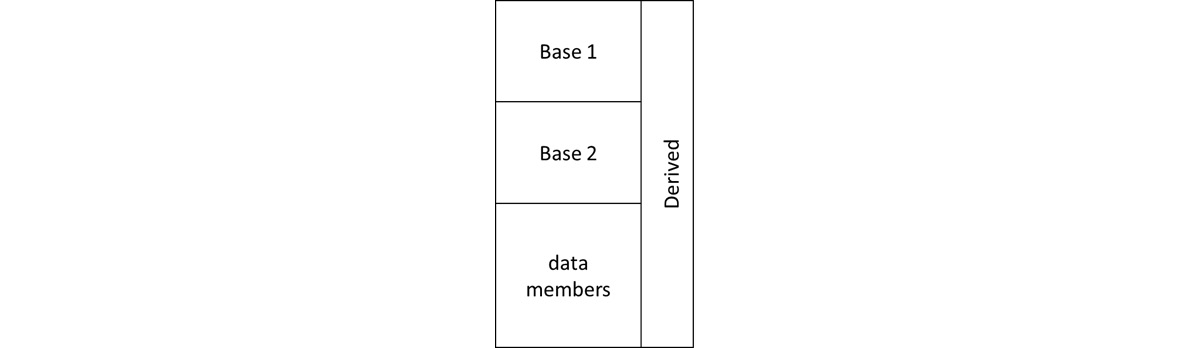
\includegraphics[keepaspectratio]{./image/Figure_1.1_B19262.jpg}}
%
%Figure 1.1 -- Possible memory layout of a derived class
%
%From \emph{Figure 1.1}, it is evident that pointer conversion between the base and derived classes generally involves offset calculations. We can easily see this in an example:
%
%\begin{code}
%// Example 01_cast.C
%Derived d;
%Derived* p = &d;
%std::cout << "Derived: " << (void*)(p) <<
%  " Base1: " << (void*)(static_cast<Base1*>(p)) <<
%  " Base2: " << (void*)(static_cast<Base2*>(p)) <<
%  std::endl;
%\end{code}
%
%The program prints something like this:
%
%\begin{code}
%Derived: 0x7f97e550 Base1: 0x7f97e550 Base2: 0x7f97e560
%\end{code}
%
%You can see that the \texttt{Base1} object is located at the same address as the \texttt{Derived} object, and \texttt{Base2} starts with an offset (16 bytes, in our case). Seems like the cast is an easy calculation: If you have a pointer to \texttt{Derived} and you want to cast to \texttt{Base2}, add 16. The offsets between base classes are known at compile time, and the compiler knows the layout it is using. Pointer offset calculations are usually implemented in hardware (all modern CPUs support them and do not require a separate addition instruction). This doesn't sound so hard at all.
%
%Now, what do you do if the pointer is \ci{null}? The pointer has a value of 0. If you apply the same \emph{conversion}, you get \texttt{16\ (0x10)}, and now your check for \ci{null} fails:
%
%\begin{code}
%void f(Base2* p) {
%  if (p != nullptr) do_work(*p);
%}
%Derived* p = nullptr;
%f(p); // Will it try to dereference 0x10?
%\end{code}
%
%Obviously, this would be very bad, so we can assume that \ci{null} pointers remain so. Indeed, they do:
%
%\begin{code}
%Derived* p = nullptr;
%std::cout << "Derived: " << (void*)(p) <<
%  " Base1: " << (void*)(static_cast<Base1*>(p)) <<
%  " Base2: " << (void*)(static_cast<Base2*>(p)) <<
%  std::endl;
%\end{code}
%
%This prints the same values for all pointers:
%
%\begin{code}
%Derived: 0x0 Base1: 0x0 Base2: 0x0
%\end{code}
%
%This is the only way to do casts, but it implies that a simple implicit cast from \texttt{Derived*} to \texttt{Base*} hides inside a conditional computation with a \ci{null} pointer check.
%
%The other kind of inheritance in C++ is \textbf{private inheritance}. When inheriting privately, the derived classes don't extend the public interface of the base class---all base class methods become private in the derived class. Any public interface has to be created by the derived class, starting from a clean slate. There's no assumption that an object of the derived class can be used in place of an object of the base class. What the derived class does get from the base class is the implementation details---both the methods and the data members can be used by the derived class to implement its own algorithms. It's said, therefore, that private inheritance implements a \emph{has-a} relationship---the derived object has an instance of the base class contained inside of it.
%
%The relation of the privately derived class to its base class is, therefore, similar to that of the relationship of a class to its data members. The latter implementation technique is known as \textbf{composition}---an object is composed of any number of other objects, which are all used as its data members. In the absence of any reason to do otherwise, the composition should be preferred to private inheritance. What, then, might be the reasons to use private inheritance? There are several possibilities. First of all, it's possible, within the derived class, to re-expose one of the public member functions of the base class with the help of a \texttt{using} declaration:
%
%\begin{code}
%class Container : private std::vector<int> {
%  public:
%  using std::vector<int>::size;
%  ...
%};
%\end{code}
%
%This can be useful in rare cases, but it's also equivalent to an inline forwarding function:
%
%\begin{code}
%class Container {
%  private:
%  std::vector<int> v_;
%  public:
%  size_t size() const { return v_.size(); }
%  ...
%};
%\end{code}
%
%Second, a pointer or reference to a derived object can be converted into a pointer or reference to the base object, but only inside a member function of the derived class. Again, the equivalent functionality for composition is provided by taking the address of a data member. So far, we haven't seen a good reason to use private inheritance, and indeed, the common advice is to prefer composition. But the next two reasons are more significant, and either one could be motivation enough to use private inheritance.
%
%One good reason to use private inheritance has to do with the size of the composed or derived objects. It isn't uncommon to have base classes that provide only methods but no data members. Such classes have no data of their own and, therefore, should not occupy any memory. But in C++, they have to be given a non-zero size. This has to do with the requirement that any two different objects or variables have different and unique addresses. Typically, if we have two variables declared one after the other, the address of the second one is the address of the first one, plus the size of the first one:
%
%\begin{code}
%int x;     // Created at address 0xffff0000, size is 4
%int y;     // Created at address 0xffff0004
%\end{code}
%
%To avoid the need to handle zero-sized objects differently, C++ assigns an empty object the size of one. If such an object is used as a data member of a class, it occupies at least 1 byte (the alignment requirements for the next data member may increase this value). This is wasted memory; it'll never be used for anything. On the other hand, if an empty class is used as a base class, there's no requirement that the base part of an object must have a non-zero size. The entire object of the derived class must have a non-zero size, but the address of a derived object, its base object, and its first data member can all be at the same address. Therefore, it's legal in C++ to allocate no memory for an empty base class, even though \texttt{sizeof()} returns 1 for this class. While legal, such empty base class optimization isn't required and is considered an optimization. Nonetheless, most modern compilers do this optimization:
%
%\begin{code}
%class Empty {
%  public:
%  void useful_function();
%};
%class Derived : private Empty {
%  int i;
%};    // sizeof(Derived) == 4
%class Composed {
%  int i;
%  Empty e;
%};    // sizeof(Composed) == 8
%\end{code}
%
%If we create many derived objects, the memory saved by the empty base optimization can be significant.
%
%The second reason to possibly use private inheritance has to do with virtual functions, and this will be explained in the next section.
%
%\section{Polymorphism and virtual functions}
%
%When we discussed public inheritance earlier, we mentioned that a derived object can be used in any place where a base object is expected. Even with this requirement, it's often useful to know what the actual type of the object is---in other words, what type the object was created as:
%
%\begin{code}
%Derived d;
%Base& b = d;
%...
%b.some_method(); // b is really a Derived object
%\end{code}
%
%\texttt{some\_method()} is a part of the public interface of the \texttt{Base} class and has to be valid for the \texttt{Derived} class as well. But, within the flexibility allowed by the contract of the base class interface, it can do something different. As an example, we've already used the avian hierarchy before to represent different birds, in particular, birds that can fly. The \texttt{FlyingBird} class can be assumed to have a \texttt{fly()} method, and every specific bird class derived from it has to support flight. But eagles fly differently from vultures, and so the implementation of the \texttt{fly()} method in the two derived classes, \texttt{Eagle} and \texttt{Vulture}, can be different. Any code that operates on arbitrary \texttt{FlyingBird} objects can call the \texttt{fly()} method, but the results will vary depending on the actual type of the object.
%
%This functionality is implemented in C++ using virtual functions. A virtual public function must be declared in the base class:
%
%\begin{code}
%class FlyingBird : public Bird {
%  public:
%  virtual void fly(double speed, double direction) {
%    ... move the bird at the specified speed
%        in the given direction ...
%  }
%  ...
%};
%\end{code}
%
%A derived class inherits both the declaration and the implementation of this function. The declaration and the contract it provides must be respected. If the implementation meets the needs of the derived class, there's no need to do anything more. But if the derived class needs to change the implementation, it can override the implementation of the base class:
%
%\begin{code}
%class Vulture : public FlyingBird {
%  public:
%  virtual void fly(double speed, double direction) {
%    ... move the bird but accumulate
%        exhaustion if too fast ...
%  }
%};
%\end{code}
%
%Note that the keyword \texttt{virtual}, when used in a derived class for methods that override base class virtual functions, is entirely optional and has no effect; we will see later that there are good reasons to omit that.
%
%When a virtual function is called, the C++ runtime system must determine what the real type of the object is. Usually, this information isn't known at compile time and must be determined at runtime:
%
%\begin{code}
%void hunt(FlyingBird& b) {
%  b.fly(...);    // Could be Vulture or Eagle
%  ...
%};
%Eagle e;
%hunt(e);   // Now b in hunt() is Eagle
%           // FlyingBird::fly() is called
%Vulture v;
%hunt(v);   // Now b in hunt() is Vulture
%           // Vulture::fly() is called
%\end{code}
%
%The programming technique where some code operates on any number of base objects and invokes the same methods, but the results depend on the actual type of these objects, is known as \textbf{runtime polymorphism}, and the objects that support this technique are \textbf{polymorphic}. In C++, polymorphic objects must have at least one virtual function, and only the parts of their interface that use virtual functions for some or all of the implementation are polymorphic.
%
%It should be evident from this explanation that the declaration of the virtual function and its overrides should be identical---the programmer calls the function on a base object, but the version that's implemented in the derived class runs instead. This can happen only if the two functions have identical arguments and return types. One exception is that if a virtual function in the base class returns a pointer or a reference to an object of some type, the override can return a pointer or a reference to an object derived from that type (this is known as \textbf{covariant} \textbf{return types}).
%
%A very common special case of polymorphic hierarchies is one where the base class doesn't have a good \emph{default} implementation of the virtual function. For example, all flying birds fly, but they all fly at different speeds, so there's no reason to select one speed as the default. In C++, we can refuse to provide any implementation for a virtual function in the base class.
%
%Such functions are called \textbf{pure virtual}, and any base class that contains a pure virtual function is known as an \textbf{abstract class}:
%
%\begin{code}
%class FlyingBird {
%  public:
%  virtual void fly(...) = 0;     // Pure virtual function
%};
%\end{code}
%
%An abstract class defines an interface only; it's the job of the concrete derived classes to implement it. If the base class contains a pure virtual function, every derived class that's instantiated in the program must provide an implementation. In other words, an object of a base class can't be created (a derived class could also be an abstract class, but then it cannot be instantiated directly either, we must derive another class from it). We can, however, have a pointer or a reference to an object of a base class---they really point to a derived class, but we can operate on it through the base class interface.
%
%A few notes on the C++ syntax---when overriding a virtual function, it isn't required to repeat the \texttt{virtual} keyword. If the base class declares a virtual function with the same name and arguments, the one in the derived class will always be a virtual function and will override the one from the base class. Note that, if the arguments differ, the derived class function doesn't override anything and instead shadows the name of the base class function. This can lead to subtle bugs where the programmer intended to override a base class function but didn't copy the declaration correctly:
%
%\begin{code}
%class Eagle : public FlyingBird {
%  public:
%  void fly(int speed, double direction);
%};
%\end{code}
%
%Here, the types of the arguments are slightly different. The \texttt{Eagle::fly()} function is also virtual, but it doesn't override \texttt{FlyingBird::fly()}. If the latter is a pure virtual function, the bug will be caught because every pure virtual function must be implemented in a derived class. But if \texttt{FlyingBird::fly()} has the default implementation, then the bug will go undetected by the compiler. C++11 provides a very useful feature that greatly simplifies finding such bugs---any function that's intended to be an override of a base class virtual function can be declared with the \texttt{override} keyword:
%
%\begin{code}
%class Eagle : public FlyingBird {
%  public:
%  void fly(int speed, double direction) override;
%};
%\end{code}
%
%The \texttt{virtual} keyword is still optional, but if the \texttt{FlyingBird} class doesn't have a virtual function that we could be overriding with this declaration, this code won't compile.
%
%It is also possible to prevent the derived classes from overriding a virtual function by declaring it \texttt{final}:
%
%\begin{code}
%class Eagle : public FlyingBird {
%  public:
%  // All Eagles fly the same way, derived classes BaldEagle
%  // and GoldenEagle cannot change this.
%  void fly(int speed, double direction) final;
%};
%\end{code}
%
%Note that the use of the \texttt{final} keyword is rare: it is unusual for the design to require that from this point on, the customizations should be disabled in the hierarchy. The \texttt{final} keyword can also be applied to the entire class: it means that no more classes can be derived from this one. Again, this is a rare situation.
%
%So, should or shouldn't you use the \texttt{virtual} keyword on overrides? This is a matter of style, but the style affects the readability and maintainability of the code. The following is the recommended practice:
%
%\begin{itemize}
%\item
%  Any virtual function that does not override one in the base class must use the \texttt{virtual} keyword. This includes both the functions in classes that have no bases and the functions added in derived classes.
%\item
%  Any other virtual function should not use the \texttt{virtual} keyword. All overrides should use the \texttt{override} keyword, with the following exception, which is also another rule.
%\item
%  A final override must use the \texttt{final} keyword and should not use the \texttt{override} keyword.
%\end{itemize}
%
%There are two advantages to this approach. The first is clarity and readability: if you see \texttt{virtual}, this is a virtual function that does not override anything. If you see \texttt{override}, this must be an override (otherwise the code would not compile). If you see \texttt{final}, this is also an override (again, the code would not compile otherwise) and it's the last such in the hierarchy. The second advantage shows up during code maintenance. One of the greatest problems with maintaining hierarchies is the base class fragility: you write a set of base and derived classes, someone else comes along and adds an argument to the base class function, and suddenly all your derived class functions don't override the base class ones and never get called. With consistent use of the \texttt{override} keyword, this will not happen.
%
%The most common use of virtual functions, by far, is in hierarchies that use public inheritance---since every derived object is also a base object (\emph{is-a} relationship), a program can often operate on a collection of derived objects as if they were all of the same types, and the virtual function overrides ensure that the right processing happens for every object:
%
%\begin{code}
%void MakeLoudBoom(std::vector<FlyingBird*> birds)
%  for (auto bird : birds) {
%    bird->fly(...);   // Same action, different results
%  }
%}
%\end{code}
%
%But virtual functions can also be used with private inheritance. The use is less straightforward (and much less common)---after all, an object that's derived privately can't be accessed through a base class pointer (a private base class is referred to as an \textbf{inaccessible base}, and an attempt to cast a derived class pointer to the base class will fail). However, there's one context in which this cast is permitted, and that's within a member function of the derived class. Here's, then, the way to arrange a virtual function call from a privately inherited base class to the derived one:
%
%\begin{code}
%class Base {
%  public:
%  virtual void f() {
%      std::cout << "Base::f()" << std::endl;
%    }
%  void g() { f(); }
%};
%class Derived : private Base {
%  public:
%  virtual void f() {
%    std::cout << "Derived::f()" << std::endl;
%  }
%  void h() { g(); }
%};
%Derived d;
%d.h(); // Prints "Derived::f()"
%\end{code}
%
%The public methods of the \texttt{Base} class become private in the \texttt{Derived} class, so we can't call them directly. We can, however, call them from another method of the \texttt{Derived} class, such as the public method \texttt{h()}. We can then call \texttt{f()} directly from \texttt{h()}, but that doesn't prove anything---it would come as no surprise if \texttt{Derived::h()} invoked \texttt{Derived::f()}.
%
%Instead, we call the \texttt{Base::g()} function that's inherited from the \texttt{Base} class. Inside that function, we're in the \texttt{Base} class---the body of this function may have been written and compiled long before the \texttt{Derived} class was implemented. And yet, in this context, the virtual function override works correctly and \texttt{Derived::f()} is called, just as it would if the inheritance were public.
%
%In the previous section, we recommended that composition is preferred to private inheritance unless there's a reason to do otherwise. There's no good way to implement similar functionality using composition; so, if the virtual function behavior is desired, private inheritance is the only way to go.
%
%A class with a virtual method has to have its type encoded into every object---this is the only way to know, at runtime, what was the type of the object when it was constructed, after we converted the pointer into a base class pointer and lost any other information about the original type. That type information isn't free; it takes space---a polymorphic object is always larger than an object with the same data members but no virtual methods (usually by the size of a pointer).
%
%The extra size doesn't depend on how many virtual functions the class has---at long as it has one, the type information must be encoded in the object. Now, recall that a pointer to the base class can be converted into a pointer to the derived class, but only if we know the correct type of the derived class. With the static cast, there's no way to test whether our knowledge is correct. For non-polymorphic classes (classes without any virtual functions), there can be no better way; once their original type is lost, there is no way to recover it. But for polymorphic objects, the type is encoded in the object, so there has to be a way to use that information to check whether our assumption is correct about which derived object this really is. Indeed, there is a way. It's provided by the dynamic cast:
%
%\begin{code}
%class Base { ... };
%class Derived : public Base { ... };
%Base* b1 = new Derived;     // Really Derived
%Base* b2 = new Base;   // Not Derived
%Derived* d1 = dynamic_cast<Derived*>(b1);  // Succeeds
%Derived* d2 = dynamic_cast<Derived*>(b2);  // d2 == nullptr
%\end{code}
%
%The dynamic cast doesn't tell us what the real type of the object is; rather, it allows us to ask the question---Is the real type \texttt{Derived}? If our guess at the type is correct, the cast succeeds and returns the pointer to the derived object. If the real type is something else, the cast fails and returns a \ci{null} pointer. The dynamic cast can also be used with references, with similar effects, save one---there's no \emph{null reference}. A function that returns a reference must always return a reference to some valid object. Since the dynamic cast can't return a reference to a valid object if the requested type doesn't match the actual type. The only alternative is to throw an exception.
%
%For performance-conscious code, it is important to be aware of the run-time cost of the dynamic cast. Naively, one might think that a virtual function call and a dynamic cast take about the same time: both boil down to the question -- is this pointer to \texttt{Base} really a pointer to \texttt{Derived}? A simple benchmark shows that this is not so:
%
%\begin{code}
%// Example 02_dynamic_cast.C
%class Base {
%  protected:
%  int i = 0;
%  public:
%  virtual ~Base() {}
%  virtual int f() { return ++i; }
%};
%class Derived : public Base {
%  int f() override { return --i; }
%};
%Derived* p = new Derived;
%// Measure the runtime of p->f();
%// Measure the runtime of dynamic_cast<Derived*>(p);
%\end{code}
%
%The benchmark results should look something like this (the absolute numbers will depend on the hardware): 1 nanosecond for the virtual call, and 5 to 10 nanoseconds for the dynamic cast. Why is the dynamic cast so expensive? We need to learn more about the hierarchies before we can answer this question.
%
%So far, we've limited ourselves to only one base class. While it's much easier to think about class hierarchies if we imagine them as trees, with the base class and the root and branches where multiple classes are derived from the same base, C++ doesn't impose such limitations. Next, we'll learn about inheriting from several base classes at once.
%
%\section{Multiple inheritance}
%
%In C++, a class can be derived from several base classes. Going back to our birds, let's make an observation---while flying birds have a lot in common with each other, they also have something in common with other flying animals, specifically, the ability to fly. Since flight isn't limited to birds, we may want to move the data and the algorithms related to processing flight into a separate base class. But there's also no denying that an eagle is a bird. We could express this relation if we used two base classes to construct the \texttt{Eagle} class:
%
%\begin{code}
%class Eagle : public Bird, public FlyingAnimal { ... };
%\end{code}
%
%In this case, the inheritance from both base classes is public, which means that the derived class inherits both interfaces and must fulfill two separate contracts. What happens if both interfaces define a method with the same name? If this method isn't virtual, then an attempt to invoke it on the derived class is ambiguous, and the program doesn't compile. If the method is virtual and the derived class has an override for it, then there's no ambiguity since the method of the derived class is called. Also, \texttt{Eagle} is now both \texttt{Bird} and \texttt{FlyingAnimal}:
%
%\begin{code}
%Eagle* e = new Eagle;
%Bird* b = e;
%FlyingAnimal* f = e;
%\end{code}
%
%Both conversions from the derived class into the base class pointer are allowed. The reverse conversions must be made explicitly using a static or a dynamic cast. There's another interesting conversion---if we have a pointer to a \texttt{FlyingAnimal} class that's also a \texttt{Bird} class, can we cast from one to the other? Yes, we can with a dynamic cast:
%
%\begin{code}
%Bird* b = new Eagle;   // Also a FlyingAnimal
%FlyingAnimal* f = dynamic_cast<FlyingAnimal*>(b);
%\end{code}
%
%When used in this context, the dynamic cast is sometimes called a \textbf{cross-cast}---we aren't casting up or down the hierarchy (between derived and based classes) but across the hierarchy---between the classes on different branches of the hierarchy tree.
%
%Cross-cast is also mostly responsible for the high runtime cost of the dynamic cast we have seen in the previous section. While the most common use of \texttt{dynamic\_cast} is to cast from \texttt{Base*} to \texttt{Derived*} to verify that a given object is really of the derived class, the cast could also be used to cast between bases of the same derived class. This is a much harder problem. If you just want to check that the base class object is really a derived one, the compiler knows the \texttt{Derived} type at this point (you cannot use the dynamic cast on incomplete types).
%
%Therefore, the compiler knows exactly what base classes this derived type has and can trivially check if yours is one of them. But when casting across the hierarchy, the compiler knows only two base classes: at the time when this code was written, a derived class that combines both may not exist, it will be written later. But the compiler must generate the correct code now. So, the compiler has to generate code that, at run time, digs through all the possible classes that are derived from both base classes to see if yours is one of them (the actual implementation is less straightforward and more efficient than that, but the task to be accomplished remains the same).
%
%In reality, this overhead is often unnecessary because, most of the time, the dynamic cast is indeed used to find out whether the base class pointer really points to a derived object. In many cases, the overhead is not significant. But if better performance is required, there is no way to make the dynamic cast faster. If you want a fast way to check whether a polymorphic object is really of a given type, you have to use virtual functions and, unfortunately, a list of all possible types (or at least all the ones you might be interested in):
%
%\begin{code}
%enum type_t { typeBase, typeDerived1, typeDerived2 };
%class Base {
%  virtual type_t type() const { return typeBase; }
%};
%class Derived1 : public Base {
%  type_t type() const override { return typeDerived1; }
%};
%鈥?
%void process_derived1(Derived1* p);
%void do_work(Base* p) {
%  if (p->type() == typeDerived1) {
%    process_derived1(static_cast<Derived1*>(p));
%  }
%}
%\end{code}
%
%Multiple inheritance is often maligned and disfavored in C++. Much of this advice is outdated and stems from the time when compilers implemented multiple inheritance poorly and inefficiently. Today, with modern compilers, this isn't a concern. It's often said that multiple inheritance makes the class hierarchy harder to understand and reason about. Perhaps it would be more accurate to say that it's harder to design a good multiple inheritance hierarchy that accurately reflects the relations between different properties, and that a poorly designed hierarchy is difficult to understand and reason about.
%
%These concerns mostly apply to hierarchies that use public inheritance. Multiple inheritance can be private as well. There's even less reason to use multiple private inheritance instead of composition than there was to use single private inheritance. However, the empty base optimization can be done on multiple empty base classes and remains a valid reason to use private inheritance, if it applies:
%
%\begin{code}
%class Empty1 {};
%class Empty2 {};
%class Derived : private Empty1, private Empty2 {
%  int i;
%};   // sizeof(Derived) == 4
%class Composed {
%  int i;
%  Empty1 e1;
%  Empty2 e2;
%};   // sizeof(Composed) == 8
%\end{code}
%
%Multiple inheritance can be particularly effective when the derived class represents a system that combines several unrelated, non-overlapping attributes. We'll encounter such cases throughout this book when we explore various design patterns and their C++ representations.
%
%\section{Summary}
%
%While by no means a complete guide or reference to classes and objects, this chapter introduced and explained the concepts you will need to understand the examples and explanations in the rest of this book. As our interest is and will be in representing design patterns in C++, this chapter focused on the proper use of classes and inheritance. We paid particular attention to what relations are expressed through different C++ features---it's through these features we'll express relations and interactions between different components that form a design pattern.
%
%The next chapter will similarly cover knowledge of C++ templates, which will be necessary to understand the subsequent chapters of this book.
%
%\section{Questions}
%
%\begin{itemize}
%\item
%  What is the importance of objects in C++?
%\item
%  Which relation is expressed by public inheritance? Which relation is expressed by private inheritance? What is a polymorphic object?
%\item
%  What is the difference between the dynamic cast and the static cast? Why is the dynamic cast so expensive?
%\end{itemize}
%
%\section{Further reading}
%
%\begin{itemize}
%\item
%  \emph{Deciphering Object-Oriented Programming with} \emph{C++}: https://www.packtpub.com/product/deciphering-object-oriented-programming-with-c/9781804613900
%\item
%  \emph{Software Architecture with} \emph{C++}: https://www.packtpub.com/product/software-architecture-with-c/9781838554590
%\item
%  \emph{C++} \emph{Fundamentals}: https://www.packtpub.com/product/c-fundamentals
%\item
%  \emph{C++ Data Structures and} \emph{Algorithms}: https://www.packtpub.com/product/c-data-structures-and-algorithm-design-principles
%\item
%  \emph{Mastering C++} \emph{Programming}: https://www.packtpub.com/product/mastering-c-programming
%\item
%  \emph{Beginning C++} \emph{Programming}: https://www.packtpub.com/product/beginning-c-programming
%\end{itemize}


% \chapter{Class and Function Templates}
\chapter{类与函数模板}

% The template programming features of C++ form a large and complex subject, with many books dedicated exclusively to teaching these features. In this book, we will use many of the advanced C++ generic programming features. How, then, should we prepare ourselves to understand these language constructs as they make their appearance throughout this book? This chapter takes an informal approach---instead of precise definitions, we demonstrate the use of templates through examples and explain what the different language features do. If you find your knowledge lacking at this point, you're encouraged to seek a deeper understanding and read one or more of the books dedicated entirely to the C++ language that are focused on explaining its syntax and semantics. Of course, if you wish for a more precise, formal description, you can refer to the C++ standard or a reference book.
本章要介绍的 C++ 模板编程特性是一个庞大而复杂的主题,已有许多专著专门系统讲解这些内容。本书后续会使用大量现代 C++ 泛型编程(模板)进阶特性。那么读者该如何准备,才能在后面的章节里理解这些语法结构的用法?本章采取一种“非正式”方式:我们不追求严密教科书式定义,而是通过示例展示模板的使用,并解释不同语言要素的作用。如果你发现自己当前理解还不够深入,建议补充阅读一到多本专门聚焦 C++ 语法与语义的权威教材;若需要更精确、形式化的描述,可以直接查阅 C++ 标准或参考手册。

% The following topics will be covered in this chapter:
本章将涵盖以下主题:

\begin{itemize}
% Templates in C++
\item C++ 中的模板
% Class and function templates
\item 类模板与函数模板
% Template instantiations
\item 模板实例化
% Template specializations
\item 模板特化(全特化与偏特化)
% Overloading of template functions
\item 模板函数的重载
% Variadic templates
\item 可变参数模板
% Lambda expressions
\item Lambda 表达式
% Concepts
\item Concepts(概念)
\end{itemize}

% \section{Templates in C++}
\section{C++ 中的模板}

% One of the greatest strengths of C++ is its support for generic programming. In generic programming, the algorithms and data structures are written in terms of generic types that will be specified later. This allows the programmer to implement a function or a class once, and later, instantiate it for many different types. Templates are a C++ feature that allows classes and functions to be defined on generic types. C++ supports three kinds of templates---function, class, and variable templates.
\cppsign{} 的一大核心优势在于其对“泛型编程”(\emph{generic programming})的强力支持。泛型编程的思想是:\emph{算法}与\emph{数据结构}以“之后才被具体化”的抽象类型来编写;这样我们只需实现一次函数或类,就能在稍后针对多种实际类型进行实例化生成代码。模板(\cii{template})正是 C++ 提供的机制,用来在“类型参数化”基础上定义类与函数。C++ 共支持三种模板:函数模板、类模板与变量模板。

% \subsection{Function templates}
\subsection{函数模板}

% Function templates are generic functions---unlike regular functions, a template function does not declare its argument types. Instead, the types are template parameters:
函数模板是一种“泛型函数”——不同于普通函数,它的参数类型不直接在形参列表里写死,而是通过模板形参(类型参数)来抽象:

\begin{code}
// Example 01
template <typename T>
T increment(T x) { return x + 1; }
\end{code}

% This template function can be used to increment a value of any type by one, for which adding one is a valid operation:
该模板函数可对“支持 +1 操作”的任意类型值做自增(返回新值):

\begin{code}
increment(5);    // T is int, returns 6
increment(4.2);  // T is double, return 5.2 
char c[10];
increment(c);    // T is char*, returns &c[1]
\end{code}

% Most template functions have some limitations on the types that are used as their template parameters. For example, our \cii{increment()} function requires that the expression \cii{x\ +\ 1} is valid for the type of \cii{x}. Otherwise, the attempt to instantiate the template will fail, with a somewhat verbose compilation error.
大多数函数模板对可用作模板参数的类型都存在某种“隐含前提”。例如这里的 \cii{increment()} 要求对类型 \cii{T} 的对象 \cii{x},表达式 \cii{x + 1} 必须可编译;否则实例化时会失败,并出现较为冗长的编译错误信息。

% Both non-member and class member functions can be function templates; however, virtual functions cannot be templates. The generic types can be used not only to declare function parameters but to declare any variables inside the body of the function:
自由函数与类成员函数都可以写成函数模板;但虚函数(virtual)不能是模板。模板类型参数不仅可用于形参,也可在函数体内部声明局部变量时使用:

\begin{code}
template <typename T> 
T sum(T from, T to, T step) {
  T res = from;
  while ((from += step) < to) { res += from; }
  return res;
}
\end{code}

% In C++20, simple template declarations can be abbreviated: instead of writing
C++20 中,某些简单形式的模板声明可以“省略写法”。例如下面的写法:

\begin{code}
template <typename T> void f(T t);
\end{code}

% we can write
可以简写为:

\begin{code}
// Example 01a
void f(auto t);
\end{code}

% Other than more terse declarations, there is no particular advantage to this abbreviation, and the feature is quite limited. First of all, \cii{auto} can be used only as the ``top-level'' parameter type; for example, this is invalid (but allowed by some compilers):
除语法更简短之外,此“缩写”并无其它额外优势,且适用范围有限。首先,\cii{auto} 只能出现在“顶层”形参类型位置;例如下面写法在标准里是非法的(尽管部分编译器可能放宽接受):

\begin{code}
void f(std::vector<auto>& v);
\end{code}

% and must still be written as
必须仍旧写成:

\begin{code}
template <typename T> void f(std::vector<T>& v);
\end{code}

% Also, if you need to use template type parameters elsewhere in the function declaration, you can't abbreviate them:
另外,如果你需要在函数声明的其它位置再次引用该模板类型参数,就不能使用这种缩写:

\begin{code}
template <typename T> T f(T t);
\end{code}

% Of course, you could declare the return type as \cii{auto} and use the trailing return type:
当然你可以把返回类型写成 \cii{auto},再用尾置返回类型:

\begin{code}
auto f(auto t) -> decltype(t);
\end{code}

% but at this point, the template is not really ``abbreviated.''
但这样做其实已经失去了“简写”的意义。

% We will see more of function templates later, but let's introduce class templates next.
后面还会继续深入函数模板,这里先转到类模板。

% \subsection{Class templates}
\subsection{类模板}

% Class templates are classes that use generic types, usually to declare their data members, but also to declare methods and local variables inside them:
类模板(class template)即“带有类型参数”的类定义。最常见地它用这些类型参数来声明数据成员,同时也可用于成员函数签名、返回值及内部局部变量声明:

\begin{code}
// Example 02
template <typename T> class ArrayOf2 {
  public:
  T& operator[](size_t i) { return a_[i]; }
  const T& operator[](size_t i) const { return a_[i]; }
  T sum() const { return a_[0] + a_[1]; }
  private:
  T a_[2];
};
\end{code}

% This class is implemented once, and can then be used to define an array of two elements of any type:
该类只需实现一次,随后即可用于构造任意类型的“两个元素的数组”对象:

\begin{code}
ArrayOf2<int> i; 
i[0] = 1; 
i[1] = 5;
std::cout << i.sum();                       // 6
ArrayOf2<double> x; 
x[0] = -3.5; 
x[1] = 4;
std::cout << x.sum();                       // 0.5
ArrayOf2<char*> c; 
char s[] = "Hello";
c[0] = s; 
c[1] = s + 2;
\end{code}

% Pay particular attention to the last example---you might expect the \cii{ArrayOf2} template not to be valid with a type such as \cii{char*}---after all, it has a method, \cii{sum()}, that does not compile if the type of \cii{a\_{[}0{]}} and \cii{a\_{[}1{]}} is a pointer. However, our example compiles as written---a method of a class template does not have to be valid until we try to use it. If we never call \cii{c.sum()}, then the fact that it would not compile never comes up, and the program remains valid. If we do call a member function that does not compile for the chosen template arguments, we get a syntax error in the body of the template (in our example, something about not being able to add two pointers). These error messages are rarely straightforward. Even if they were, it is unclear if the problem is in the body of the function, or if the function was not supposed to be called in the first place. Later in this chapter, we will see how to improve this situation.
请特别留意最后一个例子——你可能原本会认为 \cii{ArrayOf2} 不能用于 \cii{char*} 这样的类型:因为成员函数 \cii{sum()} 在元素是指针时无法编译(指针不能直接相加以得到语义化结果)。然而示例整体依然可以编译:原因在于“类模板的方法直到被实际用到才需要通过编译”。如果我们从不调用 \cii{c.sum()},就不会触发那段无效代码的实例化,程序整体仍合法。若调用了不适配实参类型的成员函数,则会在模板实例化阶段于函数体内部得到编译错误(例如“不能对两个指针做加法”)。此类错误信息往往不够直观,甚至让人不确定是实现写错,还是函数根本不该被调用。后文会介绍改进这一问题的手段。

\subsection{变量模板}
% The last kind of template in C++ is a variable template, which was introduced in C++14. This template allows us to define a variable with a generic type:
最后一种模板形式是“变量模板”(variable template),它在 \cpp[14] 中被引入。变量模板允许我们为“泛型类型”定义一个变量:

\begin{code}
// Example 03
template <typename T>
constexpr T pi = T(3.14159265358979323846264338327950288419716939937510582097494459230781L);
pi<float>;      // 3.141592
pi<double>;     // 3.141592653589793
\end{code}

% Variable templates are, for the most part, very straightforward to use, mostly for defining your own constants, but there are some interesting patterns that take advantage of them; we will see one in the next section.
变量模板总体使用非常直接,最常见用途是定义你自己的常量。不过也存在一些更有趣的用法模式;下一小节会看到一个例子。

\subsection{非类型模板参数}
% Usually, template parameters are types, but C++ also allows for several kinds of non-type parameters. First of all, template parameters can be values of integer or enumeration types:
通常模板参数是“类型”,但 \cppsign{} 也允许若干“非类型模板参数”(\emph{non-type template parameter})。首先,模板参数可以是\textbf{整数类型}或\textbf{枚举类型}的值:

\begin{code}
// Example 04
template <typename T, size_t N> 
class Array {
  public:
  T& operator[](size_t i) {
    if (i >= N) throw std::out_of_range("Bad index");
     return data_[i];
  }
  private:
  T data_[N];
};
Array<int, 5> a;      // OK
cin >> a[0];
Array<int, a[0]> b;   // Error
\end{code}

% This is a template with two parameters---the first is a type, but the second is not. It is a value of type \cii{size\_t} that determines the size of the array; the advantage of such a template over a built-in C-style array is that it can do range checking. The C++ standard library has a \cii{std::array} class template that should be used instead of implementing your own array in any real program, but it does make for an easy-to-follow example.
上面的模板有两个参数——第一个是类型,第二个则是“非类型”参数。第二个参数是一个 \cii{size_t} 常量,用来决定数组长度。与内置 C 风格数组相比,这种写法的优势是可以做越界检查。标准库已经提供了 \cii{std::array}(真实工程应优先使用),这里只是为了举例说明。

% The values of non-type parameters that are used to instantiate a template must be compile-time constants or \cii{constexpr} values---the last line in the preceding example is invalid because the value of \cii{a{[}0{]}} is not known until the program reads it in at runtime. C++20 allows floating-point and user-defined types for non-type template parameters; until then, the parameters were limited to integral types, pointers (including function and member pointers), references, and enumerations. Of course, the value of a non-type parameter has to be a compile-time constant so, for example, pointers to local variables are not allowed.
非类型模板参数用于实例化时所提供的值必须是“\emph{编译期常量}”或 \cii{constexpr} 值——示例里最后一行非法,就是因为 \cii{a[0]} 只有在运行期读取输入后才知道。\cpp[20] 起允许浮点数与用户自定义字面量类型作为非类型模板参数;在此之前仅限:\textbf{整型}、\textbf{指针}(\emph{含函数指针与成员指针})、\textbf{引用}、\textbf{枚举}。注意其值必须是编译期常量,因此指向局部变量的指针不能用作非类型模板实参。

% The numeric template parameters used to be very popular in C++ because they allow complex compile-time calculations to be implemented, but in the recent versions of the standard, \cii{constexpr} functions can be used to the same effect and are much easier to read. Of course, the standard takes with one hand and gives with the other, and so an interesting new use case emerged for non-template parameters combined with \cii{constexpr} functions: these functions, first introduced in C++11, are used to define ``immediate functions,'' or functions that are evaluated at compile time. The problem with \cii{constexpr} functions is that they \emph{may} evaluate at compile time but it's not required; they could also be evaluated at run time:
过去“数值型”非类型模板参数非常常见,因为它们能实现复杂的编译期计算。但后来标准引入并增强了 \cii{constexpr} 函数,可以达到类似目的且更易读。当然标准一手给一手也会再提供新能力——非类型模板参数与 \cii{constexpr} 结合出现了新的用例:在 C++11 中引入的 \cii{constexpr} 函数可用于定义“立即函数”(immediate function),即必须在编译期求值的函数。不过普通 \cii{constexpr} 函数只是“可以”在编译期执行,并非“必须”,也可能在运行期执行:

\begin{code}
constexpr size_t length(const char* s) {
  size_t res = 0;
  while (*(s++)) ++res;
  return res;
}
std::cout << length("abc") << std::endl;
char s[] = "runtime";
std::cout << length(s) << std::endl;
\end{code}

% Here we have a \cii{constexpr} function \cii{length()}. Does the length computation actually happen at compile time? There is no way to know short of examining the generated assembly code (which can differ from one compiler to another). The only way to be sure is to invoke the function in a compile-time context, for example:
我们定义了一个 \cii{constexpr} 函数 \cii{length()}。它的求值是否真的在编译期发生?除非去查看生成的汇编(而且不同编译器可能不同),否则无法保证。唯一能确定的方法是在“编译期上下文”中调用它,例如:

\begin{code}
static_assert(length("abc") == 3, ""); // OK
char s[] = "runtime";
static_assert(length(s) == 7, ""); // Fails
\end{code}

% The first assert compiles, and the second does not even though the value 7 is correct: the argument is not a compile-time value, so the evaluation must happen at run time.
第一个断言能通过;第二个虽然值也确实是 7,但却无法编译:原因是参数不是编译期常量,因此只能在运行期求值。

% In C++20, the function may be declared \cii{consteval} instead of \cii{constexpr}: this guarantees that the evaluation happens at compile time or not at all (thus, the second \cii{cout} statement in the preceding example will not compile). Prior to C++20, we have to get creative. Here is one way to enforce compile-time execution:
\cpp[20] 中可以把函数声明为 \cii{consteval}(替代 \cii{constexpr})以强制其“必须”在编译期求值,若无法则整体不成立(所以前面例子里第二个 \cii{cout} 将无法编译)。在 \cpp[20] 之前我们需要一些技巧。下面是强制编译期执行的一种方式:

\begin{code}
// Example 05c
template <auto V>
static constexpr auto force_consteval = V;
\end{code}

% The \cii{force\_consteval} variable template can be used to enforce compile-time evaluation as follows:
这个 \cii{force_consteval} 变量模板可以这样使用,从而迫使表达式在编译期被实例化与求值:

\begin{code}
std::cout << force_consteval<length("abc")> << std::endl;
char s[] = "runtime";
std::cout << force_consteval<length(s)> << std::endl;
\end{code}

% The second \cii{cout} statement does not compile because the function \cii{length()} cannot be evaluated as an immediate function. The variable template \cii{force\_consteval} uses a non-type template parameter whose type is not specified but deduced from the template argument (an \cii{auto} template parameter). This is a C++17 feature; in C++14 we have to use a rather unelegant macro to achieve the same result:
第二个 \cii{cout} 无法编译,因为 \cii{length()} 不能在该调用上下文被视为立即函数。这里的变量模板 \cii{force_consteval} 使用了一个“类型由模板实参自动推导”的非类型模板参数(即 \cii{auto} 模板参数),这是 \cpp[17] 特性;在 \cpp[14] 里需要借助不太优雅的宏才能模拟:

\begin{code}
// Example 05d
template <typename T, T V>
static constexpr auto force_consteval_helper = V;
#define force_consteval(V)
force_consteval_helper<decltype(V), (V)>
std::cout << force_consteval(length("abc")) << std::endl;
\end{code}

% If a non-type template parameter seems ``less than a type,'' you will like the next option, a parameter that is definitely more than a simple type.
如果觉得“非类型模板参数”看上去不够“高级”,那么你可能会喜欢下一类:其本身就是“模板”的模板参数。

\subsection{Template template parameters}
% The second kind of non-type template parameter worth mentioning is a \emph{template template} parameter---a template parameter that is itself a template. We will need them in the later chapters of this book. This template parameter is substituted---not with a name of a class, but a name of an entire template.
另一类值得关注的“高级”参数是 \textbf{模板模板参数}(template template parameter)——也就是“其自身是模板”的模板参数。后续多章会频繁用到。该参数被替换时,提供的不是一个具体类名,而是“一个模板”的名字。

% Here is a class template with a template template parameter:
下面是一个带模板模板参数的类模板示例:

\begin{code}
// Example 06a
template <typename T,
         template <typename> typename Container>
class Builder {
  Container<T> data_;
  public:
  void add(const T& t) { data_.push_back(t); }
  void print() const {
    for (const auto& x : data_) std::cout << x << " ";
    std::cout << std::endl;
  }
};
\end{code}

% The \cii{Builder} template declares a class that is used to construct (build) a container of an arbitrary type \cii{T}. The container itself does not have a specific type, it's a template itself.
\cii{Builder} 模板声明了一个类,用来“构建”由任意类型 \cii{T} 组成的容器。注意容器本身没有具体类型——它本身也是一个模板。

% It can be instantiated with any container template that takes one type argument:
它可以用“接收一个类型参数”的任意容器模板来实例化:

\begin{code}
template <typename T> class my_vector { ... };
Builder<int, my_vector> b;
b.add(1);
b.add(2);
b.print();
\end{code}

% Of course, there are additional requirements on the \cii{Container} template: it must have a single type parameter \cii{T} (the rest may be defaulted), it should be default-constructible, it must have a \cii{push\_back()} method, and so on. C++20 gives us a concise way to state these requirements and make them a part of the template interface; we will learn about it later in this chapter, in the \emph{Concepts} section.
当然,对 \cii{Container} 这个模板还隐含一些约束:它需要至少有一个类型参数(其余可有缺省),应支持默认构造,且需要有 \cii{push_back()} 等方法。\cpp[20] 提供了将这些“需求”直接写进接口的简洁方式——稍后在 \textbf{Concepts} 小节会学习。

% Here is a function template that has two template template parameters:
下面是一个拥有两个“模板模板参数”的函数模板:

\begin{code}
// Example 06b
template <template <typename> class Out_container,
          template <typename> class In_container,
          typename T> Out_container<T>
resequence(const In_container<T>& in_container) {
  Out_container<T> out_container;
  for (auto x : in_container) {
    out_container.push_back(x);
  }
  return out_container;
}
\end{code}

% This function takes an arbitrary container as an argument and returns another container, a different template, but instantiated on the same type, with the values copied from the input container:
这个函数接收任意容器参数,并返回另一个“不同模板类型”的容器,但两者都以相同元素类型实例化;返回容器中的元素值从输入容器复制而来:

\begin{code}
my_vector<int> v { 1, 2, 3, 4, 5 };
template <typename T> class my_deque { 鈥?};
auto d = resequence<my_deque>(v);// my_deque with 1 鈥?5
\end{code}

% Note that the compiler deduces both the type of the template argument (\cii{In\_container} as \cii{my\_vector}) and the type of its template parameter (\cii{T} as \cii{int}). Of course, the remaining template parameter \cii{Out\_container} cannot be deduced (it is not used in any parameters of the template function) and must be explicitly specified, which fits our intended use.
注意:编译器同时推导出了“输入容器模板”的类型(\cii{In_container = my_vector})以及其内部类型参数(\cii{T = int})。另一个模板参数 \cii{Out_container} 无法被推导(未出现在函数形参类型中),因此需要显式写出——这也正符合我们预期(调用端决定要转换成哪种容器模板)。

% There is a major limitation on template template parameters that is made more complex by the fact that different compilers enforce it unevenly (i.e., some compilers let through the code that should not compile but you would really like it to). The limitation is that the number of template parameters specified for the template template must match the number of the template parameters of the argument. Consider this template function:
模板模板参数有一个重要限制,并且不同编译器对其执行严格度不一致(有的会“放行”其实不符合标准的代码)。限制是:模板模板参数的“形参个数”必须与传入的“模板实参”的参数个数匹配。看下面的函数模板:

\begin{code}
template <template <typename> class Container, typename T>
void print(const Container<T>& container) {
  for (auto x : container) { std::cout << x << " "; }
  std::cout << std::endl;
}
std::vector<int> v { 1, 2, 3, 4, 5 };
print(v);
\end{code}

% This code may compile, but it depends on the version of the standard and the compiler's strict adherence to the standard: the \cii{std::vector} template has two template parameters, not one. The second parameter is the allocator; it has a default value, which is why we do not have to specify the allocator type when declaring a vector object. GCC, Clang, and MSVC all relax this requirement to some degree (but not to the same degree). Variadic templates, which we will see later in this chapter, offer another, more robust solution (at least in C++17 and later).
这段代码“可能”编译通过,取决于标准版本及编译器是否严格。\cii{std::vector} 实际有两个模板参数而非一个,第二个是分配器(有缺省参数),所以我们平时声明 vector 不必写出来。GCC / Clang / MSVC 在不同程度上放宽这一匹配要求。后面会介绍的“可变参数模板”提供了更健壮的解决方案(尤其在 C++17 及之后)。

% Templates are a kind of recipe for generating code. Next, we will see how we can convert these recipes into actual code we can run.
模板可以看作“生成代码的配方”。接下来我们来看:如何把这些“配方”在需要的时候转化为真正可执行的代码。

\section{模板实例化}
% The template name is not a type and cannot be used to declare a variable or call a function. To create a type or a function, the template must be instantiated. Most of the time, templates are instantiated implicitly when they are used. We will again start with function templates.
模板名字本身不是一个“类型”,因此不能直接用来声明变量或调用函数。要得到真正的类型或函数,必须对模板进行“实例化”(instantiation)。大多数情况下,模板在被“使用”时会被隐式实例化。我们再次从函数模板开始讨论。

\subsection{Function templates}
% To use a function template to generate a function, we have to specify which types should be used for all template type parameters. We can just specify the types directly:
要利用函数模板生成具体函数,必须为所有“类型模板参数”确定实际类型。可以显式地直接写出这些类型:

\begin{code}
template <typename T> T half(T x) { return x/2; }
int i = half<int>(5);
\end{code}

% This instantiates the \cii{half} function template with the \cii{int} type. The type is explicitly specified; we could call the function with an argument of another type, as long as it is convertible to the type we requested:
这会显式实例化出 \cii{half<int>}。虽然我们传入的参数类型也可以是别的,但需要能隐式转换成我们明确指定的那个类型:

\begin{code}
double x = half<double>(5);
\end{code}

% Even though the argument is an \cii{int}, the instantiation is that of \cii{half\textless{}double\textgreater{}}, and the return type is \cii{double}. The integer value \cii{5} is implicitly converted to \cii{double}.
尽管调用实参是 \cii{int},这里实例化的是 \cii{half<double>},返回类型为 \cii{double}。整数 \cii{5} 被隐式转换成 \cii{double}。

% Even though every function template can be instantiated by specifying all its type parameters, this is rarely done. Most of the uses of function templates involve the automatic deduction of types. Consider the following:
虽然可以总是显式列出全部类型参数来实例化函数模板,但实践中这样做并不常见。多数情况下会依赖“自动类型推导”。例如:

\begin{code}
auto x = half(8);    // int
auto y = half(1.5);    // double
\end{code}

% The template type can be deduced only from the template function arguments---the compiler will attempt to select the type for the \cii{T} parameter to match the type of the function argument that is declared with the same type. In our case, the function template has the argument \cii{x} of the \cii{T} type. Any call to this function has to provide some value for this argument, and this value must have a type. The compiler will deduce that \cii{T} must be that type. In the first call in the preceding code block, the argument is \cii{5}, and its type is \cii{int}. There is nothing better to do than to assume that \cii{T} should be \cii{int} in this particular template instantiation. Similarly, in the second call, we can deduce that \cii{T} must be \cii{double}.
模板形参类型的推导只能来自函数模板的形参类型——编译器会尝试让模板参数 \cii{T} 与对应函数形参类型一致。此处函数模板的参数 \cii{x} 声明为 \cii{T}。任意一次调用都会给该参数传一个“具有静态类型”的值,因此编译器可据此推得 \cii{T}。第一行调用中实参字面量 \cii{5} 的类型为 \cii{int},于是推导出实例化为 \cii{T=int}。第二次调用里字面量为浮点,推导出 \cii{T=double}。

% After this deduction, the compiler performs type substitution: all other mentions of the \cii{T} type are replaced by the type that was deduced; in our case, there is only one other use of \cii{T}, which is the return type.
完成推导后,编译器执行“类型替换”:将模板定义体内所有出现的 \cii{T} 都用推导出的具体类型替换;此例中另一个出现点是返回类型。

% Template argument deduction is widely used to capture types that we cannot easily determine:
模板实参推导广泛用于“捕获那些我们不想/不便显式写出的类型”:

\begin{code}
long x = ...;
unsigned int y = ...;
auto x = half(y + z);
\end{code}

% Here, we deduce the \cii{T} type to be whatever the type of the expression \cii{y\ +\ z} is (it's \cii{long}, but with template deduction, we don't need to specify that explicitly, and the deduced type will \emph{follow} the argument type if we ever change the types of \cii{y} and \cii{z}). Consider the following example:
这里我们让 \cii{T} 自动成为表达式 \cii{y + z} 的结果类型(这里是 \cii{long},但我们无需关心细节;如果以后改了 \cii{y} 或 \cii{z} 的类型,推导结果会自动“跟随变化”)。再看一个例子:

\begin{code}
template <typename U> auto f(U);
half(f(5));
\end{code}

% We deduce \cii{T} to match whatever type the \cii{f()} template function returns for an \cii{int} argument (of course, the definition of the \cii{f()} template function has to be provided before it can be called, but we do not need to dig into the header files where \cii{f()} is defined, as the compiler will deduce the right type for us).
这里我们令 \cii{T} 推导为 \cii{f(5)}(即 \cii{f()} 接收一个 \cii{int} 实参时)返回的类型。自然需要在此之前有 \cii{f()} 的定义可见,但我们不必去头文件里“手工查类型”,编译器会替我们完成推导。

% Only the types that are used to declare function arguments can be deduced. There is no rule that all template type parameters must be somehow present in the argument list, but any parameters that cannot be deduced must be explicitly specified:
只有出现在“函数形参类型”中的模板参数类型才能被推导。标准并不要求所有模板参数都必须出现在形参列表里;但是凡是无法推导出的参数,就必须显式指定:

\begin{code}
template <typename U, typename V> U half(V x) {
  return x/2;
}
auto y = half<double>(8);
\end{code}

% Here, the first template type parameter is explicitly specified, so \cii{U} is double, and \cii{V} is deduced to be \cii{int}.
此处第一个模板参数被显式指定为 \cii{double}(即 \cii{U}),而 \cii{V} 则由实参类型推导为 \cii{int}。

% Sometimes, the compiler cannot deduce template type parameters, even if they are used to declare arguments:
有时即便类型形参用于声明了函数参数,编译器也无法成功推导:

\begin{code}
template <typename T> T Max(T x, T y) {
  return (x > y) ? x : y;
}
auto x = Max(7L, 11); // Error
\end{code}

% Here, we can deduce from the first argument that \cii{T} must be \cii{long}, but from the second argument, we deduce that \cii{T} must be \cii{int}. It is often surprising to programmers who learn their way around templates that the \cii{long} type is not deduced in this case---after all, if we substitute \cii{long} for \cii{T} everywhere, the second argument will be implicitly converted, and the function will compile fine. So why isn't the \emph{larger} type deduced? Because the compiler does not attempt to find a type for which all argument conversions are possible: after all, there is usually more than one such type. In our example, \cii{T} could be \cii{double} or \cii{unsigned\ long}, and the function would still be valid. If a type can be deduced from more than one argument, the result of all these deductions must be the same.
这里从第一个实参可推得 \cii{T=long},但第二个实参又暗示 \cii{T=int}。初学者常疑惑:为什么编译器不选择“更大的” \cii{long}? —— 毕竟如果选 \cii{long},第二个参数还能隐式转换,函数也能工作。原因是:编译器不会“尝试寻找一个让所有实参都能转换过去”的公共类型,因为往往存在多种可能(此例也可用 \cii{double} 或 \cii{unsigned long})。当同一个模板参数从多个实参被推导时,所有推导结果必须一致,否则推导失败。

% Otherwise, the template instantiation is considered ambiguous.
如果不一致,则该次模板实例化“歧义”而失败。

% The type deduction is not always as straightforward as using the type of the argument for a type parameter. The argument may be declared with a type that's more complex than a type parameter itself:
类型推导并不总是“直接使用实参的静态类型”这么简单;形参类型往往比单独一个模板参数更复杂:

\begin{code}
template <typename T> T decrement(T* p) {
  return --(*p);
}
int i = 7;
decrement(&i);    // i == 6
\end{code}

% Here, the type of the argument is a \emph{pointer to} \cii{int}, but the type that is deduced for \cii{T} is \cii{int}. The deduction of types can be arbitrarily complex, as long as it's unambiguous:
此处实参类型是“指向 \cii{int} 的指针”,但推导出的 \cii{T} 是 \cii{int} 本身。推导逻辑只要不产生歧义,就可以相当复杂:

\begin{code}
template <typename T> T first(const std::vector<T>& v) {
  return v[0];
}
std::vector<int> v{11, 25, 67};
first(v);    // T is int, returns 11
\end{code}

% Here, the argument is an instantiation of another template, \cii{std::vector}, and we have to deduce the template parameter type from the type that was used to create this vector instantiation.
这里形参是另一个模板(\cii{std::vector})的实例化类型,我们需要从该实例化类型中再抽取出其内部模板参数类型。

% As we have seen, if a type can be deduced from more than one function argument, the result of these deductions must be the same. On the other hand, one argument can be used to deduce more than one type:
总结之前:如果某个模板类型形参可由多个实参推导,则所有推导结果必须一致。反过来,一个实参也可以同时为多个模板参数提供推导信息:

\begin{code}
template <typename U, typename V>
std::pair<V, U> swap12(const std::pair<U, V>& x) {
  return std::pair<V, U>(x.second, x.first);
}
swap12(std::make_pair(7, 4.2)); // pair of 4.2, 7
\end{code}

% Here, we deduce two types, \cii{U} and \cii{V}, from one argument, then use these two types to form a new type, \cii{std::pair\textless{}V,\ U\textgreater{}}. This example is unnecessarily verbose, and we can take advantage of a few more C++ features to make it both more compact and easier to maintain. First of all, the standard already has a function that deduces the argument types and uses them to declare a pair, and we have even used this function---\cii{std::make\_pair()}.
这里我们从单个实参同时推导出 \cii{U} 与 \cii{V},再组合成新的类型 \cii{std::pair<V, U>}。该写法有些啰嗦,可以借助更多 C++ 语言特性让其简化。首先,标准库已经提供了一个可推导实参类型并构造\ci{pair}的辅助函数 —— \cii{std::make_pair()}。

% Secondly, the return type of the function can be deduced from the expression in the \cii{return} statement (a C++14 feature). The rules of this deduction are similar to the rules of the template argument type deduction. With these simplifications, our example becomes the following:
其次,函数返回类型也可由 \cii{return} 语句中的表达式\emph{自动推导}(\cpp[14] 特性),其规则类似模板实参推导。于是例子可改写为:

\begin{code}
template <typename U, typename V>
auto swap12(const std::pair<U, V>& x) {
  return std::make_pair(x.second, x.first);
}
\end{code}

% Note that we don't explicitly use the types \cii{U} and \cii{V} anymore. We still need this function to be a template, since it operates on a generic type, that is, a pair of two types that we don't know until we instantiate the function. We could, however, use only one template parameter that would stand for the type of the argument:
注意现在我们不再显式使用 \cii{U} 与 \cii{V} 名字。函数依旧需要作为模板(其处理的类型依然是“未知的二元类型组合”)。不过我们甚至可以只用一个模板参数来代表整个实参类型:

\begin{code}
template <typename T> auto swap12(const T& x) {
  return std::make_pair(x.second, x.first);
}
\end{code}

% There is a significant difference between these two variants---the last function template will have its type deduced successfully from any call with one argument, no matter the type of that argument. If that argument is not \cii{std::pair}, or, more generally, if the argument is not a class or a struct or it does not have the \cii{first} and \cii{second} data members, the deduction will still succeed, but the type substitution will fail. On the other hand, the previous version will not even be considered for arguments that are not a pair of some types. For any \cii{std::pair} argument, the pair types are deduced, and the substitution should proceed without a problem. Can we use the last declaration and still restrict the type \cii{T} to be a pair or another class with a similar interface? Yes, and we will see several ways to do so later in this book.
这两种写法有重要区别——后一种(只用一个 \cii{T})面对任何单参数调用几乎都会“推导成功”;即使该实参并不是 \cii{std::pair}(更一般地:不是拥有 \cii{first}/\cii{second} 成员的数据结构),推导阶段仍会成功,但在替换使用这些成员时会编译失败。前一种写法则在“实参不是 pair”时根本不会进入候选。对于真正的 \cii{std::pair},前者能成功推导出两个类型并继续替换。如何在保持后一种简单声明的同时,限制 \cii{T} 必须是某种“具备 first/second 接口的类型”?答案是可以的,后续章节将介绍多种方式(如 Concepts 等)。

% Member function templates are very similar to non-member function templates, and their arguments are similarly deduced. Member function templates can be used in classes or class templates, which we will review next.
成员函数模板与非成员函数模板类似,其参数推导机制也一致。类或类模板中都可以定义成员函数模板,下面转到类模板继续。

\subsection{Class templates}
% Instantiation of class templates is similar to that of function templates---the use of a template to create a type implicitly instantiates the template. To use a class template, we need to specify the type arguments for the template parameters:
类模板的实例化方式与函数模板相似——当我们“用它来生成类型”时会触发隐式实例化。要使用类模板,必须为它的所有模板形参提供具体类型实参:

\begin{code}
template <typename N, typename D> class Ratio {
  public:
  Ratio() : num_(), denom_() {}
  Ratio(const N& num, const D& denom) :
    num_(num), denom_(denom) {}
  explicit operator double() const {
    return double(num_)/double(denom_);
  }
  private:
  N num_;
  D denom_;
};
Ratio<int, double> r;
\end{code}

% The definition of the \cii{r} variable implicitly instantiates the \cii{Ratio} class template for the \cii{int} and \cii{double} types. It also instantiates the default constructor of this class. The second constructor is not used in this code and is not instantiated. It is this feature of class templates---instantiating a template instantiates all data members, but does not instantiate the methods until they are used---that allows us to write class templates where only some of the methods compile for certain types. If we use the second constructor to initialize the values of \cii{Ratio}, then that constructor is instantiated, and must be valid for the given types:
对变量 \cii{r} 的定义会隐式实例化 \cii{Ratio<int,double>},并实例化其默认构造函数。第二个构造函数当前未被用到,因此暂未被实例化。类模板的这一特性——“实例化类模板时所有数据成员被实例化,但成员函数只有在被首次使用时才实例化”——使我们可以编写:某些成员仅在特定类型组合下才有效的模板。若我们接下来调用了第二个构造,那么它才会被实例化并要求对这些类型可编译:

\begin{code}
Ratio<int, double> r(5, 0.1);
\end{code}

% In C++17, these constructors can be used to deduce the types of the class template from the constructor arguments:
C++17 起可以利用构造函数实参推导类模板参数类型:

\begin{code}
Ratio r(5, 0.1);
\end{code}

% Of course, this works only if there are enough constructor arguments to deduce the types. For example, the default-constructed \cii{Ratio} object has to be instantiated with explicitly specified types; there is simply no other way to deduce them. Prior to C++17, a helper function template was often used to construct an object whose type can be deduced from the arguments. Similarly to \cii{std::make\_pair()}, which we looked at previously, we can implement a \cii{make\_ratio} function that will do the same thing as the C++17 constructor argument deduction:
当然,仅当“构造实参提供足够信息”时才可推导。比如默认构造的 \cii{Ratio} 对象就无法推导出模板参数,只能显式写类型。C++17 之前常用“辅助函数模板”来达成类似效果,类似我们之前见到的 \cii{std::make_pair()};可自定义 \cii{make_ratio} 来模拟 C++17 的构造实参推导:

\begin{code}
template <typename N, typename D>
Ratio<N, D> make_ratio(const N& num, const D& denom) {
  return { num, denom };
}
auto r(make_ratio(5, 0.1));
\end{code}

% The C++17 way of deducing template arguments should be preferred, if it is available: it does not require writing another function that essentially duplicates the class constructor, and does not make an additional call to the copy or move constructor to initialize the object (although in practice most compilers will perform return value optimization and optimize away the call to the copy or move constructor).
若可用,优先使用 C++17 的“类模板实参推导”机制:无需再写一个与构造逻辑重复的辅助函数,也避免潜在的额外复制/移动(尽管理论上 RVO 可能消除额外开销)。

% When a template is used to generate a type, it is instantiated implicitly. Both class and function templates can be explicitly instantiated as well. Doing so instantiates a template without using it:
模板被用来生成类型时是“隐式实例化”的;同时类和函数模板也可以“显式实例化”,即在未直接使用处强制生成对应实体:

\begin{code}
template class Ratio<long, long>;
template Ratio<long, long> make_ratio(const long&,
                                      const long&);
\end{code}

% Explicit instantiations are rarely needed, and will not be used elsewhere in this book.
显式实例化实际应用很少,本书其余地方不会再特意使用。

% While instantiations of class templates with specific template parameters behave (mostly) like regular classes, static data members of class templates deserve special mention. First, let us recall the common challenge of static class data members: they must be defined somewhere, and only once:
虽然带具体类型参数的类模板实例与普通类(大体)行为一致,但其“静态数据成员”有特殊注意点。先回顾普通类中 static 数据成员的常见问题:它们必须在某个翻译单元里且只出现一次定义:

\begin{code}
// In the header:
class A {
  static int n;
};
// In a C file:
int A::n = 0;
std::cout << A::n;
\end{code}

% Without such a definition, the program will not link: the name \cii{A::n} is not defined. But if the definition is moved into the header and the header is included in several compilation units, the program also will not link, this time the name \cii{A::n} is multiply defined.
若缺省该定义,会链接失败(未定义符号);若把定义写进头文件并被多个编译单元包含,又会因重复定义导致链接失败。

% The requirement to define static data members exactly once is not feasible for class templates: we need them defined for every set of template parameters the template is instantiated with, and we can't do that in any one compilation unit (other compilation units may instantiate the same template with different types). Fortunately, this is not necessary. Static members of class templates can (and should) be defined together with the template itself:
而对类模板来说“只定义一次”并不可行:不同翻译单元可能以不同类型实参实例化该模板,需要分别生成各自的静态成员。幸运的是标准允许:类模板的静态成员可以(也应当)直接在模板定义旁边提供定义:

\begin{code}
// In the header:
template <typename T> class A {
  static T n;
};
template <typename T> T A<T>::n {};
\end{code}

% While this technically results in multiple definitions, it is the job of the linker to consolidate them so we are left with a single definition (there is only one value of a static member variable for all objects of the same type).
这在技术上会在不同翻译单元产生多个“相同实体”的定义,链接器会做合并,保证针对“同一具体实例类型”只有一个静态变量实体。

% In C++17, inline variables offer a simpler solution:
C++17 引入的 inline 变量让写法更简单:

\begin{code}
// In the header:
template <typename T> class A {
  static inline T n {};
};
\end{code}

% This also works for non-template classes:
非模板类同样可以使用 inline 变量:

\begin{code}
// In the header:
class A {
  static inline int n = 0;
};
\end{code}

% If the static data member of a class template has a non-trivial constructor, this constructor is invoked once for every instantiation of this template (not for every object -- there is only one instance of a static member variable for all objects of the same type).
若静态数据成员具有非平凡构造函数,则每个“类模板实例”调用一次(而非每个对象一次),因为同一类型共享一份静态成员。

% Class templates, as we have used them so far, allow us to declare generic classes, that is, classes that can be instantiated with many different types. So far, all of these classes look exactly the same, except for the types, and generate the same code. This is not always desirable---different types may need to be handled somewhat differently.
目前为止的类模板都只是“把类型占位填进去”,生成的代码结构一致;但在某些场景,不同类型需要不同实现策略,这时需要“特化”。

% For example, let's say that we want to be able to represent not only a ratio of two numbers stored in the \cii{Ratio} object but also a ratio of two numbers stored elsewhere, with the \cii{Ratio} object containing pointers to these numbers. Clearly, some of the methods of the \cii{Ratio} object, such as the conversion operator to \cii{double}, need to be implemented differently if the object stores pointers to the numerator and denominator. In C++, this is accomplished by specializing the template, which we will do next.
例如:我们既想表示“内部保存两个值的比”,也想表示“指向外部两个值的比”(对象内部保存指针)。这时诸如转换为 \cii{double} 的运算符实现就应与原版不同。C++ 通过“模板特化(specialization)”来实现,我们马上展开。

\section{Template specializations}
% Template specializations allow us to make the generated template code differently for some types---not just the same code with different types substituted, but completely different code. There are two kinds of template specializations in C++---explicit, or full, specializations and partial specialization. Let's start with the former.
模板特化让我们可以针对特定类型“生成不同实现”的代码——不仅仅是把不同类型名替换进去,而是逻辑实现可完全不同。C++ 中有两类特化:显式(explicit / full)特化与偏特化(partial specialization)。先看显式特化。

\subsection{Explicit specialization}
% Explicit template specialization defines a special version of the template for a particular set of types. In an explicit specialization, all generic types are replaced by specific, concrete types. Since an explicit specialization is not a generic class or function, it does not need to be instantiated later. For the same reason, it is sometimes called \textbf{full specialization}. If the generic types are fully substituted, there is nothing generic left. An explicit specialization should not be confused with an explicit template instantiation---while both create an instantiation of a template for a given set of type arguments, an explicit instantiation creates an instantiation of the generic code, with the generic types substituted by the specific types. An explicit specialization creates an instantiation of the function or class with the same name but it overrides the implementation, so the resulting code can be completely different. An example should help us understand this distinction.
显式模板特化:为“特定一组类型”定义该模板的专门版本。在显式特化里,所有泛型类型都被具体类型取代,因此这段代码本身不再是“泛型”,也无需再后续实例化——故也称“全特化(full specialization)”。不要把“显式特化”与“显式实例化”混淆:二者都针对给定类型集合生成实体,但显式实例化只是对“原通用实现”做替换生成;显式特化则提供全新实现(覆盖原逻辑),可以完全不同。

% Let's start with a class template. Let's say that, if both the numerator and the denominator of \cii{Ratio} are \cii{double}, we want to compute the ratio and store it as a single number. The generic \cii{Ratio} code should remain the same, but for one particular set of types, we want the class to look entirely different. We can do this with an explicit specialization:
先从类模板看例子:如果 \cii{Ratio} 的分子和分母都是 \cii{double},希望直接计算结果并存成一个数;而对其他类型仍使用通用版本。这就可以用显式特化实现:

\begin{code}
template <> class Ratio<double, double> {
  public:
  Ratio() : value_() {}
  template <typename N, typename D>
    Ratio(const N& num, const D& denom) :
      value_(double(num)/double(denom)) {}
  explicit operator double() const { return value_; }
  private:
  double value_;
};
\end{code}

% Both template type parameters are specified to be \cii{double}. The class implementation is totally unlike the generic version---instead of two data members, we have just one; the conversion operator simply returns the value, and the constructor now computes the ratio of the numerator and the denominator. But it is not even the same constructor---instead of the non-template constructor \cii{Ratio(const\ double\&,\ const\ double\&)} that the generic version would have if it was instantiated for two \cii{double} template arguments, we provided a template constructor that can take two arguments of any types as long as they are convertible to \cii{double}.
两个模板参数都被指定为 \cii{double}。实现与通用版本完全不同:只保留一个存值成员;类型转换运算符直接返回该值;构造函数内部自行计算比值。并且这里提供的构造函数本身还是模板,可接收任意可转换为 \cii{double} 的类型参数(区别于通用版本中实例化后会得到的非模板构造 \cii{Ratio(const double&, const double&)})。

% Sometimes, we don't need to specialize the whole class template, because most of the generic code is still applicable. However, we may want to change the implementation of one or a few member functions. We can explicitly specialize the member function as well:
有时无需全特化整个类——大部分通用实现仍然适用,只想替换少数成员函数实现。这时可以“显式特化某个成员函数”本身:

\begin{code}
template <> Ratio<float, float>::operator double() const {
  return num_/denom_;
}
\end{code}

% Template functions can be explicitly specialized as well. Again, unlike an explicit instantiation, we get to write the body of the function, and we can implement it any way we want:
函数模板同样可以显式特化——与显式实例化不同,这里可重新写函数体,做完全自定义实现:

\begin{code}
template <typename T> T do_something(T x) {
  return ++x;
}
template <> double do_something<double>(double x) {
  return x/2;
}
do_something(3);        // 4
do_something(3.0);    // 1.5
\end{code}

% We cannot, however, change the number or the types of arguments or the return type---they must match the result of the substitution of the generic types, so the following does not compile:
但注意:不能改变参数个数、参数类型或返回类型——它们必须与“通用模板替换后”一致。所以下面这样会编译失败:

\begin{code}
template <> long do_something<int>(int x) { return x*x; }
\end{code}

% An explicit specialization must be declared before the first use of the template that would cause an implicit instantiation of the generic template for the same types. This makes sense---the implicit instantiation would create a class or a function with the same name and the same types as the explicit specialization. We would now have two versions of the same class or function in the program, and this violates the one definition rule and makes the program ill-formed (the exact rules can be found in the standard under \emph{{[}basic.def.odr{]}}).
显式特化必须在第一次会触发“对同一组类型进行隐式实例化”的使用之前声明。这是为了避免出现:隐式实例化生成的实体与显式特化生成的实体同名而导致 ODR(单一定义规则)违规。

% Explicit specializations are useful when we have one or a few types for which we need the template to behave very differently. However, this does not solve our problem with the ratio of pointers---we want a specialization that is still \emph{somewhat generic}, that is, it can handle pointers to any types, just not any other types. This is accomplished by a partial specialization, which we will look at next.
显式特化适合“极少数特定类型”需要完全不同实现的情形。但它无法满足“指针比”这种:既想限制为指针,又想对任意指针类型生效(仍保持一定泛型性)的需求——此时应使用“偏特化”,见下一小节。

\subsection{Partial specialization}
% Now, we are getting to the really interesting part of C++ template programming---partial template specializations. When a class template is partially specialized, it remains as generic code, but \emph{less generic} than the original template. The simplest form of a partial template is one where some of the generic types are replaced by concrete types, but other types remain generic:
下面来到 C++ 模板编程里非常有趣的部分:偏特化。类模板被“部分特化”后仍是泛型代码,但“比原版更窄一些”。最简单情形:只把部分模板参数换成具体类型,保留剩余依旧泛型:

\begin{code}
template <typename N, typename D> class Ratio {
  .....
};
template <typename D> class Ratio<double, D> {
  public:
  Ratio() : value_() {}
  Ratio(const double& num, const D& denom) :
    value_(num/double(denom)) {}
  explicit operator double() const { return value_; }
  private:
  double value_;
};
\end{code}

% Here, we convert \cii{Ratio} to a \cii{double} value if the numerator is \cii{double}, regardless of the denominator type. More than one partial specialization can be defined for the same template. For example, we can also specialize for the case when the denominator is \cii{double} and the numerator is anything:
此处:若分子为 \cii{double},无论分母是什么类型,都将其存为一个 \cii{double}。同一个模板可以有多个偏特化。例如再写一个“分母为 \cii{double}”的偏特化:

\begin{code}
template <typename N> class Ratio<N, double> {
  public:
  Ratio() : value_() {}
  Ratio(const N& num, const double& denom) :
    value_(double(num)/denom) {}
  explicit operator double() const { return value_; }
  private:
  double value_;
};
\end{code}

% When the template is instantiated, the best specialization for the given set of types is selected. In our case, if neither the numerator nor the denominator is \cii{double}, then the general template has to be instantiated---there are no other choices. If the numerator is \cii{double}, then the first partial specialization is a better (more specific) match than the general template. If the denominator is \cii{double}, then the second partial specialization is a better match. But what happens if both terms are \cii{double}? In this case, the two partial specializations are equivalent; neither is more specific than the other. This situation is considered ambiguous and the instantiation fails. Note that only this particular instantiation, \cii{Ratio\textless{}double,\ double\textgreater{}}, fails---it is not an error (at least, not a syntax error) to define both specializations, but it is an error to request an instantiation that cannot be uniquely resolved to the narrowest specialization. To allow any instantiation of our template, we have to remove this ambiguity, and the only way to do that is to provide an even more narrow specialization that would be preferred over the other two. In our case, there is only one option---a full specialization for \cii{Ratio\textless{}double,\ double\textgreater{}}:
实例化时编译器会选取“最匹配(最具体)”的特化:若分子/分母都不是 \cii{double},只能走通用模板;若分子为 \cii{double} 选第一个偏特化;若分母为 \cii{double} 选第二个。那两者都为 \cii{double} 呢?两偏特化同等具体,出现“二义性”导致实例化失败。注意:失败仅发生在 \cii{Ratio<double,double>} 这一次具体实例请求上;同时存在两个偏特化本身不是语法错误。要消除歧义,只能再提供一个“更具体”的全特化,使其优先级最高:

\begin{code}
template <> class Ratio<double, double> {
  public:
  Ratio() : value_() {}
  template <typename N, typename D>
    Ratio(const N& num, const D& denom) :
      value_(double(num)/double(denom)) {}
  explicit operator double() const { return value_; }
  private:
  double value_;
};
\end{code}

% Now, the fact that the partial specializations are ambiguous for the instantiation of \cii{Ratio\textless{}double,\ double\textgreater{}} is no longer relevant---we have a more specific version of the template than either of them, so that version is preferred over both.
这样偏特化之间的歧义被全特化“覆盖”,由全特化接管该实例。

% Partial specializations do not have to specify some of the generic types fully. Therefore, can keep all types generic, but impose some restrictions on them. For example, we still want a specialization where both the numerator and the denominator are pointers. They can be pointers to anything, so they are generic types, but \emph{less generic} than the arbitrary types of the general template:
偏特化不一定要把某个参数固定成具体类型,也可以“继续保持泛型”但加结构性约束。例如我们想要一个“分子与分母都是指针”的版本——指向任何类型都行,因此仍然泛型,但比“任意类型”更窄:

\begin{code}
template <typename N, typename D> class Ratio<N*, D*> {
  public:
  Ratio(N* num, D* denom) : num_(num), denom_(denom) {}
  explicit operator double() const {
    return double(*num_)/double(*denom_);
  }
  private:
  N* const num_;
  D* const denom_;
};
int i = 5; double x = 10;
auto r(make_ratio(&i, &x));        // Ratio<int*, double*>
double(r);                    // 0.5
x = 2.5;
double(r);                    // 2
\end{code}

% This partial specialization still has two generic types, but they are both pointer types, \cii{N*} and \cii{D*}, for any \cii{N} and \cii{D} types. The implementation is totally unlike that of the general template. When instantiated with two pointer types, the partial specialization is \emph{more specific} than the general template and is considered a better match. Note that, in our example, the denominator is \cii{double}. So why isn't a partial specialization for the \cii{double} denominator considered? That is because, while the denominator is \cii{double} as far as the program logic is concerned, technically it is \cii{double*}, a completely different type, and we do not have a specialization for that.
此偏特化仍有两个泛型参数,但形式为指针类型 \cii{N*}、\cii{D*}。实现与通用模板完全不同。实例化时若模板实参是两个指针类型,该偏特化比通用模板“更具体”被优先选中。注意例子里分母变量逻辑上引用的是一个 \cii{double} 值,但类型却是 \cii{double*}(指针);我们并没有“分母为 double(非指针)”的特化,所以不会与之前的偏特化冲突。

% To define a specialization, a general template must first be declared. It does not, however, need to be defined---it is possible to specialize a template that does not exist in the general case. To do so, we must forward-declare the general template, then define all the specializations we need:
要编写一个特化,首先需要“声明”原始模板(可以不提供定义)。也就是说允许“只有特化,没有通用定义”——做法是先前向声明,再给出所有需要的(偏)特化:

\begin{code}
template <typename T> class Value; // Declaration 
template <typename T> class Value<T*> {
  public:
  explicit Value(T* p) : v_(*p) {} private:
  T v_;
};
template <typename T> class Value<T&> {
  public:
  explicit Value(T& p) : v_(p) {}
  private:
  T v_;
};
int i = 5; int* p = &i; int& r = i;
Value<int*> v1(p); // T* specialization
Value<int&> v2(r); // T& specialization
\end{code}

% Here, we have no general \cii{Value} template, but we have partial specializations for any pointer or reference types. If we try to instantiate the template on some other type, like \cii{int}, we will get an error stating that the \cii{Value\textless{}int\textgreater{}} type is incomplete---this is no different than trying to define an object with only a forward declaration of the class.
此处没有通用 \cii{Value} 定义,只有指针与引用两种偏特化。若尝试实例化 \cii{Value<int>} 会报“类型不完全”错误,与只前向声明一个类就定义对象同样违规。

% So far, we have seen only examples of partial specializations for class templates. Unlike the earlier discussion of full specializations, we have not seen a single function specialization here. There is a very good reason for that---a partial function template specialization does not exist in C++. What is sometimes incorrectly called a partial specialization is nothing more than overloading template functions. On the other hand, overloading template functions can get quite complex and is worth learning about---we will cover this next.
目前展示的偏特化示例都针对“类模板”。函数模板不存在“偏特化”这一语言机制——常被误称为“偏特化”的,其实是“函数模板重载”。函数模板重载规则更复杂,下一节详述。

\subsection{Template function overloading}
% We are used to regular functions, or class methods, being overloaded---multiple functions with the same name have different parameter types. Each call invokes the function with the best match of the parameter types to the call arguments, as shown in the following example:
我们熟悉普通函数或成员函数的“重载”——同名函数通过不同的参数类型区分。调用时编译器挑选形参与实参“最佳匹配”的那个,如下:

\begin{code}
// Example 07
void whatami(int x) {
  std::cout << x << " is int" << std::endl;
}
void whatami(long x) {
  std::cout << x << " is long" << std::endl;
}
whatami(5);    // 5 is int
whatami(5.0);    // Compilation error
\end{code}

% If the arguments are a perfect match for one of the overloaded functions with the given name, that function is called. Otherwise, the compiler considers conversions to the parameter types of the available functions. If one of the functions offers \emph{better} conversions, that function is selected. Otherwise, the call is ambiguous, just as in the last line of the preceding example. The precise definition of what constitutes the \emph{best} conversion can be found in the standard (see the section \emph{Overloading}, more specifically, subsection \emph{{[}over.match{]}}). Generally, the \emph{cheapest} conversions are the ones such as adding \cii{const} or removing a reference; then, there are conversions between built-in types, conversions from derived to base class pointers, and so on. In the case of multiple arguments, each argument for the chosen function must have the best conversion. There is no \emph{voting}---if a function has three arguments, and two are an exact match for the first overload, while the third one is an exact match for the second overload, then even if the remaining arguments are implicitly convertible to their corresponding parameter types, the overloaded call is ambiguous.
若某个重载与实参完全匹配,就直接使用它;否则编译器考虑各候选所需的隐式转换,并挑选拥有“更好转换序列”的函数。如果不存在唯一最佳,则调用“二义”。“最佳转换”定义见标准 Overloading/[over.match]。通常“代价最低”如添加 const、去掉引用 优先;之后是内建类型之间、派生到基类指针等。多参数时,被选函数对“每个”实参都需是最佳;不存在“投票机制”。

% The presence of templates makes the overload resolution much more complex. Multiple function templates with the same name and, possibly, the same number of arguments, can be defined, in addition to non-template functions. All of these functions are the candidates for an overloaded function call, but the function templates can generate functions with different parameter types, so how do we decide what the actual overloaded functions are? The exact rules are even more complex than the ones for non-template functions, but the basic idea is this---if there is a non-template function that is a near-perfect match to the call arguments, that function is selected. The standard, of course, uses much more precise terms than \emph{near-perfect}, but \emph{trivial} conversions, such as adding \cii{const}, fall under that category---you get them \emph{at no cost}. If there is no such function, the compiler will attempt to instantiate all function templates with the same name to a near-perfect match, using the template argument deduction. If exactly one of the templates was instantiated, the function created by this instantiation is called. Otherwise, overload resolution continues the usual way among the non-template functions.
模板引入后重载决议更复杂:同名可存在多个函数模板与普通函数。函数模板经推导实例化后才加入候选。规则概要:若存在“非模板”近乎完美匹配(只需微小转换),直接选它;否则尝试对所有同名模板做类型推导,能得到“近似完美匹配”实例的模板加入候选,且只有唯一一个时就选它,否则继续与其它候选比较。

% This is a very simplified description of a very complex process, but there are two important points---firstly, if there is an equally good match of a call to a template and a non-template function, the non-template function is preferred, and secondly, the compiler does not attempt to instantiate the function templates into something that might be convertible to the types we need. The template functions must match the call almost perfectly after the argument type deduction, or they are not called at all. Let's add a template to our previous example:
总结:1) 模板与非模板同样匹配时优先非模板;2) 不会“为可能通过转换匹配”而实例化模板——推导后需要几乎完美匹配。添加一个模板重载:

\begin{code}
void whatami(int x); // Same as above
void whatami(long x); // Same as above
template <typename T> void whatami(T* x) {
  std::cout << x << " is a pointer" << std::endl;
}
int i = 5;
whatami(i);    // 5 is int
whatami(&i);    // 0x???? is a pointer
\end{code}

% Here, we have what looks like a partial specialization of a function template. But it really isn't---it is just a function template---there is no general template for which it could be a specialization. Instead, it is simply a function template whose type parameter is deduced from the same arguments, but using different rules. The template can have its type deduced if the argument is a pointer of any kind. This includes a pointer to \cii{const}---\cii{T} could be a \cii{const} type, so if we call \cii{whatami(ptr)}, where \cii{ptr} is \cii{const\ int*}, that first template overload is a perfect match when \cii{T} is \cii{const\ int}. If the deduction succeeds, the function generated by the template, that is, the template instantiation, is added to the overload set.
这个模板看似“偏特化”,其实只是普通函数模板。只要实参是任意指针(包括指向 const),即可推导。例如传 \cii{const int*} 时推导 \cii{T=const int},该实例加入候选。

% For the \cii{int*} argument, it is the only overload that works, so it is called. But what happens if more than one function template can match the call, and both instantiations are valid overloads? Let's add one more template:
当实参为 \cii{int*} 时只有该模板适用。再添加一个更泛的重载看看冲突:

\begin{code}
void whatami(int x); // Same as above
void whatami(long x); // Same as above
template <typename T> void whatami(T* x); // Same as above
template <typename T> void whatami(T&& x) {
  std::cout << "Something weird" << std::endl;
}
class C {    };
C c;
whatami(c);    // Something weird
whatami(&c);    // 0x???? is a pointer
\end{code}

% This template function accepts its arguments by the universal reference, so it can be instantiated for any call to \cii{whatami()} with one argument. The first call, \cii{whatami(c)}, is easy---the last overload, with \cii{T\&\&}, is the only one that can be called. There are no conversions from \cii{c} to a pointer or an integer. But the second call is tricky---we have not one, but two template instantiations that are a perfect match for the call, with no conversions needed. So why is this not an ambiguous overload? Because the rules for resolving overloaded function templates are different than the rules for non-template functions and resemble the rules for selecting the partial specialization of a class template (which is another reason why function template overloads are often confused with partial specializations). The template that is more specific is a better match.
新增 \cii{T&&} 重载(转发引用)可以匹配任意单参数调用。第一次调用只有它适用;第二次调用与“指针参数版本”同时完美匹配,却不二义,因为规则优先更具体(仅接受指针)的模板。

% In our case, the first template is more specific---it can accept any pointer argument, but only pointers. The second template can accept any argument at all, so any time the first template is a possible match, the second is too, but not the reverse. If a more specific template can be used to instantiate a function that is a valid overload, then this template is used.
“指针版本”更具体:只接受指针;\cii{T&&} 更泛,涵盖所有情况。若具体模板适用则用它,否则回退。

% Otherwise, we have to fall back to the more general template.
若不适用则退回更泛模板。

% The very general template functions in the overload set sometimes lead to unexpected results. Let's say we have the following three overloads for \cii{int}, \cii{double}, and anything:
过度泛化的模板可能导致意外结果。设有对 int、double 及“任意类型”三个重载:

\begin{code}
void whatami(int x) {
  std::cout << x << " is int" << std::endl;
}
void whatami(double x) {
  std::cout << x << " is double" << std::endl;
}
template <typename T> void whatami(T&& x) {
  std::cout << "Something weird" << std::endl;
}
int i = 5;
float x = 4.2;
whatami(i);    // i is int
whatami(x);    // Something weird
whatami(1.2);    // 1.2 is double
\end{code}

% The first call has an \cii{int} argument, so \cii{whatami(int)} is a perfect match. The second call would have gone to \cii{whatami(double)} if we did not have the template overload---the conversion from \cii{float} to \cii{double} is implicit (so is the conversion from \cii{float} to \cii{int}, but the conversion to \cii{double} is preferred). But it's still a conversion, so when the function template instantiates to a perfect match of \cii{whatami(float\&\&)}, that is the best match and the chosen overload. The last call has a \cii{double} argument, and again we have a perfect match to a non-template function \cii{whatami(double)}, so it is preferred over any alternative.
第一次调用选 \cii{whatami(int)};第二次若无模板会选 double 版本,但有了模板得到完美匹配 \cii{whatami(float&&)},无需转换而胜出;第三次 double 直接匹配非模板重载。

% It should be noted that overloading pass-by-value and pass-by-reference functions for the same parameter types often creates ambiguities in overload resolution. For example, these two functions are almost always ambiguous:
针对同一模式同时提供“万能引用”和“值传递”版本极易造成二义:

\begin{code}
template <typename T> void whatami(T&& x) {
  std::cout << "Something weird" << std::endl;
}
template <typename T> void whatami(T x) {
  std::cout << "Something copyable" << std::endl;
}
class C {};
C c;
whatami(c);
\end{code}

% As long as the argument to the function can be copied (and our object \cii{c} is copyable), the overload is ambiguous and the call will not compile. The problem does not happen when a more specific function overloads a more general one (in all our previous examples, \cii{whatami(int)} used pass-by-value with no problems), but mixing the two types of parameter passing for similarly general functions is inadvisable.
只要参数可复制,上述调用就二义失败。避免在“同等泛化”级别混用值传递与万能引用。

% Finally, there is one more kind of function that has a special place in the overload resolution order---a variadic function.
还有一种在决议序列中优先级最低的函数:C 风格可变参数函数。

% A variadic function is declared with \cii{...} instead of arguments, and it can be called with any number of arguments of any type (\cii{printf} is one such function). This function is the overload of the last resort---it is called only if no other overloads can be used:
可变参数函数用 \cii{...} 声明,可接受任意形态数量的实参(如 \cii{printf})。它是“最后兜底”重载:

\begin{code}
void whatami(...) {
  std::cout << "It's something or somethings" << std::endl;
}
\end{code}

% As long as we have the overload \cii{whatami(T\&\&\ x)} available, a variadic function will never be the preferred overload, at least not for any calls to \cii{whatami()} with one argument. Without that template, \cii{whatami(...)} is called for any argument that is not a number or a pointer. The variadic functions were around since the days of C, and are not to be confused with variadic templates that were introduced in C++11, and this is what we'll talk about next.
只要存在 \cii{whatami(T&&)},单参数调用就不会落到可变参数函数上。若无该模板,所有既非数字也非指针的调用将使用 \cii{whatami(...)}。不要混淆它与 C++11 的可变参数模板——后面讨论。

\section{Variadic templates}
% Probably the greatest difference between generic programming in C and C++ is type safety. It is possible to write generic code in C---the standard function \cii{qsort()} is a perfect example---it can sort values of any type and they are passed in using a \cii{void*} pointer, which can really be a pointer to any type. Of course, the programmer has to know what the real type is and cast the pointer to the right type. In a generic C++ program, the types are either explicitly specified or deduced at the time of the instantiation, and the type system for generic types is as strong as it is for regular types. Unless we want a function with an unknown number of arguments, that is, prior to C++11, the only way was the old C-style variadic functions where the compiler had no idea what the argument types were; the programmer just had to know and unpack the variable arguments correctly.
C 与 C++ 泛型编程最大的差异之一在“类型安全”。C 中也可写“泛型”代码(例如标准函数 \cii{qsort()}),其通过 \cii{void*} 传入任意类型数据,使用者需自己知道真实类型并做转换。C++ 泛型则通过模板在实例化时显式或推导出类型,类型系统约束与普通代码一样强。C++11 之前若想函数接收“不定数量参数”只能用 C 风格可变参数(类型不受编译器检查),开发者手动解析;C++11 引入了更安全的可变参数模板。

% C++11 introduced the modern equivalent to a variadic function---a variadic template. We can now declare a generic function with any number of arguments:
C++11 带来了现代化的变参机制——“可变参数模板”(variadic template)。可以声明接收任意参数个数/类型的泛型函数:

\begin{code}
template <typename ... T> auto sum(const T& ... x);
\end{code}

% This function takes one or more arguments, possibly of different types, and computes their sum. The return type is not easy to determine, but, fortunately, we can let the compiler figure it out---we just declare the return type as \cii{auto}. How do we actually implement the function to add up the unknown number of values whose types we can't name, not even as generic types? In C++17, it's easy, because it has fold expressions:
这个函数接收一个或多个可能不同类型的参数并计算其和。返回类型可能比较复杂,交给编译器通过 \cii{auto} 推导即可。如何实现“对未知个数的参数求和”?C++17 引入“折叠表达式”(fold expression),让实现非常直接:

\begin{code}
// Example 08a
template <typename ... T> auto sum(const T& ... x) {
  return (x + ...);
}
sum(5, 7, 3);        // 15, int
sum(5, 7L, 3);        // 15, long
sum(5, 7L, 2.9);        // 14.9, double
\end{code}

% You can verify that the type of the result is what we say it is:
可以用静态断言验证结果类型确为期望:

\begin{code}
static_assert(std::is_same_v<
  decltype(sum(5, 7L, 2.9)), double>);
\end{code}

% In C++14, as well as in C++17, when a fold expression is not sufficient (and they are useful only in limited contexts, mostly when the arguments and combines using binary or unary operators), the standard technique is recursion, which is ever-popular in template programming:
在 C++14 中(以及 C++17 中某些不适合折叠的情景)常用“递归”展开参数包。折叠表达式适用面有限(主要是参数用相同二元/一元运算组合时),其余情形仍靠递归分解:

\begin{code}
// Example 08b
template <typename T1> auto sum(const T1& x1) {
  return x1;
}
template <typename T1, typename ... T>
auto sum(const T1& x1, const T& ... x) {
  return x1 + sum(x ...);
}
\end{code}

% The first overload (not a partial specialization!) is for the \cii{sum()} function with one argument of any type. That value is returned. The second overload is for more than one argument, and the first argument is explicitly added to the sum of the remaining arguments. The recursion continues until there is only one argument left, at which point the other overload is called and the recursion stops. This is the standard technique for unraveling the parameter packs in variadic templates, and we will see this many times in this book. The compiler will inline all the recursive function calls and generate straightforward code that adds all arguments together.
第一个重载(注意不是“偏特化”!)处理只有一个参数的 \cii{sum()}:直接返回该值。第二个重载处理多个参数:把第一个参数加上对剩余参数递归调用 \cii{sum()} 的结果。递归不断展开,直到只剩一个参数,调用单参数版本结束递归。这是拆解可变参数包的典型技巧——本书后面会大量出现。编译器会内联所有递归调用,生成直接的加法链代码。

% The class templates can also be variadic---they have an arbitrary number of type arguments and can build classes from a varying number of objects of different types. The declaration is similar to that of a function template. For example, let's build a class template, \cii{Group}, that can hold any number of objects of different types and return the right object when it's converted to one of the types it holds:
类模板同样可以是可变参数的——拥有任意数量的类型参数,用以组合保存不同类型的对象。声明形式与函数模板类似。下面构造一个 \cii{Group} 类模板,可持有任意数量不同类型的对象,并在转换为所包含的某个类型时返回对应对象:

\begin{code}
// Example 09
template <typename ... T> struct Group;
\end{code}

% The usual implementation of such templates is again recursive, using deeply nested inheritance, although a non-recursive implementation is sometimes possible. We will see one in the next section. The recursion has to be terminated when there is only one type parameter left. This is done using a partial specialization, so we will leave the general template we showed previously as a declaration only, and define a specialization for one type parameter:
此类模板常见实现仍然是递归 + 分层继承(有时也能写成非递归实现,本章后面会见到一个)。当只剩一个类型参数时终止递归——通过偏特化完成:把前面的主模板只做声明,然后给“单类型参数”写一个偏特化定义:

\begin{code}
template <typename ... T> struct Group;
template <typename T1> struct Group<T1> {
  T1 t1_;
  Group() = default;
  explicit Group(const T1& t1) : t1_(t1) {}
  explicit Group(T1&& t1) : t1_(std::move(t1)) {}
  explicit operator const T1&() const { return t1_; }
  explicit operator T1&() { return t1_; }
};
\end{code}

% This class holds the value of one type, \cii{T1}, initializes it by copy or move and returns a reference to it when converted to the \cii{T1} type. The specialization for an arbitrary number of type parameters contains the first one as a data member, together with the corresponding initialization and conversion methods, and inherits from the \cii{Group} class template of the remaining types:
这个单类型版本保存一个 \cii{T1} 值,可拷贝或移动初始化,并在显式转换为 \cii{T1} 时返回引用。处理多个类型参数的偏特化:保存第一个类型值(含对应的两种构造 + 转换运算符),并继承剩余类型组成的 \cii{Group}:

\begin{code}
template <typename T1, typename ... T>
struct Group<T1, T ...> : Group<T ...> {
  T1 t1_;
  Group() = default;
  explicit Group(const T1& t1, T&& ... t) :
    Group<T ...>(std::forward<T>(t) ...), t1_(t1) {}
  explicit Group(T1&& t1, T&& ... t) :
    Group<T...>(std::forward<T>(t)...),
                t1_(std::move(t1)) {}
  explicit operator const T1&() const { return t1_; }
  explicit operator T1&() { return t1_; }
};
\end{code}

% For every type contained in a \cii{Group} class, there are two possible ways it can be initialized---copy or move. Fortunately, we do not have to spell out the constructors for every combination of copy and move operations. Instead, we have two versions of the constructor for the two ways to initialize the first argument (the one stored in the specialization); we use perfect forwarding for the remaining arguments.
对 \cii{Group} 中每个类型,初始化方式都有“拷贝”或“移动”两种。我们无需穷举所有组合:仅为首个元素提供两种构造(拷贝 / 移动),其余参数使用完美转发(转发引用)继续下沉到基类。

% Now, we can use our \cii{Group} class template to hold some values of different types (it cannot handle multiple values of the same type since the attempt to retrieve this type would be ambiguous):
现在可以使用 \cii{Group} 保存不同类型的值(若含多个相同类型则转换检索将产生二义性,本实现不支持):

\begin{code}
Group<int, long> g(3, 5);
int(g);    // 3
long(g);    // 5
\end{code}

% It is rather inconvenient to write all the group types explicitly and to make sure they match the argument types. In C++17, we can use a deduction guide to enable class template parameter deduction from the constructor:
显式写出完整模板参数列表既冗长又容易出错。C++17 可用“类模板参数推导 + 推导指引”从构造实参中推导类型:

\begin{code}
template <typename ... T> Group(T&&... t) -> Group<T...>;
Group g(3, 2.2, std::string("xyz"));
int(g);            // 3
double(g);            // 2.2
std::string(g);        // "xyz"
\end{code}

% Before C++17, the usual solution to this problem is to use a helper function template (a variadic template, of course) to take advantage of the template argument deduction:
C++17 之前常见做法:写一个帮助函数模板(也是可变参数模板)利用函数模板参数推导:

\begin{code}
template <typename ... T> auto makeGroup(T&& ... t) {
  return Group<T ...>(std::forward<T>(t) ...);
}
auto g = makeGroup(3, 2.2, std::string("xyz"));
\end{code}

% Note that the C++ standard library contains a class template, \cii{std::tuple}, which is a much more complete and full-featured version of our \cii{Group}.
注意标准库已有功能更强大的 \cii{std::tuple},它是 \cii{Group} 的完整工业级版本。

% Variadic templates can have non-type parameters as well; in this case, the \cii{makeGroup} template can be instantiated with an arbitrary number of arguments. Often, these non-type parameter packs are used in combination with \cii{auto} (deduced) types. For example, here is a template that holds a list of compile-time constant values of different types:
可变参数模板也可包含“非类型参数”。此时 \cii{makeGroup} 能以任意数量实参实例化。非类型参数包常结合 \cii{auto}(推导)使用。下面这个模板保存一串不同类型的编译期常量:

\begin{code}
// Example 10
template <auto... Values> struct value_list {};
\end{code}

% Without \cii{auto} (i.e., prior to C++17) it is almost impossible to declare such a template since the types must be explicitly specified. Note that this is the entire template: it holds the constant values as a part of its definition. To extract them, we need another variadic template:
没有 \cii{auto}(即 C++17 之前)几乎写不出这种声明,因为需要显式给出所有类型。注意该模板本身即保存这些常量。要“取出”其中某个值需要再写一个可变参数模板:

\begin{code}
template <size_t N, auto... Values>
struct nth_value_helper;
template <size_t n, auto v1, auto... Values>
struct nth_value_helper<n, v1, Values...> {
  static constexpr auto value =
    nth_value_helper<n - 1, Values...>::value;
};
template <auto v1, auto... Values>
struct nth_value_helper<0, v1, Values...> {
  static constexpr auto value = v1;
};
template <size_t N, auto... Values>
constexpr auto nth_value(value_list<Values...>) {
  return nth_value_helper<N, Values...>::value;
}
\end{code}

% The template function \cii{nth\_value} deduces the parameter pack \cii{Values} from the type of the \cii{value\_list} argument (the argument itself contains no data and is of no interest except for its type). A recursive instantiation of partial class specializations is then used to iterate over the parameter pack until we get to the \cii{N}-th value. Note that to store floating-point constants in this manner, we need C++20.
函数模板 \cii{nth\_value} 通过形参类型 \cii{value\_list<Values...>} 推导出参数包 \cii{Values}(对象本身无数据,仅其类型重要)。随后利用一系列递归偏特化迭代参数包直到定位到第 \cii{N} 个值。注意若想这样存放浮点常量需要 C++20(非类型模板参数的扩展)。

% Variadic templates can be used in combination with template template parameters to resolve some of the problems created when, for example, standard library containers are used as arguments substituted for template template parameters. A simple solution is to declare the parameter as taking any number of types:
可变参数模板还能与“模板模板参数”结合,缓解某些标准容器用作模板模板参数时的匹配问题。简单做法:把该模板模板参数声明为接受任意数量类型参数:

\begin{code}
template <template <typename...> class Container,
         typename... T>
void print(const Container<T...>& container);
std::vector<int> v{ 鈥?};
print(v);
\end{code}

% Note that the \cii{std::vector} template has two type parameters. In C++17, a standard change made this a valid match for the parameter pack specified in the \cii{Container} template template parameter. Most compilers allowed such matches even earlier.
注意 \cii{std::vector} 模板有两个类型参数。C++17 标准修订明确允许它匹配这里的类型参数包(很多编译器更早已支持)。

% The variadic templates, especially combined with perfect forwarding, are extremely useful for writing very general template classes---for example, a vector can contain objects of an arbitrary type, and, to construct these objects in place instead of copying them, we have to call constructors with a different number of arguments. When the vector template is written, there is no way to know how many arguments are needed to initialize the objects the vector will contain, so a variadic template has to be used (indeed, the in-place constructors of \cii{std::vector}, such as \cii{emplace\_back}, are variadic templates).
可变参数模板(配合完美转发)对实现高度通用的容器 / 工厂类极其关键:例如 vector 需要原位构造任意类型对象,构造参数个数在模板编写时未知,因此其诸如 \cii{emplace\_back} 等原位构造接口本身就是可变参数模板。

% There is one more kind of template-like entity in C++ that we have to mention, one that has the appearance of both a class and a function---a lambda expression. The next section is dedicated to this.
C++ 里还有一种看似兼具“类”与“函数”特征的结构需要介绍——lambda 表达式。下一节将专门讨论。

\section{Lambda expressions}

In C++, the regular function syntax is extended with the concept of a \emph{callable}, short for \emph{callable entity}---a callable is something that can be called in the same way as a function. Some examples of callables are functions (of course), function pointers, or objects with the \cii{operator()}, also known as \textbf{functors}:

\begin{code}
void f(int i); struct G {
  void operator()(int i);
};
f(5);            // Function
G g; g(5);        // Functor
\end{code}

It is often useful to define a callable entity in a local context, right next to the place it is used. For example, to sort a sequence of objects, we may want to define a custom comparison function. We can use an ordinary function for this:

\begin{code}
bool compare(int i, int j) { return i < j; }
void do_work() {
  std::vector<int> v;
  .....
  std::sort(v.begin(), v.end(), compare);
}
\end{code}

However, in C++, functions cannot be defined inside other functions, so our \cii{compare()} function may have to be defined quite far from the place it is used. If it is a single-use comparison function, such separation is inconvenient and reduces the readability and maintainability of the code.

There is a way around this limitation---while we cannot declare functions inside functions, we can declare classes, and classes can be callable:

\begin{code}
void do_work() {
  std::vector<int> v;
  .....
  struct compare {
    bool operator()(int i, int j) const { return i < j; }
  };
  std::sort(v.begin(), v.end(), compare());
}
\end{code}

This is compact and local, but rather verbose. We do not actually need to give this class a name, and we only ever want one instance of this class. In C++11, we have a much better option, the lambda expression:

\begin{code}
void do_work() {
  std::vector<int> v;
  .....
  auto compare = [](int i, int j) { return i < j; };
  std::sort(v.begin(), v.end(), compare);
}
\end{code}

% If we use this comparison function for just one call to \cii{std::sort}, we don't even need to give it a name and can define it inside the call:
若该比较器只使用一次,可以直接在 \cii{std::sort} 调用实参里内联定义,无需命名:

\begin{code}
  std::sort(v.begin(), v.end(),
            [](int i, int j) { return i < j; });
\end{code}

% This is as compact as it gets. The return type can be specified, but can usually be deduced by the compiler. The lambda expression creates an object, so it has a type, but that type is generated by the compiler, so the object declaration must use \cii{auto}.
这已是最紧凑写法。返回类型可显式写也可由编译器推导。lambda 生成一个匿名类的对象——类型由编译器合成,因而变量声明需用 \cii{auto}。

% The lambda expressions are objects, so they can have data members. Of course, a local callable class can also have data members. Usually, they are initialized from the local variables in the containing scope:
lambda 是对象,因此可隐式拥有成员(捕获变量)。本地可调用类同理有成员,只是需要显式写构造。成员通常由外层作用域变量初始化:

\begin{code}
// Example 11
void do_work() {
  std::vector<double> v;
  .....
  struct compare_with_tolerance {
    const double tolerance;
    explicit compare_with_tolerance(double tol) :
      tolerance(tol) {}
    bool operator()(double x, double y) const {
      return x < y && std::abs(x - y) > tolerance;
    }
  };
  double tolerance = 0.01;
  std::sort(v.begin(), v.end(),
            compare_with_tolerance(tolerance));
}
\end{code}

% Again, this is a very verbose way to do something simple. We have to mention the tolerance variable three times---as a data member, a constructor argument, and in the member initialization list. A lambda expression makes this code simpler as well because it can capture local variables. In local classes, we are not allowed to reference variables from the containing scope, except by passing them through the constructor arguments, but for lambda expressions, the compiler automatically generates a constructor to capture all local variables mentioned in the body of the expression:
再次说明:用局部结构体写法很啰嗦——\cii{tolerance} 要重复三次(成员、构造参数、初始化列表)。lambda 可直接“捕获”局部变量,编译器自动生成捕获构造函数;而普通局部类若想用外层变量只能显式传参。

\begin{code}
void do_work() {
  std::vector<double> v;
  .....
  double tolerance = 0.01;
  auto compare_with_tolerance = [=](auto x, auto y) {
    return x < y && std::abs(x - y) > tolerance;
  };
  std::sort(v.begin(), v.end(), compare_with_tolerance);
}
\end{code}

% Here, the name \cii{tolerance} inside the lambda expression refers to the local variable with the same name. The variable is captured by value, which is specified in the lambda expression's capture clause \cii{{[}={]}}. We could have captured by reference using \cii{{[}\&{]}} like this:
此处 lambda 体内的 \cii{tolerance} 指向外部同名变量,因捕获列表 \cii{[=]} 表示“按值捕获所有使用到的外部变量”。若想按引用捕获可用 \cii{[&]}:

\begin{code}
auto compare_with_tolerance = [&](auto x, auto y) {
  return x < y && std::abs(x - y) > tolerance;
};
\end{code}

% The difference is that, when capturing by value, a copy of the captured variable is created inside the lambda object at the point where it is constructed. This local copy is \cii{const} by default, although we can declare the lambda mutable, which would let us change the captured values:
区别:值捕获在 lambda 对象构造时复制一份内部副本(默认隐式 const)。使用 \cii{mutable} 关键字可允许修改这些副本:

\begin{code}
double tolerance = 0.01;
size_t count = 0; // line 2
auto compare_with_tolerance = [=](auto x, auto y) mutable {
  std::cout << "called " << ++count << " times\n";
  return x < y && std::abs(x - y) > tolerance;
};
std::vector<double> v;
鈥?store values in v 鈥?
// Counts calls but does not change the value on line 2
std::sort(v.begin(), v.end(), compare_with_tolerance);
\end{code}

% On the other hand, capturing the variables from the outer scope by reference makes every mention of this variable inside the lambda a reference to the original variable. Values captured by reference can be changed:
相反,引用捕获使 lambda 内使用的变量直接绑定外部原对象,可修改其值:

\begin{code}
double tolerance = 0.01;
size_t count = 0;
auto compare_with_tolerance = [&](auto x, auto y) mutable {
  ++count; // Changes count above
  return x < y && std::abs(x - y) > tolerance;
};
std::vector<double> v;
鈥?store values in v 鈥?
std::sort(v.begin(), v.end(), compare_with_tolerance);
std::cout << "lambda called " << count << " times\n";
\end{code}

% It is also possible to explicitly capture some variables by value or by reference; for example, the capture \cii{{[}=,\ \&count{]}} captures everything by value except \cii{count}, which is captured by reference.
还可精细指定:例如 \cii{[=,&count]} 表示其余按值捕获,\cii{count} 按引用捕获。

% Instead of changing the arguments of the lambda expression from \cii{int} in the earlier example to \cii{double}, we can declare them as \cii{auto}, which effectively makes the \cii{operator()} of the lambda expression a template (this is a C++14 feature).
相比写死参数类型,可用 \cii{auto} 形参(C++14),使生成的 \cii{operator()} 成为模板(泛型 lambda)。

% Lambda expressions are most commonly used as local functions. However, they are not really functions; they are callable objects, and so they are missing one feature that functions have---the ability to overload them. The last trick we will learn in this section is how to work around that and create an overload set from lambda expressions.
lambda 最常用作“局部函数”。本质上它是可调用对象,不是普通函数——缺少“重载集合”这一能力。下面展示如何组合多个 lambda 构成重载集合。

% First, the main idea---it is indeed impossible to overload callable objects. On the other hand, it is very easy to overload several \cii{operator()} methods in the same object---methods are overloaded like any other function. Of course, the \cii{operator()} of a lambda expression object is generated by the compiler, not declared by us, so it is not possible to force the compiler to generate more than one \cii{operator()} in the same lambda expression. But classes have their own advantages, the main one being that we can inherit from them.
核心思路:单个可调用对象本身无法“重载”,但一个类里可以重载多个 \cii{operator()}。lambda 的 \cii{operator()} 由编译器生成,我们不能让一个 lambda 生成多个不同签名。但可以借助“继承多个不同的 lambda 类型”组合成一个拥有多个 \cii{operator()} 的类。

% Lambda expressions are objects---their types are classes, so we can inherit from them too. If a class inherits publicly from a base class, all public methods of the base class become public methods of the derived class. If a class inherits publicly from several base classes (multiple inheritance), its public interface is formed from all the public methods of all the base classes. If there are multiple methods with the same name in this set, they become overloaded and the usual overloading resolution rules apply (in particular, it is possible to create an ambiguous set of overloads, in which case the program will not compile).
lambda 类型就是匿名类,故可被继承。多重继承将多个基类的公有 \cii{operator()} 聚合成“重载集合”。若签名集合产生二义性则编译失败。

% So, we need to create a class that automatically inherits from any number of base classes. We have just seen the right tool for that---variadic templates. As we have learned in the previous section, the usual way to iterate over an arbitrary number of items in the parameter pack of a variadic template is through recursion:
因此需要一个能从任意数量基类继承的类模板——可变参数模板配递归偏特化正合适:

\begin{code}
// Example 12a
template <typename ... F> struct overload_set;
template <typename F1>
struct overload_set<F1> : public F1 {
  overload_set(F1&& f1) : F1(std::move(f1)) {}
  overload_set(const F1& f1) : F1(f1) {}
  using F1::operator();
};
template <typename F1, typename ... F>
struct overload_set<F1, F ...> :
    public F1, public overload_set<F ...> {
  overload_set(F1&& f1, F&& ... f) :
    F1(std::move(f1)),
    overload_set<F ...>(std::forward<F>(f) ...) {}
  overload_set(const F1& f1, F&& ... f) :
    F1(f1), overload_set<F ...>(std::forward<F>(f) ...) {}
  using F1::operator();
  using overload_set<F ...>::operator();
};
template <typename ... F> auto overload(F&& ... f) {
  return overload_set<F ...>(std::forward<F>(f) ...);
}
\end{code}

% The \cii{overload\_set} is a variadic class template; the general template has to be declared before we can specialize it, but it has no definition. The first definition is for the special case of only one lambda expression---the \cii{overload\_set} class inherits from the lambda expression and adds its \cii{operator()} to its public interface. The specialization for \cii{N} lambda expressions (\cii{N\textgreater{}1}) inherits from the first one and from the \cii{overload\_set} constructed from the remaining \cii{N-1} lambda expressions. Finally, we have a helper function that constructs the overload set from any number of lambda expressions---in our case, this is a necessity and not mere convenience since we cannot explicitly specify the types of the lambda expressions, but have to let the function template deduce them. Now, we can construct an overload set from any number of lambda expressions:
	exttt{overload\_set} 是可变参数类模板:主模板仅声明;当只剩一个 lambda 类型时定义终止特化;多于一个时继承首类型与“剩余类型的 overload\_set”。辅助函数 \cii{overload()} 通过模板参数推导构造最终重载集合(无法直接写出 lambda 的类型)。

\begin{code}
int i = 5;
double d = 7.3;
auto l = overload(
  [](int* i) { std::cout << "i=" << *i << std::endl; },
  [](double* d) { std::cout << "d=" << *d << std::endl; }
);
l(&i);    // i=5
l(&d);    // d=5.3
\end{code}

% This solution is not perfect, because it does not handle ambiguous overloads well. In C++17, we can do better, and it gives us a chance to demonstrate an alternative way of using a parameter pack that does not need recursion. Here is the C++17 version:
该实现对处理“几近二义性”的重载不够简洁。C++17 可直接用参数包展开代替递归与偏特化,示例如下:

\begin{code}
// Example 12b
template <typename ... F>
struct overload_set : public F ... {
  overload_set(F&& ... f) : F(std::forward<F>(f)) ... {}
  using F::operator() ...;    // C++17
};
template <typename ... F> auto overload(F&& ... f) {
  return overload_set<F ...>(std::forward<F>(f) ...);
}
\end{code}

% The variadic template does not rely on partial specializations anymore; instead, it inherits directly from the parameter pack (this part of the implementation works in C++14 as well, but the \cii{using} declaration needs C++17). The template helper function is the same---it deduces the types of all lambda expressions and constructs an object from the \cii{overload\_set} instantiation with these types. The lambda expressions themselves are passed to the base classes using perfect forwarding, where they are used to initialize all the base objects of the \cii{overload\_set} objects (lambda expressions are movable). Without the need for recursion or partial specialization, this is a much more compact and straightforward template. Its use is identical to the previous version of \cii{overload\_set}, but it handles near-ambiguous overloads better.
新版不再依赖偏特化——直接从参数包展开继承(C++14 也能写,唯独 \cii{using F::operator() ...} 需 C++17)。辅助函数保持不变,完美转发 lambda 初始化各基类。无递归结构,更紧凑直观,并改善“接近二义”情形的处理。

% We can get rid of the template function as well and use template deduction guides:
还可以去掉辅助函数,改用类模板参数推导与推导指引:

\begin{code}
// Example 12c
template <typename ... F>
struct overload : public F ... {
  using F::operator() ...;
};
template <typename ... F> // Deduction guide
overload(F&& ... ) -> overload<F ...>;
\end{code}

% The use of the \cii{overload} template remains largely unchanged; note the curly braces used to construct an object:
使用方式基本不变(注意此处花括号构造):

\begin{code}
int i = 5;
double d = 7.3;
auto l = overload{
  [](int* i) { std::cout << "i=" << *i << std::endl; },
  [](double* d) { std::cout << "d=" << *d << std::endl; },
};
l(&i);    // i=5
l(&d);    // d=5.3
\end{code}

% We will see lambdas used extensively in later chapters of this book when we will need to write a fragment of code and attach it to an object so that it can be executed later.
后续章节会大量使用 lambda:将一段可执行逻辑附着到对象以便延迟调用。

% Next, we are going to learn about a new C++ feature that, in a way, does the opposite of what we were trying to do so far: it makes templates \emph{less} general. As we have seen already, it is easy to over-promise with a template: we can define templates whose definitions then do not compile in some cases. It would be better to make any restrictions on the template arguments to be a part of the declaration, so let us see how that is done.
接下来要学习一个“让模板不那么泛化”的特性:概念(constraints + concepts)。模板易“过度承诺”——声明过宽导致某些实例化点内部实现不编译。若能在接口上声明约束则更清晰。

\section{Concepts}

% C++20 introduced a major enhancement to the C++ template machinery: concepts.
C++20 为模板系统引入重大增强:概念(concept)。

% In C++20, templates (both class and function templates), as well as non-template functions (members of class templates, usually) may use a constraint to specify the requirements on template arguments. These constraints are useful to produce better error messages, but they are truly indispensable when there is a need to select a function overload or a template specialization based on some properties of template arguments.
C++20 中,类/函数模板以及模板类成员函数等均可使用“约束”声明对模板参数的要求。约束不仅改进错误信息,更能在重载/特化选择时基于类型性质进行裁决。

% The basic syntax for a constraint is quite simple: a constraint is introduced by the keyword \cii{requires} which can be specified after the function declaration or before the return type (in this book, we use both ways interchangeably so the reader becomes familiar with different styles of writing code). The expression itself usually uses the template parameters and must evaluate to a boolean value, for example:
最基本形式:在声明位置使用 \cii{requires} 关键字引入布尔表达式(可放返回类型前或形参列表后,本书两种写法都会示范),表达式使用模板参数并能在编译期求值:

\begin{code}
// Example 13a
template <typename T> T copy(T&& t)
  requires (sizeof(T) > 1)
{
  return std::forward<T>(t);
}
\end{code}

% Here the function \cii{copy()} requires that the type of its argument has a size of at least two bytes. If we attempt to call this function with a \cii{char} argument, the call will not compile. Note that if a constraint is violated, it is as if the function did not exist for the purposes of a particular call: if there is another overload, it will be considered next even if, without the constraint, the overloads were ambiguous.
此处 \cii{copy()} 要求参数类型 sizeof 至少 2。若传 \cii{char} 则该重载对该调用“视为不存在”,编译器继续尝试其他重载(即使原本会二义)。

% Here is a more complex (and more useful) example:
下面更实用些:

\begin{code}
template <typename T1, typename T2>
std::common_type_t<T1, T2> min2(T1&& t1, T2&& t2)
{
  if (t1 < t2) return std::forward<T1>(t1);
  return std::forward<T2>(t2);
}
\end{code}

% This is a function similar to \cii{std::min}, except it takes two arguments of different types. This creates two potential issues: first, what is the return type? The return value is one of the two arguments, but there has to be a single return type. We can use the \cii{std::common\_type} trait from the \cii{\textless{}type\_traits\textgreater{}} header as a reasonable answer: for numeric types, it does the usual type promotion, for classes, it converts from base class to derived class if possible, and it respects implicit user-specified conversions. But there is a second problem: if the expression \cii{t1\ \textless{}\ t2} does not compile, we get an error in the body of the function. This is unfortunate because the error is hard to analyze and may be misleading: it suggests that the body of the function is implemented incorrectly. We can address the second concern by adding a static assert:
该函数类似 \cii{std::min} 但允许不同类型,引出两个问题:1) 返回类型?可用 \cii{std::common_type} 统一;2) 若不存在 \cii{<} 则函数体内部报错,定位差。可用 \cii{static_assert} 显式表达约束:

\begin{code}
static_assert(sizeof(t1 < t2) > 0);
\end{code}

% This at least makes clear that we intended for the code to not compile if there is no matching \cii{operator\textless{}()}. Note the weird way we had to formulate the assert: the expression \cii{t1\ \textless{}\ t2} itself must, in general, evaluate at run time, and is just as likely to be false. We need a compile-time value, and we don't care which argument is less, just that they can be compared. So we assert something not about the result of the comparison but about the size of this result: \cii{sizeof()} is always a compile-time value and the size of anything is at least 1 in C++. The only way this assertion can fail is if the expression does not compile at all.
这样至少让意图明确:若不存在 \cii{<} 就不应编译。之所以写 \cii{sizeof(t1 < t2)} 是因为比较结果运行期才知真假;我们只关心“表达式能否编译”,\cii{sizeof} 总是编译期值且结果 >=1,唯一失败方式是表达式非法。

% This still does not solve the other part of the problem: the requirement on the argument types is not included in the interface of the function. The function can be called on any two types and then may or may not compile. With C++20 constraints, we can move the requirement from the implicit (compilation failure) or explicit (static assert) error in the function body to the function declaration and make it part of the function interface:
但这仍未把“要求”转移到接口。借助 C++20 约束,可将条件前置到函数声明:

\begin{code}
// Example 13b
template <typename T1, typename T2>
std::common_type_t<T1, T2> min2(T1&& t1, T2&& t2)
  requires (sizeof(t1 < t2) > 0)
{
  if (t1 < t2) return std::forward<T1>(t1);
  return std::forward<T2>(t2);
}
\end{code}

% As you learn to build more complex constraints, it is important to remember that the constraint expression must evaluate to a \cii{bool} value; no conversions whatsoever are permitted, which is why a very similar expression does not work:
写更复杂约束时请记住:约束表达式必须产生 \cii{bool},不可隐式转换;因此如下写法无效:

\begin{code}
template <typename T1, typename T2>
std::common_type_t<T1, T2> min2(T1&& t1, T2&& t2)
  requires (sizeof(t1 < t2));
\end{code}

% The integer value of \cii{sizeof()} is always non-zero and would have converted to \cii{true}, but not in this context. The good news is that we don't have to use the \cii{sizeof()} hack at all to write constraints. There is yet another type of constraint expression, a \emph{requires expression}, that is much more powerful and expresses our intent much clearer:
这里 \cii{sizeof()} 产生整数可转真,但约束不允许转换。好消息是完全可以改用“requires 表达式”直接列出需能编译的语句:

\begin{code}
// Example 13b
template <typename T1, typename T2>
std::common_type_t<T1, T2> min2(T1&& t1, T2&& t2)
  requires (requires { t1 < t2; });
\end{code}

% The requires expression begins with the \cii{requires} keyword followed by braces \cii{\{\}}; it can contain any number of expressions that have to compile, or the value of the entire requires expression is false (it does not matter what the results of these expressions are, they just have to be valid C++). You can also use types, type traits, and combinations of requirements of different kinds. By a quirk of the language, the parentheses around the requires expression are optional, which means you can see code like \cii{requires\ requires\ \{\ t1\ \textless{}\ t2\ \}} where the first and the second \cii{requires} are completely different keywords.
requires 表达式形如 \cii{requires { ... }}:花括号里列出需成功编译的若干表达式(结果值不重要)。也可使用类型、类型萃取、嵌套的其它需求组合。外层括号可选,因此可能见到 \cii{requires requires { t1 < t2; }} 两个不同语义的 requires。

% The requirements on template types can be quite complex; often, the same requirements apply in many different templates. Sets of such requirements can be given names and defined for later use; these named requirements are called concepts. Each concept is a condition that is evaluated at compile time when used in a constraint.
多个模板常共用同一组约束,可将其命名复用——这就是 concept。每个 concept 在参与约束时于编译期求值为布尔条件。

% The syntax for a constraint is similar to a template:
声明 concept 的语法与模板类似:

\begin{code}
// Example 13c
template <typename T1, typename T2> concept Comparable =
  requires(T1 t1, T2 t2) { t1 < t2; };
\end{code}

% We are not going to cover the syntax in detail in this book -- for that, use a reference source such as cppreference.com. A concept can be used instead of the requirement it contains:
本书不详述全部语法细节(可查 cppreference)。concept 可直接在约束位置取代其内部 requires 表达式:

\begin{code}
template <typename T1, typename T2>
std::common_type_t<T1, T2> min2(T1&& t1, T2&& t2)
  requires Comparable<T1, T2>;
\end{code}

% Concepts that constrain a single type can also be used as template parameter placeholders. Let us consider an example of a \cii{swap()} function. For integral types, there is a trick that allows us to swap two values without using a temporary variable. It relies on the properties of a bitwise XOR operation. Let us assume, for the purposes of this demonstration, that, on a particular hardware, this version is faster than the usual way of implementing swap. We would like to write a swap template function \cii{MySwap(T\&\ a,\ T\&\ b)} that automatically detects whether the type T supports an XOR operation and use it, if available; otherwise we fall back on the usual swap.
约束一个类型的 concept 还能作为模板形参“占位符”。示例:自定义 \cii{MySwap}。对整数可用“异或”技巧无临时变量交换(假设目标硬件上更快)。我们希望自动判断类型是否支持 \cii{^},支持则用 XOR 版本,否则回退普通交换。

% First, we need a concept for a type that supports XOR:
先定义支持 XOR 的概念:

\begin{code}
// Example 14a,b
template <typename T> concept HasXOR =
  requires(T a, T b) { a ^ b; };
\end{code}

% The concept has a requires expression; every expression inside the curly braces must compile, otherwise, the requirement of the concept is not met.
该 concept 含一个 requires 表达式:花括号里的表达式需能编译,否则概念不满足。

% Now, we can implement an XOR-based swap template. We could do it with a \cii{requires} constraint, but there is a more compact way:
现在实现 XOR 版本 swap。可写 \cii{requires} 形式,也可直接用 concept 作为形参约束:

\begin{code}
template <HasXOR T> void MySwap(T& x, T& y) {
     x = x ^ y;
     y = x ^ y;
     x = x ^ y;
}
\end{code}

% The concept name \cii{HasXOR} can be used instead of the \cii{typename} keyword to declare the template parameter. This restricts our \cii{MySwap()} function to the types that have \cii{operator\^{}()}. But we need a general case overload, too. We should also note that \emph{general} does not mean \emph{any} in our case: the type has to support move assignment and move construction. We need another concept:
使用概念名替代 \cii{typename} 声明形参即可将重载限定到支持 XOR 的类型。同时需要“通用”版本(但非任意类型——需可移动构造与移动赋值),再定义一个概念:

\begin{code}
template <typename T> concept Assignable =
  requires(T a, T b) {
    T(std::move(b));
    b = std::move(a);
  };
\end{code}

% This is a very similar concept, except we have two expressions; both must be valid for the concept to be true.
该概念类似,只是包含两条需成功编译的表达式。

% The second \cii{MySwap()} overload accepts all \cii{Assignable} types. However, we must explicitly exclude the types with XOR, or we will have ambiguous overloads. This is a perfect example to show that we can combine concepts as template placeholders with concepts in requirements:
第二个 \cii{MySwap()} 适用于所有 \cii{Assignable} 类型,但需排除同时满足 HasXOR 的类型避免二义性 —— 展示了概念占位符与 requires 组合:

\begin{code}
template <Assignable T> void MySwap(T& x, T& y)
  requires (!HasXOR<T>)
{
  T tmp(std::move(x));
  x = std::move(y);
  y = std::move(tmp);
}
\end{code}

% Now a call to \cii{MySwap()} will select the XOR-based overload if possible, otherwise, it will use the general overload (swapping non-assignable types will not compile at all).
调用 \cii{MySwap()} 时若类型支持 XOR 优先选 XOR 重载,否则走通用版本(不满足 Assignable 的类型根本无法编译)。

% Finally, let us return to one of the first examples in this chapter: that of a class template \cii{ArrayOf2} in the section ``\emph{Class templates}.'' Recall that it has a member function sum() which has much more strict requirements on the template type than the rest of the class: it adds the values of the array elements. If the elements do not have \cii{operator+()}, there is no problem as long as we don't call \cii{sum()}, but if we do, we get a syntax error. It would have been better if this function was not a part of the class interface at all unless the type supports it. We can accomplish this with a constraint:
最后回到章节早期的 \cii{ArrayOf2}。其成员 \cii{sum()} 对元素类型要求比其它成员严格(需要 \cii{+})。若类型不支持 \cii{+} 而调用 \cii{sum()} 会报错;更理想是:不满足条件就不暴露该成员。可用约束实现:

\begin{code}
// Example 15
template <typename T> class ArrayOf2 {
  public:
  T& operator[](size_t i) { return a_[i]; }
  const T& operator[](size_t i) const { return a_[i]; }
  T sum() const requires (requires (T a, T b) { a + b; }) {
    return a_[0] + a_[1];
  }
  private:
  T a_[2];
};
\end{code}

% If the expression \cii{a\ +\ b} does not compile, the code behaves as if there was no member function \cii{sum()} declared in the class interface. Of course, we could also use a named concept for this.
若 \cii{a + b} 无法编译,就好像类里根本没有 \cii{sum()}。也可改用命名 concept 提升复用性。

% We will see more ways to manage requirements on template parameters in \emph{Chapter 7}. For now, let us review what we have learned and go on to use these tools to solve common C++ problems.
第 7 章还会介绍更多管理模板参数约束的方式。现在先回顾并继续运用这些工具解决常见 C++ 问题。

\section{Summary}

% Templates, variadic templates, and lambda expressions are all powerful features of C++, offering simplicity in use, but are rich in complex details. The examples in this chapter should serve to prepare the reader for the later chapters of this book, where we use these techniques to implement design patterns, both classic and novel, with the tools of the modern C++ language. The reader wishing to learn the art of using these complex and powerful tools to their fullest potential is referred to other books that are dedicated to teaching these subjects, some of which can be found at the end of this chapter.
模板、可变参数模板与 lambda 是现代 C++ 的核心强力特性:用法简洁而细节繁多。本章示例为后续设计模式(经典与新颖)实现做准备。若希望更深入掌握这些工具,可参考章末列出的专门著作。

% The reader is now ready to learn common C++ idioms, starting with idioms for expressing memory ownership, in the next chapter.
接下来读者已准备好学习常见 C++ 惯用法——下一章从内存所有权表达开始。

% \section{Questions}
\section{问题}

% \begin{enumerate}
\begin{enumerate}
\item
  % What is the difference between a type and a template?
  类型与模板的区别是什么?
\item
  % What kind of templates does C++ have?
  C++ 拥有哪些种类的模板?
\item
  % What kinds of template parameters do C++ templates have?
  模板参数有哪几类(类型、非类型、模板模板参数、参数包等)?
\item
  % What is the difference between a template specialization and a template instantiation?
  模板“特化”与“实例化”有何区别?
\item
  % How can you access the parameter pack of a variadic template?
  如何展开访问可变参数模板的参数包?
\item
  % What are lambda expressions used for?
  lambda 表达式通常用于哪些场景?
\item
  % How do concepts refine template interfaces?
  concept 如何改进/收窄模板接口?
\end{enumerate}

% \section{Further reading}
\section{进阶阅读}

% \begin{itemize}
\begin{itemize}
\item
  % \emph{C++} \emph{Fundamentals}: https://www.packtpub.com/product/c-fundamentals
  \emph{C++ Fundamentals}(基础):https://www.packtpub.com/product/c-fundamentals
\item
  % \emph{C++ Data Structures and} \emph{Algorithms}: https://www.packtpub.com/product/c-data-structures-and-algorithms
  \emph{C++ Data Structures and Algorithms}(数据结构与算法):https://www.packtpub.com/product/c-data-structures-and-algorithms
\item
  % \emph{Mastering C++} \emph{Programming}: https://www.packtpub.com/product/mastering-c-programming
  \emph{Mastering C++ Programming}(精通 C++):https://www.packtpub.com/product/mastering-c-programming
\end{itemize}


% \chapter{Memory and Ownership}
\chapter{内存与所有权}

% Memory mismanagement is one of the most common problems in C++ programs. Many of these problems boil down to incorrect assumptions about which part of the code or which entity owns a particular memory. Then, we get memory leaks, accessing unallocated memory, excessive memory use, and other problems that are difficult to debug. Modern C++ has a set of memory ownership idioms that, taken together, allow the programmer to clearly express their design intent when it comes to memory ownership. This, in turn, makes it much easier to write code that correctly allocates, accesses, and deallocates memory.
内存管理错误是C++程序中最常见的问题之一。这些问题大多归结于对代码的哪个部分或哪个实体拥有特定内存的错误假设。然后,我们会遇到内存泄漏、访问未分配的内存、过度使用内存以及其他难以调试的问题。现代C++有一套内存所有权惯用法,这些惯用法结合在一起,允许程序员在内存所有权方面清楚地表达他们的设计意图。这反过来使编写正确分配、访问和释放内存的代码变得更加容易。

% The following topics are covered in this chapter:
本章涵盖以下主题:

\begin{itemize}
% \item
%   What is memory ownership and resource ownership?
\item
  什么是内存所有权和资源所有权?
% \item
%   What are the characteristics of well-designed resource ownership? When and how should we be agnostic about resource ownership? How do we express exclusive memory ownership in C++?
\item
  设计良好的资源所有权有什么特征?我们何时以及如何应该对资源所有权保持不可知?如何在C++中表达独占内存所有权?
% \item
%   How do we express shared memory ownership in C++?
\item
  如何在C++中表达共享内存所有权?
% \item
%   What is the cost of different memory ownership language constructs?
\item
  不同内存所有权语言构造的成本是什么?
\end{itemize}

% \section{Technical requirements}
\section{技术要求}

% You can find the C++ Core Guidelines at \url{https://github.com/isocpp/CppCoreGuidelines/blob/master/CppCoreGuidelines.md}.
您可以在 \url{https://github.com/isocpp/CppCoreGuidelines/blob/master/CppCoreGuidelines.md} 找到C++核心指南。

% You can find the C++ \textbf{Guidelines Support Library} (\textbf{GSL}) at \url{https://github.com/Microsoft/GSL}. Examples are available at \url{https://github.com/PacktPublishing/Hands-On-Design-Patterns-with-CPP-Second-Edition/tree/master/Chapter03}.
您可以在 \url{https://github.com/Microsoft/GSL} 找到C++ \textbf{指南支持库 (GSL)}。示例可在 \url{https://github.com/PacktPublishing/Hands-On-Design-Patterns-with-CPP-Second-Edition/tree/master/Chapter03} 获取。

% \section{What is memory ownership?}
\section{什么是内存所有权?}

% In C++, the term \emph{memory ownership} refers to the entity that is responsible for enforcing the lifetime of a particular memory allocation. In reality, we rarely talk about the ownership of raw memory. Usually, we manage the ownership and the lifetime of the objects that reside in said memory and memory ownership is really just shorthand for \emph{object ownership}. The concept of memory ownership is closely tied to that of \emph{resource ownership}. First of all, memory is a resource. It is not the only resource a program can manage, but it is by far the most commonly used one. Second, the C++ way of managing resources is to have objects own them. Thus, the problem of managing resources is reduced to the problem of managing the owning objects, which, as we just learned, is what we really mean when we talk about memory ownership. In this context, memory ownership is about owning more than memory, and mismanaged ownership can leak, miscount, or lose track of any resource that can be controlled by the program---memory, mutexes, files, database handles, cat videos, airline seat reservations, or nuclear warheads.
在C++中,术语\textbf{内存所有权}指的是负责强制执行特定内存分配生命周期的实体。实际上,我们很少谈论原始内存的所有权。通常,我们管理驻留在该内存中对象的所有权和生命周期,内存所有权实际上只是\emph{对象所有权}的简写。内存所有权的概念与\emph{资源所有权}的概念密切相关。首先,内存是一种资源。它不是程序可以管理的唯一资源,但它是迄今为止最常用的资源。其次,C++管理资源的方式是让对象拥有它们。因此,管理资源的问题被简化为管理拥有对象的问题,正如我们刚刚了解到的,这就是我们在谈论内存所有权时真正的意思。在这种情况下,内存所有权不仅仅是拥有内存,管理不当的所有权可能会泄漏、错误计数或失去对程序可以控制的任何资源的跟踪——内存、互斥锁、文件、数据库句柄、猫咒视频、航空座位预订或核弹头。

% \subsection{Well-designed memory ownership}
\subsection{设计良好的内存所有权}

% What does well-designed memory ownership look like? The naive answer that first comes up is that, at every point in the program, it is clear who owns which object. This, however, is overly constraining---most of the program does not deal with ownership of resources, including memory. These parts of the program merely use resources. When writing such code, it is sufficient to know that a particular function or class does not own the memory. It is completely irrelevant to know who does what:
设计良好的内存所有权是什么样的?首先想到的朴素答案是:在程序的每个点上,都清楚谁拥有哪个对象。然而,这过于限制——程序的大部分并不处理资源(包括内存)的所有权。程序的这些部分仅仅使用资源。在编写这样的代码时,知道特定函数或类不拥有内存就足够了。知道谁做什么是完全无关的:

\begin{code}
struct MyValues { long a, b, c, d; }
void Reset(MyValues* v) {
  // Don't care who owns v, as long as we don't
  v->a = v->b = v->c = v->d = 0;
}
\end{code}

% How about this, then---at every point in the program, is it clear who owns that object, or is it clear that the owner is not changing? This is better since most of the code will fall under the second part of our answer. However, it's still too constraining---when taking ownership of an object, it is usually not important to know who it is taken from:
那么这样如何——在程序的每个点上,是否清楚谁拥有该对象,或者是否清楚拥有者没有变化?这更好,因为大部分代码都属于我们答案的第二部分。然而,这仍然过于限制——在获取对象所有权时,通常不重要的是知道从谁那里获取:

\begin{code}
class A {
  public:
  // Constructor transfers ownership from whomever
  A(std::vector<int>&& v) : v(std::move(v)) {}
  private:
  std::vector<int> v_;    // We own this now
};
\end{code}

% Similarly, the whole point of shared ownership (expressed through the reference-counted \ci{std::shared\_ptr}) is that we don't need to know who else owns the object:
同样,共享所有权(通过引用计数的\ci{std::shared\_ptr}表达)的全部要点是我们不需要知道还有谁拥有该对象:

\begin{code}
class A {
  public:
  // No idea who owns v, don't care
  A(std::shared_ptr<std::vector<int>> v) : v_(v) {}
  // Sharing ownership with any number of owners
  private:
  std::shared_ptr<std::vector<int>> v_;
};
\end{code}

% A more accurate description of well-designed memory ownership takes more than one quoted sentence. Generally, the following are the attributes of good memory ownership practices:
对设计良好的内存所有权的更准确描述需要不止一句引用的话。一般来说,以下是良好的内存所有权实践的属性:

\begin{itemize}
% \item
%   If a function or a class does not alter memory ownership in any way, this should be clear to every client of this function or class, as well as the implementer.
\item
  如果一个函数或类不以任何方式改变内存所有权,这应该对该函数或类的每个客户端以及实现者都是清楚的。
% \item
%   If a function or a class takes exclusive ownership of some of the objects passed to it, this should be clear to the client (we assume that the implementer knows this already since they have to write the code).
\item
  如果一个函数或类获取了传递给它的一些对象的独占所有权,这应该对客户端是清楚的(我们假设实现者已经知道这一点,因为他们必须编写代码)。
% \item
%   If a function or a class shares ownership of an object passed to it, this should be clear to the client (or anyone who reads the client code, for that matter).
\item
  如果一个函数或类共享传递给它的对象的所有权,这应该对客户端是清楚的(或者对任何阅读客户端代码的人来说)。
% \item
%   For every object that is created, for every unit of code where it's used, it is clear whether this code is expected to delete the object or not.
\item
  对于创建的每个对象,对于使用它的每个代码单元,应该清楚该代码是否预期删除该对象。
\end{itemize}

% \subsection{Poorly designed memory ownership}
\subsection{糟糕设计的内存所有权}

% Just as good memory ownership defies a simple description and instead is characterized by a set of criteria it satisfies, so can bad memory ownership practices be recognized by their common manifestations. In general, where a good design makes it clear whether a particular piece of code owns a resource or not, a bad design requires additional knowledge that cannot be deduced from the context. For example, who owns the object returned by the following \ci{MakeWidget()} function?
正如良好的内存所有权难以简单描述,而是通过它满足的一系列标准来表征一样,糟糕的内存所有权实践也可以通过它们常见的表现来识别。一般来说,在良好设计明确表示特定代码片段是否拥有资源的地方,糟糕设计需要额外的知识,这些知识无法从上下文中推导出来。例如,以下\ci{MakeWidget()}函数返回的对象由谁拥有?

\begin{code}
Widget* w = MakeWidget();
\end{code}

% Is the client expected to delete the widget when it's no longer needed? If yes, how should it be deleted? If we decide to delete the widget and do it in the wrong way, for example, by calling \ci{operator\ delete} on a widget that was not, in fact, allocated by \ci{operator\ new}, memory corruption will certainly result. In the best-case scenario, the program will just crash:
客户端是否需要在不再需要widget时删除它?如果是,应该如何删除?如果我们决定删除widget并以错误的方式进行,例如,在一个实际上不是由\ci{operator\ new}分配的widget上调用\ci{operator\ delete},那么必然会导致内存损坏。在最好的情况下,程序只会崩溃:

\begin{code}
WidgetFactory WF;
Widget* w = WF.MakeAnother();
\end{code}

% Does the Factory own the widgets it created? Will it delete them when the Factory object is deleted? Alternatively, is the client expected to do that? If we decide that the Factory probably knows what it created and will delete all such objects in due time, we may end up with a memory leak (or worse, if the objects owned some other resources):
Factory是否拥有它创建的widget?当Factory对象被删除时,它会删除它们吗?或者,客户端是否需要这样做?如果我们决定Factory可能知道它创建了什么,并会在适当的时候删除所有这样的对象,我们最终可能会遇到内存泄漏(或更糟,如果对象拥有一些其他资源):

\begin{code}
Widget* w = MakeWidget();
Widget* w1 = Transmogrify(w);
\end{code}

% Does \ci{Transmogrify()} take ownership of the widget? Is the \ci{w} widget still around after \ci{Transmogrify()} is done with it? If the widget is deleted to construct a new, transmogrified, \ci{w1} widget, we now have a dangling pointer. If the widget is not deleted, but we assume it might be, we have a memory leak.
\ci{Transmogrify()}是否获取了widget的所有权?\ci{Transmogrify()}完成后,\ci{w} widget是否仍然存在?如果为了构造一个新的、变形的\ci{w1} widget而删除了widget,我们现在有一个悬空指针。如果widget没有被删除,但我们假设它可能被删除,我们就有了内存泄漏。

% Lest you think that all bad memory management practices can be recognized by the presence of raw pointers somewhere, here is an example of a rather poor approach to memory management that often arises as a knee-jerk response to the problems caused by the use of raw pointers:
为了防止您认为所有糟糕的内存管理实践都可以通过在某处存在原始指针来识别,这里是一个相当糟糕的内存管理方法的示例,这种方法通常是对由使用原始指针引起的问题的膝反应:

\begin{code}
void Double(std::shared_ptr<std::vector<int>> v) {
  for (auto& x : *v) {
    x *= 2;
  }
};
...
std::shared_ptr<std::vector<int>> v(...);
Double(v);
...
\end{code}

% The \ci{Double()} function is claiming in its interface that it takes shared ownership of the vector. However, that ownership is entirely gratuitous---there is no reason for \ci{Double()} to own its argument---it does not attempt to extend its lifetime and, it does not transfer ownership to anyone else; it merely modifies a vector passed in by the caller. We can reasonably expect that the caller owns the vector (or that somebody else even higher in the call stack does), and that the vector will still be around when \ci{Double()} returns control to the caller---after all, the caller wanted us to double the elements, presumably so that they can do something else with them.
\ci{Double()}函数在其接口中声称它获取了vector的共享所有权。然而,这种所有权完全是无由的——\ci{Double()}没有理由拥有它的参数——它不试图延长其生命周期,也不会将所有权转移给其他人;它仅仅修改调用者传入的vector。我们可以合理期望调用者拥有vector(或者调用堆栈中更高层的某人拥有),并且当\ci{Double()}将控制权返回给调用者时,vector仍然存在——毕竟,调用者希望我们将元素加倍,显然是为了能对它们做其他事情。

% While this list is hardly complete, it serves to demonstrate the spectrum of problems that can be caused by a slap-dash approach to memory ownership. In the next section, we review the patterns and guidelines developed by the C++ community to help to avoid these problems and express the programmer's intent clearly.
虽然这个列表并不完整,但它证明了随意对待内存所有权可能引起的问题范围。在下一节中,我们将审查C++社区开发的模式和指南,以帮助避免这些问题并清楚地表达程序员的意图。

% \section{Expressing memory ownership in C++}
\section{在C++中表达内存所有权}

% Throughout its history, the C++ language has evolved in its approach to expressing memory ownership. The same syntactic constructs have been, at times, imbued with different assumed semantics. This evolution was partially driven by new features added to the language (it's hard to talk about shared memory ownership if you don't have any shared pointers). On the other hand, most of the memory management tools added in C++ 11 and later were not new ideas or new concepts. The notion of a shared pointer has been around for a long time. This language support makes it easier to implement one (and having a shared pointer in the standard library makes most custom implementations unnecessary), but shared pointers were used in C++ long before C++ 11 added them to the standard. The more important change that has occurred was the evolution of the understanding of the C++ community and the emergence of common practices and idioms. It is in this sense, as a set of conventions and semantics commonly associated with different syntactic features, that we can talk about the set of memory management practices as a design pattern of the C++ language. Let's now learn the different ways that we can express different types of memory ownership.
在其历史中,C++语言在表达内存所有权的方法上不断演进。相同的语法结构在不同时期被赋予了不同的假定语义。这种演进部分由语言新增的特性驱动(如果你没有任何共享指针,就很难谈论共享内存所有权)。另一方面,C++11及以后增加的大部分内存管理工具并不是新的思想或新的概念。共享指针的概念已经存在很久了。这种语言支持使实现变得更容易(并且在标准库中有共享指针使大多数自定义实现变得不必要),但在C++11将它们添加到标准之前,共享指针在C++中使用已久。发生的更重要的变化是C++社区理解的演进以及共同实践和惯用法的出现。正是在这种意义上,作为与不同语法特性通常相关的一系列约定和语义,我们可以将这一系列内存管理实践讨论为C++语言的设计模式。现在让我们学习我们可以表达不同类型内存所有权的不同方式。

% \subsection{Expressing non-ownership}
\subsection{表达非所有权}

% Let's start with the most common kind of memory ownership. Most code does not allocate, deallocate, construct, or delete. It just does its work on objects that were created by someone else earlier and will be deleted by someone else later. How do you express the notion that a function is going to operate on an object but will not attempt to delete it or, conversely, extend its lifetime past the completion of the function itself?
让我们从最常见的内存所有权类型开始。大多数代码不进行分配、释放、构造或删除。它只是在早前由其他人创建、将来由其他人删除的对象上做它的工作。您如何表达一个函数将在对象上操作但不会试图删除它的概念,或者相反,将其生命周期延长到函数本身完成之后?

% Very easily, in fact, and every C++ programmer has done it many times:
实际上很容易,每个C++程序员都做过很多次:

\begin{code}
// Example 01
void Transmogrify(Widget* w) {        // I will not delete w
  ...
}
void MustTransmogrify(Widget& w) {   // Neither will I
  ...
}
\end{code}

% In a well-written program, a function with a raw pointer parameter signals that it is not involved with the ownership of the corresponding object in any way; the same goes for references. Similarly, a class that contains a member function pointer refers to an object but expects someone else to own it and manage its lifetime. Note that the destructor of the \ci{WidgetProcessor} class in the next example does not delete the object the class points to -- this is a sure sign that we refuse ownership of that object:
在一个编写良好的程序中,具有原始指针参数的函数表示它不以任何方式涉及相应对象的所有权;引用也是如此。类似地,包含成员函数指针的类引用一个对象,但期望其他人拥有它并管理其生命周期。请注意,下一个例子中\ci{WidgetProcessor}类的析构函数不会删除该类所指向的对象——这是我们拒绝该对象所有权的明确标志:

\begin{code}
// Example 02
class WidgetProcessor {
  public:
  WidgetProcessor(Widget* w) : w_(w) {}
  WidgetProcessor() {} // DO NOT delete w_!!!
    ...
  private:
  Widget* w_;    // I do not own w_
};
\end{code}

% Non-owning access to an object should be granted by using raw pointers or references. Yes---even in C++ 14, with all its smart pointers, there is a place for raw pointers. Not only that but in the bulk of the code, the majority of pointers will be raw pointers---all the non-owning ones (as we will see in the next section, C++17 and \cpp[20]  take this point much further).
对对象的非拥有访问应该通过使用原始指针或引用来授予。是的——即使在拥有所有智能指针的C++14中,原始指针仍有其位置。不仅如此,在大部分代码中,大多数指针将是原始指针——所有非拥有的指针(正如我们在下一节中将看到的,C++17和\cpp[20] 将这一点推得更远)。

% You might reasonably point out at this time that the preceding example of recommended practices for granting non-owning access looks exactly like one of the examples of bad practices shown earlier. The distinction is in the context---in a well-designed program, only non-owning access is granted through raw pointers and references. Actual ownership is always expressed in some other way. Thus, it is clear that when a raw pointer is encountered, the function or class is not going to mess with the ownership of the object in any way. This, of course, creates some confusion when it comes to converting old legacy code, with raw pointers everywhere, to modern practices. As a matter of clarity, it is recommended to convert such code one part at a time, with clearly indicated transitions between code that follows the modern guidelines and code that does not.
您可能合理地指出,前面关于授予非拥有访问的推荐做法示例看起来与之前显示的一个糟糕做法示例完全一样。区别在于上下文——在设计良好的程序中,只有非拥有访问才通过原始指针和引用授予。实际所有权总是以其他方式表达。因此,当遇到原始指针时,函数或类不会以任何方式干扰对象的所有权,这一点很明确。当然,在将带有原始指针的旧的避代码转换为现代做法时,这会产生一些混乱。为了明确起见,建议一次转换一部分这样的代码,在遵循现代指南的代码和不遵循的代码之间有明确标示的过渡。

% Another issue to discuss here is the use of pointers versus references. As a matter of syntax, the reference is basically a pointer that is never null and cannot be left uninitialized. It is tempting to adopt a convention that any pointer passed to a function may be null and must, therefore, be checked, and any function that cannot accept a null pointer must instead take a reference. It is a good convention and widely used, but not widely enough to be considered an accepted design pattern. Perhaps in recognition of this, the C++ Core Guidelines library offers an alternative for expressing non-null pointers---\ci{not\_null<T*>}. Note that this is not a part of the language itself, but can be implemented in standard C++ without any language extension.
这里要讨论的另一个问题是指针与引用的使用。从语法上讲,引用基本上是一个永远不为null且不能未初始化的指针。采用这样的约定很有诱惑力:传递给函数的任何指针都可能为null,因此必须进行检查,而任何不能接受null指针的函数必须改为接受引用。这是一个很好的约定,被广泛使用,但还不够广泛,不能被认为是公认的设计模式。也许是认识到了这一点,C++ Core Guidelines库提供了一个表达非null指针的替代方案——\ci{not\_null<T*>}。请注意,这不是语言本身的一部分,但可以在标准C++中实现,无需任何语言扩展。

% \subsection{Expressing exclusive ownership}
\subsection{表达独占所有权}

% The second most common type of ownership is exclusive ownership---the code creates an object and will delete it later. The task of deletion will not be delegated to someone else, and no extension of the lifetime of the object is permitted. This type of memory ownership is so common that we do it all the time without even thinking about it:
第二种最常见的所有权类型是独占所有权——代码创建一个对象并稍后删除它。删除任务不会委托给其他人,也不允许延长对象的生命周期。这种类型的内存所有权非常常见,我们一直在不自觉地使用它:

\begin{code}
void Work() {
  Widget w;
  Transmogrify(w);
  Draw(w);
}
\end{code}

% All local (stack) variables express unique memory ownership! Note that ownership in this context does not mean that someone else will not modify the object. It merely means that when the creator of the \ci{w} widget---the \ci{DoWork()} function, in our case---decides to delete it; the deletion will succeed (nobody has deleted it already) and the object will actually be deleted (nobody attempted to keep the object alive after the end of its scope).
所有本地(栈)变量都表达唯一内存所有权!请注意,这里的所有权并不意味着其他人不会修改对象。它仅仅意味着当\ci{w} widget的创建者——在我们的例子中是\ci{DoWork()}函数——决定删除它时;删除将成功(没有人已经删除它)并且对象将实际被删除(没有人试图在其作用域结束后保持对象活着)。

% This is the oldest way to construct an object in C++, and it's still the best one. If a stack variable does what you need, use it. C++ 11 provides another way to express unique ownership, and it is mainly used in cases where an object cannot be created on the stack but must be allocated on the heap. Heap allocation often happens when ownership is shared or transferred---after all, the stack-allocated object will be deleted at the end of the containing scope; there is no way around it. If we need to keep the object alive for longer, it has to be allocated somewhere else. The other reason to create objects on the heap is that the size or type of the object may not be known at compile time. This usually happens when the object is polymorphic---a derived object is created, but the base class pointer is used. Whatever the reason for not allocating objects on the stack, we have a way of expressing the exclusive ownership of such objects using \ci{std::unique\_ptr}:
这是C++中构造对象的最古老方式,也仍然是最好的方式。如果栈变量能做您需要的事,就使用它。C++11提供了另一种表达唯一所有权的方式,它主要用于不能在栈上创建对象但必须在堆上分配的情况。堆分配通常发生在所有权被共享或转移时——毕竟,栈分配的对象将在包含作用域结束时被删除;没有办法绕过它。如果我们需要让对象活得更久,它必须分配在其他地方。在堆上创建对象的另一个原因是对象的大小或类型在编译时可能未知。这通常发生在对象是多态的时候——创建了派生对象,但使用的是基类指针。无论不在栈上分配对象的原因为何,我们都有一种使用\ci{std::unique\_ptr}表达这类对象的独占所有权的方式:

\begin{code}
// Example 03
class FancyWidget : public Widget { ... };
std::unique_ptr<Widget> w(new FancyWidget);
\end{code}

% There is also a technical reason why you may have to construct objects on the heap even when a stack-allocated object seems sufficient: the stack size is quite limited, usually anywhere between 2 MB and 10 MB. That is the space for all stack allocations in one thread, and when it is exceeded, the program crashes. A large enough object can exhaust the stack space or push it too close to the limit for subsequent allocations. Such objects must be created on the heap and owned by stack-allocated unique pointers or other resource-owning objects.
还有一个技术原因,即使栈分配的对象似乎足够了,您也可能必须在堆上构造对象:栈大小是相当有限的,通常在2MB加10MB之间的任何位置。这是一个线程中所有栈分配的空间,当超过时,程序崩溃。足够大的对象可以耗尽栈空间或将其推送得太接近限制,以至于后续分配无法进行。这样的对象必须在堆上创建,并由栈分配的唯一指针或其他资源拥有对象拥有。

% What if the way to create an object is more complex than just \ci{operator\ new}, and we need a Factory function? That is the type of ownership we will consider next.
如果创建对象的方式比仅仅\ci{operator\ new}更复杂,并且我们需要一个工厂函数怎么办?这是我们接下来将考虑的所有权类型。

% \subsection{Expressing transfer of exclusive ownership}
\subsection{表达独占所有权的转移}

% In the preceding example, a new object was created and immediately bound to a unique pointer, \ci{std::unique\_ptr}, which guarantees exclusive ownership. The client code looks exactly the same if the object is created by a Factory:
在前面的例子中,创建了一个新对象并立即绑定到保证独占所有权的唯一指针\ci{std::unique\_ptr}上。如果对象由工厂创建,客户端代码看起来完全一样:

\begin{code}
std::unique_ptr<Widget> w(WidgetFactory());
\end{code}

% But what should the Factory function return? It could certainly return a raw pointer, \ci{Widget*}. After all, that is what \ci{new} returns. But this opens the way to incorrect use of \ci{WidgetFactory}---for example, instead of capturing the returned raw pointer in a unique pointer, we could pass it to a function such as \ci{Transmogrify} that takes a raw pointer because it does not deal with the ownership. Now, nobody owns the widget, and it ends up as a memory leak. Ideally, \ci{WidgetFactory} would be written in a way that would force the caller to take ownership of the returned object.
但是工厂函数应该返回什么呢?它当然可以返回一个原始指针\ci{Widget*}。毕竟,这就是\ci{new}返回的。但这为错误使用\ci{WidgetFactory}开辟了道路——例如,我们可以将返回的原始指针传递给\ci{Transmogrify}这样的函数,该函数接受原始指针,因为它不处理所有权,而不是将其捕获在唯一指针中。现在,没有人拥有widget,它最终成为内存泄漏。理想情况下,\ci{WidgetFactory}应该以一种强制调用者接受返回对象所有权的方式编写。

% What we need here is an ownership transfer---\ci{WidgetFactory} is certainly an exclusive owner of the object it constructs, but at some point, it needs to hand off that ownership to a new, also exclusive, owner. The code to do so is very simple:
我们这里需要的是所有权转移——\ci{WidgetFactory}当然是它构造对象的独占所有者,但在某些时候,它需要将该所有权交给一个新的、同样也是独占的所有者。要做到这一点的代码非常简单:

\begin{code}
// Example 04
std::unique_ptr<Widget> WidgetFactory() {
  Widget* new_w = new Widget;
    ...
  return std::unique_ptr<Widget>(new_w);
}
std::unique_ptr<Widget> w(WidgetFactory());
\end{code}

% This works exactly the way we want it to, but why? Doesn't the unique pointer provide exclusive ownership? The answer is, it does, but it is also a movable object (it has a move constructor). Moving the content of a unique pointer into another one transfers the ownership of the object; the original pointer is left in the moved-from state (its destruction will not delete any objects). What is so good about this idiom? It clearly expresses, and forces at compile time, that the Factory expects the caller to take exclusive (or shared) ownership of the object. For example, the following code, which would have left the new widget with no owner, does not compile:
这完全按照我们希望的方式工作,但为什么呢?唯一指针不是提供独占所有权吗?答案是,它确实如此,但它也是一个可移动的对象(它有一个移动构造函数)。将唯一指针的内容移动到另一个指针中会转移对象的所有权;原始指针留在被移动状态(其析构不会删除任何对象)。这个习语有什么好处?它清晰地表达并在编译时强制工厂期望调用者接受对象的独占(或共享)所有权。例如,下面的代码本来会让新的widget没有所有者,但它不会编译:

\begin{code}
void Transmogrify(Widget* w);
Transmogrify(WidgetFactory());
\end{code}

% So, how do we call \ci{Transmogrify()} on a widget after we properly assumed ownership? This is still done with a raw pointer:
那么,在我们正确地接受所有权后,我们如何在widget上调用\ci{Transmogrify()}呢?这仍然是用原始指针完成的:

\begin{code}
std::unique_ptr<Widget> w(WidgetFactory());
Transmogrify(w.get());
Transmogrify(&*w);     // same as above if w is not null
\end{code}

% But what about the stack variables? Can exclusive ownership be transferred to someone else before the variable is destroyed? This is going to be slightly more complicated---the memory for the object is allocated on the stack and is going away, so some amount of copying is involved. Exactly how much copying depends on whether the object is movable. Moving, in general, transfers the ownership from the moved-from object to the moved-to one. This can be used for return values but is more often used for passing arguments to functions that take exclusive ownership. Such functions must be declared to take the parameters by the \ci{rvalue} reference \ci{T\&\&}:
但是栈变量怎么办?在变量被销毁之前,独占所有权可以转移给其他人吗?这将略微复杂一些——对象的内存分配在栈上并且即将消失,因此涉及一些复制。具体复制多少取决于对象是否可移动。一般来说,移动将所有权从被移动对象转移到移动目标对象。这可以用于返回值,但更常用于将参数传递给接受独占所有权的函数。这样的函数必须声明为通过\ci{rvalue}引用\ci{T\&\&}接受参数:

\begin{code}
// Example 05
void Consume(Widget&& w) {
  auto my_w = std::move(w);
    ...
}
Widget w, w1;
Consume(std::move(w));    // No more w
// w is in a moved-from state now
Consume(w1);    // Does not compile - must consent to move
\end{code}

% Note that the caller must explicitly give up ownership by wrapping the argument in \ci{std::move}. This is one of the advantages of this idiom; without it, an ownership-transferring call would look exactly the same as a regular call.
请注意,调用者必须通过将参数包装在\ci{std::move}中来显式放弃所有权。这是这个习语的优点之一;如果没有它,所有权转移调用看起来与常规调用完全一样。

% \subsection{Expressing shared ownership}
\subsection{表达共享所有权}

% The last type of ownership we need to cover is shared ownership, where multiple entities own the object equally. First, a word of caution---shared ownership is often misused, or over-used. Consider the preceding example, where a function was passed a shared pointer to an object it did not need to own. It is tempting to let the reference counting deal with the ownership of objects and \emph{not worry about deletion}. However, this is often a sign of poor design. In most systems, at some level, there is clear ownership of resources, and this should be reflected in the chosen design of resource management. The \emph{not worry about deletion} concern remains valid; explicit deletion of objects should be rare, but automatic deletion does not require shared ownership, merely a clearly expressed one (unique pointers, data members, and containers provide automatic deletion just as well).
我们需要涵盖的最后一种所有权类型是共享所有权,即多个实体平等地拥有对象。首先,一个警告——共享所有权经常被误用或过度使用。考虑前面的例子,其中函数被传递了一个指向它不需要拥有的对象的共享指针。让引用计数处理对象的所有权并\emph{不担心删除}是有诱惑力的。然而,这经常是设计不良的迊象。在大多数系统中,在某个层面上,资源有明确的所有权,这应该反映在所选的资源管理设计中。\emph{不担心删除}的问题仍然有效;显式删除对象应该很少见,但自动删除不需要共享所有权,仅仅需要一个清晰表达的所有权(唯一指针、数据成员和容器也能提供自动删除)。

% That being said, there are definite cases for shared ownership. The most common valid applications of shared ownership are at a low level, inside data structures such as lists, trees, and more. A data element may be owned by other nodes of the same data structure, by any number of iterators currently pointing to it, and, possibly by some temporary variables inside data structure member functions that operate on the entire structure or a part of it (such as rebalancing a tree). The ownership of the entire data structure is usually clear in a well-thought-out design. But the ownership of each node, or data element, may be truly shared in the sense that any owner is equal to any other; none is privileged or primary.
话说回来,共享所有权确实有明确的用例。共享所有权最常见的有效应用是在低层次,在数据结构内部,如链表、树等。数据元素可能被同一数据结构的其他节点拥有,被当前指向它的任意数量的迭代器拥有,并且可能被数据结构成员函数内部的一些临时变量拥有,这些函数在整个结构或其一部分上操作(如重新平衡树)。整个数据结构的所有权在精心设计的设计中通常是明确的。但是每个节点或数据元素的所有权可能真正地是共享的,意思是任何所有者都与任何其他所有者平等;没有一个是特权的或主要的。

% In C++, the notion of shared ownership is expressed through a shared pointer, \ci{std::shared\_ptr}:
在C++中,共享所有权的概念通过共享指针\ci{std::shared\_ptr}表达:

\begin{code}
// Example 06
struct ListNode {
  T data;
  std::shared_ptr<ListNode> next, prev;
};
class ListIterator {
  ...
  std::shared_ptr<ListNode> node_;
};
class List {
  ...
  std::shared_ptr<ListNode> head_;
};
\end{code}

% The advantage of this design is that a list element that was unlinked from the list remains alive for as long as there is a way to access it through an iterator. This is not the way \ci{std::list} is done, and it does not provide such guarantees (deleting a \ci{std::list} object invalidates all iterators). Note that the doubly linked list of shared pointers makes it so any two consecutive nodes in the list own each other and neither is deleted even when the list head is deleted; this leaks the owned objects. For this reason, a real design would likely use \ci{std::weak\_pointer} for one of \ci{next} or \ci{prev}.
这种设计的优点是,从链表中取消链接的链表元素在有办法通过迭代器访问它的情况下仍然保持活着。这不是\ci{std::list}的做法,它不提供这样的保证(删除\ci{std::list}对象会使所有迭代器无效)。请注意,共享指针的双向链表使得链表中任何两个连续节点都相互拥有,即使删除链表头时,两者都不会被删除;这会泄漏拥有的对象。出于这个原因,真正的设计可能会为\ci{next}或\ci{prev}中的一个使用\ci{std::weak\_pointer}。

% Such complications aside, this may be a valid design for certain applications where the iterators need to own the data they refer to even after the list is deleted or some elements are erased from the list. One example is a thread-safe list, where it is very difficult to guarantee that one thread does not erase a list element while another still has an iterator pointing to it. Note that this particular application would also require atomic shared pointers, which are only available in C++ 20 (or you can write your own using C++ 11).
抛开这些复杂性,对于某些应用程序,这可能是一个有效的设计,在这些应用程序中,即使在链表被删除或从链表中擦除某些元素之后,迭代器也需要拥有它们所引用的数据。一个例子是线程安全链表,在这种情况下很难保证一个线程不会在另一个线程仍然有迭代器指向某个链表元素时擦除该元素。请注意,这个特定的应用程序还需要原子共享指针,它们只在\cpp[20] 中可用(或者您可以使用C++11编写自己的)。

% Now, what about functions taking shared pointers as parameters? In a program that follows good memory ownership practices, such a function conveys to the caller that it intends to take partial ownership that lasts longer than the function call itself---a copy of the shared pointer will be created. In the concurrent context, it may also indicate that the function needs to protect the object from deletion by another thread for at least as long as it's executing.
现在,接受共享指针作为参数的函数怎么样?在遵循良好内存所有权实践的程序中,这样的函数向调用者传达的是它打算获取持续时间比函数调用本身更长的部分所有权——将创建共享指针的副本。在并发上下文中,它也可能表示函数需要在至少在其执行期间保护对象不被另一个线程删除。

% There are several disadvantages to shared ownership that you must keep in mind. The best-known one is the bane of shared pointers, that is, the circular dependency. If two objects with shared pointers point to each other, the entire pair remains \emph{in use} indefinitely. C++ offers a solution to that in the form of \ci{std::weak\_ptr}, a counterpart to the shared pointer that provides a safe pointer to an object that may have already been deleted. If the previously mentioned pair of objects uses one shared and one weak pointer, the circular dependency is broken.
您必须记住共享所有权的几个缺点。最为人所知的是共享指针的危害,即循环依赖。如果两个带有共享指针的对象相互指向,整个对将无限期地保持\emph{使用中}。C++以\ci{std::weak\_ptr}的形式提供了解决方案,它是共享指针的对应物,提供了指向可能已经被删除的对象的安全指针。如果前面提到的一对对象使用一个共享指针和一个弱指针,循环依赖就被打破了。

% The circular dependency problem is real, but it happens more often in designs where shared ownership is used to conceal the larger problem of unclear resource ownership. However, there are other downsides to shared ownership. The performance of a shared pointer is always going to be lower than that of a raw pointer. On the other hand, a unique pointer can be just as efficient as a raw pointer (and in fact, \ci{std::unique\_ptr} is). When the shared pointer is first created, an additional memory allocation for the reference count must take place.
循环依赖问题是真实的,但它更多地发生在使用共享所有权来隐藏资源所有权不清晰这一更大问题的设计中。然而,共享所有权还有其他缺点。共享指针的性能总是会低于原始指针。另一方面,唯一指针可以像原始指针一样高效(实际上,\ci{std::unique\_ptr}就是这样)。当首次创建共享指针时,必须为引用计数进行额外的内存分配。

% In \cpp[11], \cii{std::make_shared} can be used to combine the allocations for the object itself and the reference counter, but this implies that the object is created with the intent to share (often, the object Factory returns unique pointers, some of which are later converted to shared pointers). Copying or deleting a shared pointer must also increment or decrement the reference counter. Shared pointers are often attractive in concurrent data structures, where, at least at the low level, the notion of ownership may indeed be fuzzy, with several accesses to the same object happening at the same time. However, designing a shared pointer to be thread-safe in all contexts is not easy and carries additional runtime overhead.
在\cpp[11]中,\cii{std::make_shared}可以用来合并对象本身和引用计数器的分配,但这意味着对象是以共享的意图创建的(通常,对象工厂返回唯一指针,其中一些后来转换为共享指针)。复制或删除共享指针还必须增加或减少引用计数器。共享指针在并发数据结构中通常很有吸引力,在这些结构中,至少在低层次上,所有权的概念可能确实是模糊的,对同一对象的多个访问同时发生。然而,设计一个在所有上下文中都线程安全的共享指针并不容易,并且会带来额外的运行时开销。

% So far, we have mostly restricted ourselves to pointers as means of owning objects (and their memory and other resources). Non-ownership has been similarly expressed through raw pointers and references or simple non-owning pointers. However, this is not the only way to own resources (and we did mention that the most common form of exclusive ownership is a stack variable). We are now going to see how resource-owning objects can be used directly to express both ownership and non-ownership.
到目前为止,我们主要将自己限制在使用指针作为拥有对象(及其内存和其他资源)的手段。非所有权同样通过原始指针和引用或简单的非拥有指针来表达。然而,这不是拥有资源的唯一方式(我们确实提到了独占所有权的最常见形式是栈变量)。我们现在将看到资源拥有对象如何直接用于表达所有权和非所有权。

% \section{Owning objects and views}
\section{拥有对象和视图}

% C++ has not been limited to owning pointers since its creation: any object can own resources, and we already mentioned that the simplest way to express exclusive ownership is to create a local variable on the stack. Of course, any of such objects can also be owned by a pointer (unique or shared) and when non-owning access is desired, these objects are commonly accessed through raw pointers or references. However, in C++17 and \cpp[20]  a different pattern has emerged, and it is worth exploring.
C++自创建以来就没有仅限于拥有指针:任何对象都可以拥有资源,我们已经提到表达独占所有权的最简单方式是在栈上创建局部变量。当然,任何这样的对象也可以被指针(唯一或共享)拥有,当需要非拥有访问时,这些对象通常通过原始指针或引用访问。然而,在C++17和\cpp[20] 中出现了一种不同的模式,值得探索。

% \subsection{Resource-owning objects}
\subsection{资源拥有对象}

% Every C++ programmer is familiar with resource-owning objects; perhaps the most common one is \ci{std::string} -- an object that owns a character string. Of course, it also has a lot of specialized member functions for operating on strings, but from the point of view of memory ownership, \ci{std::string} is essentially an owning \ci{char*} pointer. Similarly, \ci{std::vector} is an owning object for an array of objects of arbitrary type.
每个C++程序员都熟悉资源拥有对象;也许最常见的是\ci{std::string}——一个拥有字符串的对象。当然,它也有很多用于对字符串进行操作的专门成员函数,但从内存所有权的视角来看,\ci{std::string}本质上是一个拥有\ci{char*}指针。类似地,\ci{std::vector}是任意类型对象数组的拥有对象。

% The most common way to construct such objects is either as local variables or as data members of a class. In the latter case, the issue of who owns the entire class is managed elsewhere, but, within the class, all data members are owned exclusively by the object itself. Consider this simple example:
构造这类对象的最常见方式是作为局部变量或作为类的数据成员。在后者情况下,谁拥有整个类的问题在其他地方管理,但在类内部,所有数据成员都由对象本身独占拥有。考虑这个简单的例子:

\begin{code}
class C {
  std::string s_;
};
 …
std::vector<int> v = … ;    // v owns the array of int
C c;                       // c owns the string s
\end{code}

% So far, we have not said anything new compared to the section on exclusive ownership just a few pages earlier in this chapter. However, we have subtly changed the focus from owning pointers to owning objects. As long as we focus on the ownership aspect, these objects are essentially specialized owning (unique) pointers. There is an important difference, however: most such objects convey additional information, such as the length of the string for \ci{std::string} or the size of the array for \ci{std::vector}. Keep this in mind: it is going to come up again when we get to the changes brought by C++17/20.
到目前为止,与本章前几页关于独占所有权的部分相比,我们没有说任何新的东西。然而,我们已经微妙地将焦点从拥有指针转变为拥有对象。只要我们专注于所有权方面,这些对象本质上是专门的拥有(唯一)指针。然而,有一个重要的区别:大多数这样的对象传达额外的信息,如\ci{std::string}的字符串长度或\ci{std::vector}的数组大小。请记住这一点:当我们进入C++17/20带来的变化时,这将再次出现。

% While resource-owning objects have been around since the beginning of C++, they themselves have been often owned through pointers. There are, perhaps, two main reasons for this; both have been rendered obsolete by C++ advances. The first reason to own, for example, a string via an owning pointer is the need to transfer ownership. A stack object is destroyed at the end of the scope. A class data member is destroyed when the object is destroyed. In either case, there is no way to transfer the ownership of the object itself, such as \ci{std::string}, to someone else. However, if we focus on the ownership aspect, then the string object itself is just a (decorated) owning pointer, and the goal is to transfer the ownership of the underlying resource (the character string for \ci{std::string}) to another owner. When we put it this way, the answer is obvious: since C++11, the string has move semantics, and moving a string is barely more expensive than moving a pointer (remember, the string is an owning pointer that also knows the length, so that has to be moved too).
虽然资源拥有对象从C++开始就存在,但它们本身经常通过指针被拥有。这有两个主要原因;两者都已经被c++的进步渲染为过时的。例如,通过拥有指针拥有字符串的第一个原因是需要转移所有权。栈对象在作用域结束时被销毁。类数据成员在对象被销毁时被销毁。在任一种情况下,都没有办法将对象本身(如\ci{std::string})的所有权转移给其他人。然而,如果我们专注于所有权方面,那么字符串对象本身只是一个(装饰的)拥有指针,目标是将底层资源(\ci{std::string}的字符串)的所有权转移给另一个所有者。当我们这样表达时,答案很明显:自C++11以来,字符串具有移动语义,移动字符串的成本并不比移动指针高多少(记住,字符串是一个也知道长度的拥有指针,所以这也必须被移动)。

% We can say, more generally, that there is no reason to own a cheap-to-move owning object via a pointer if the only reason is ownership transfer. For example, consider this string builder class:
我们可以更一般地说,如果唯一的原因是所有权转移,那么没有理由通过指针拥有一个移动成本低廉的拥有对象。例如,考虑这个字符串构建器类:

\begin{code}
class Builder {
  std::string* str_;
  public:
  Builder(…) : str_(new std::string){
    … construct string str_ …
  }
  std::string* get(){
    std::string* tmp = str_;
    str_ = nullptr;
    return tmp;
  }
};
\end{code}

% While it gets the job done, a much better way to write the same class is to simply move the string:
虽然它能完成任务,但编写同一类的更好方法是简单地移动字符串:

\begin{code}
// Example 07
class Builder {
  std::string str_;
  public:
  Builder(…){ … construct string str_ … }
  std::string get(){ return std::move(str_); }
};
std::string my_string = Builder(…).get();
\end{code}

% The same is true for factories that construct owning cheap-to-move objects. Instead of returning them via \ci{std::unique\_ptr}, the factory can return the object itself:
对于构造拥有移动成本低廉对象的工厂来说也是如此。工厂可以返回对象本身,而不是通过\cii{std::unique_ptr}返回它们:

\begin{code}
std::string MakeString(…) {
  std::string str;
  … construct the string …
  return str;
}
std::string my_string = MakeString(…);
\end{code}

% The return value may benefit from the return-value optimization (the compiler constructs the return value directly in the memory allocated for the final object, \ci{my\_string}). But even without this optimization, we have a guarantee that there is no copying of the string here, only moving (if this move is optimized away, the optimization is sometimes called \textbf{move elision}, similar to the better-known \textbf{copy elision}, which optimizes away copy constructors).
返回值可能受益于返回值优化(编译器直接在为最终对象\ci{my\_string}分配的内存中构造返回值)。但即使没有这种优化,我们也有保证这里不会复制字符串,只会移动(如果这个移动被优化掉,这种优化有时被称为\textbf{移动省略},类似于更为人所知的\textbf{复制省略},后者优化掉复制构造函数)。

% The second reason to use owning pointers for resource-owning objects is that the object's existence itself may be conditional:
使用拥有指针来处理资源拥有对象的第二个原因是对象的存在本身可能是有条件的:

\begin{code}
std::unique_ptr<std::string*> str;
if (need_string) str.reset(new std::string(…args…));
\end{code}

% In many cases, an ``\emph{empty}'' object can be used instead, such as a zero-length string. Again, for many owning objects, and certainly for all cheap-to-move STL containers, the cost of constructing such an object is trivial. But there could be a meaningful difference between the empty string and no string at all (that is, an empty string could be a valid result, and an absence of any string signifies something to the rest of the program). In C++17, we have a straightforward way to express this behavior using \ci{std::optional}:
在许多情况下,可以使用“\emph{空}”对象代替,如零长度字符串。再次强调,对于许多拥有对象,当然也包括所有移动成本低廉的STL容器,构造这样对象的成本是微不足道的。但是空字符串和没有字符串之间可能有有意义的区别(即,空字符串可能是有效结果,而缺少任何字符串对程序的其余部分有特定意义)。在C++17中,我们有一种直接的方式使用\ci{std::optional}来表达这种行为:

\begin{code}
std::optional<std::string> str;
if (need_string) str.emplace(…args…);
\end{code}

% The object of the \ci{std::optional<std::string>} type may contain a string or be empty. The non-empty \ci{std::optional} owns the object it contains (deleting the \ci{std::optional} will also delete the string). Unlike \ci{std::unique\_pointer}, there are no heap memory allocations here: the \ci{std::optional} object contains enough space within it to store a \ci{std::string} object. \ci{std::optional} is also movable, just like the string itself, so this pattern can be combined with the previous one. In general, we can say that in modern C++ there is no reason to own lightweight owning objects such as \ci{std::string} indirectly. However, expressing the non-ownership of such objects has not received as much attention until recently.
\ci{std::optional<std::string>}类型的对象可能包含一个字符串或为空。非空的\cii{std::optional}拥有它所包含的对象(删除\cii{std::optional}也会删除字符串)。与\cii{std::unique_pointer}不同,这里没有堆内存分配:\cii{std::optional}对象在其内部包含足够的空间来存储\cii{std::string}对象。\cii{std::optional}也是可移动的,就像字符串本身一样,所以这种模式可以与前一种模式结合。总的来说,我们可以说在现代C++中没有理由间接拥有轻量级拥有对象(如\cii{std::string})。然而,表达此类对象的非所有权直到最近才得到如此多的关注。

% \subsection{Non-owning access to resource-owning objects}
\subsection{对资源拥有对象的非拥有访问}

% We have seen how a \ci{std::string} object can, for most purposes, replace an owning pointer to \ci{char*} (or to \ci{std::string}). How do we, then, express non-owning access? Let us say that we need to pass a string to a function that operates on the string but does not take ownership of it (does not destroy it). This is a trivial exercise:
我们已经看到\ci{std::string}对象在大多数情况下如何可以替代指向\ci{char*}(或指向\ci{std::string})的拥有指针。那么,我们如何表达非拥有访问呢?比如说我们需要将字符串传递给一个在字符串上操作但不获取其所有权(不销毁它)的函数。这是一个微不足道的练习:

\begin{code}
void work_on_string(const std::string& str);
std::string my_string = …;
work_on_string(my_string);
\end{code}

% This is what we have been doing since C++ was created. But this simplicity hides a profound distinction: remember that, as long as we don't care about all the extra methods and the features they provide, \ci{std::string} is just an owning pointer to a character string that also knows its length. So, how would we handle the same situation if we used an owning pointer instead of a string? The corresponding pointer is \ci{std::unique\_ptr<char{[}{]}>}, so we would write something like this:
这是我们自C++创建以来一直在做的。但这种简单性隐藏了一个深刻的区别:记住,只要我们不关心所有额外的方法和它们提供的功能,\ci{std::string}就只是一个指向也知道其长度的字符串的拥有指针。那么,如果我们使用拥有指针而不是字符串,我们如何处理同样的情况呢?相应的指针是\ci{std::unique\_ptr<char{[}{]}>},所以我们会写类似这样的东西:

\begin{code}
void work_on_string(const char* str);
std::unique_ptr<char[]> my_string(new char[…length…]);
… initialize the string …
work_on_string(my_string.get());
\end{code}

% Following the earlier guidelines, we passed a non-owning raw pointer to the function. We definitely would not write this declaration:
遵循早前的指导原则,我们将非拥有的原始指针传递给函数。我们绝对不会写这样的声明:

\begin{code}
void work_on_string(const std::unique_ptr<char[]>& str);
\end{code}

% Yet we do this without a second thought when the same character array is owned by a \ci{std::string} object. Why do we approach these very similar problems so differently? This is the time to remember why a string is not just an owning pointer restricted to character arrays; it contains more information than just the pointer: it also knows the length of the string. There was no good way in C++ to grant non-owning access to such ``\emph{rich}'' owning pointers, short of passing the entire pointer object by reference. By contrast, a unique pointer (or any other owning pointer) contains the same information as a basic pointer, so when ownership is not required, the owning pointer naturally reduces to a raw pointer without any information loss.
然而,当同一个字符数组由\ci{std::string}对象拥有时,我们不假思索地这样做。为什么我们对这些非常相似的问题采取如此不同的方法?这是记住为什么字符串不仅仅是限制于字符数组的拥有指针的时候;它包含比指针更多的信息:它也知道字符串的长度。在C++中没有好的方式来授予对这样的“\emph{丰富}”拥有指针的非拥有访问,除了通过引用传递整个指针对象。相比之下,唯一指针(或任何其他拥有指针)包含与基本指针相同的信息,所以当不需要所有权时,拥有指针自然地简化为原始指针而不损失任何信息。

% The difference is about more than just symmetry. Consider that passing a string by a \ci{const} reference prevents the function \ci{work\_on\_string} from changing the content of the string. On the other hand, a non-\ci{const} reference allows the function to clear the string (release the memory it owns), which is an ownership aspect. We are forced to muddle the clarity of intent by mixing together two unrelated types of access we can grant to a function: the ability to change the content of the data and the ownership of the data.
差异不仅仅是对称性。考虑通过\cii{const}引用传递字符串会阻止函数\ci{work\_on\_string}更改字符串的内容。另一方面,非\cii{const}引用允许函数清空字符串(释放它拥有的内存),这是一个所有权方面。我们被迫通过将我们可以授予函数的两种不相关的访问类型混合在一起来混淆意图的清晰性:更改数据内容的能力和数据的所有权。

% C++17 addressed this problem in a very limited context: specifically for strings, it introduced a new type \ci{std::string\_view}. A string view is a (\ci{const}) non-owning pointer to a string that also stores the length of the string. In other words, it is a perfect non-owning equivalent to \ci{std::string}: a string view to a string is exactly what a \ci{const} raw pointer is to a unique pointer. Now, to grant non-owning access to a \ci{std::string} object, we write:
\cpp[17]在非常有限的\emph{上下文}(\emph{context})中解决了这个问题:专门针对字符串,引入了一个新类型 \cii{std::string_view}。字符串视图是一个(\ci{const})指向字符串的非拥有指针,它也存储字符串的长度。换句话说,它是 \cii{std::string} 的完美非拥有等价物:字符串的字符串视图正好是\cii{const}原始指针对于唯一指针的作用。现在,要授予对\cii{std::string}对象的非拥有访问,我们写:

\begin{code}
// Example 09
void work_on_string(std::string_view str);
std::string my_string = …;
work_on_string(my_string);
\end{code}

% In contrast, a function that takes ownership of a \ci{std::string} object must still take it by reference. Specifically, use an rvalue reference to transfer the ownership:
相比之下,获取\ci{std::string}对象所有权的函数仍然必须通过引用接受它。具体来说,使用rvalue引用来转移所有权:

\begin{code}
// Example 09
void consume_string(std::string&& str);
std::string my_string = …;
consume_string(std::move(my_string));
// Do not use my_string anymore!
\end{code}

% Use a non-\ci{const} lvalue reference only to allow the function to change the string; in C++17, there is no good \emph{rich pointer} equivalent to a non-\ci{const} raw pointer. There is probably no need to use \ci{const\ std::string\&} except when the existing interfaces require it since \ci{std::string\_view} offers equivalent functionality.
仅在允许函数更改字符串时使用非\ci{const} lvalue引用;在C++17中,没有好的\emph{丰富指针}等价于非\ci{const}原始指针。除了现有接口需要时,可能没有必要使用\ci{const\ std::string\&},因为\ci{std::string\_view}提供了等价功能。

% There are other benefits and advantages of using \ci{std::string\_view} (in particular, it greatly simplifies writing common code for processing C and C++ strings), but in this chapter, we focus on the ownership aspect. Also, remember that the string view is limited to character strings. We could have the exact same discussion about another owning class, for example, \ci{std::vector<int>}.
使用\ci{std::string\_view}还有其他益处和优点(特别是,它大大简化了编写处理C和C++字符串的通用代码),但在本章中,我们专注于所有权方面。同时,记住字符串视图仅限于字符串。我们可以对另一个拥有类进行完全相同的讨论,例如\ci{std::vector<int>}。

% We now see a new pattern emerge: for a ``\emph{rich}'' owning pointer that, in addition to owning memory, contains some information about the data it owns, the corresponding non-owning object (the equivalent of a raw pointer) should be a view object that contains the same information but does not own the resource. We find this view object in \cpp[20]  as \ci{std::span}. Until then, the only good way to grant non-owning access to a vector of integers was to pass it by reference:
我们现在看到一个新模式的出现:对于一个“\emph{丰富}”的拥有指针,它除了拥有内存外,还包含关于它拥有的数据的一些信息,相应的非拥有对象(原始指针的等价物)应该是一个视图对象,它包含相同的信息但不拥有资源。我们在\cpp[20] 中找到这个视图对象作为\ci{std::span}。在那之前,授予对整数vector的非拥有访问的唯一好方法是通过引用传递它:

\begin{code}
void work_on_data(std::vector<int>& data);
std::vector<int> my_data = …;
work_on_data(my_data);
\end{code}

% In \cpp[20] , we can use the span to clearly differentiate the non-owning view (raw pointer equivalent) from the owning object (unique pointer equivalent):
在\cpp[20] 中,我们可以使用span清晰地区分非拥有视图(原始指针等价物)和拥有对象(唯一指针等价物):

\begin{code}
// Example 10
void ModifyData(std::span<int> data);
std::vector<int> my_data = …;
ModifyData(my_data); // Can change my_data
\end{code}

% Thus, \ci{std::span<int>} is a \emph{rich pointer} equivalent to \ci{int*}---it contains a non-\ci{const} pointer and the size is cheap to copy and does not own the resource it points to. Unlike \ci{std::string\_view}, we can modify the object accessed through a span. But if we want the equivalent to a \ci{const} pointer, we can use \ci{std::span<const\ int>}:
因此,\ci{std::span<int>}是一个\emph{丰富指针},等价于\ci{int*}——它包含一个非\ci{const}指针和大小,复制成本低廉,不拥有它所指向的资源。与\ci{std::string\_view}不同,我们可以修改通过span访问的对象。但如果我们想要\ci{const}指针的等价物,我们可以使用\ci{std::span<const\ int>}:

\begin{code}
// Example 10
void UseData(std::span<const int> data);
std::vector<int> my_data = …;
UseData(my_data); // Cannot change my_data
\end{code}

% Since \ci{std::string} contains a contiguous array of characters, it too can be used with a span, in this case, \ci{std::span<char>} or \ci{std::span<const\ char>}. The latter is essentially the same as \ci{std::string\_view}, including the option to construct them from string literals. The former is the equivalent of a non-\ci{const} pointer to \ci{char}.
由于\ci{std::string}包含连续的字符数组,它也可以与span一起使用,在这种情况下是\ci{std::span<char>} 或 \ci{std::span<const\ char>}。后者本质上与\ci{std::string\_view}相同,包括从字符串字面量构造它们的选项。前者是指向\ci{char}的非\ci{const}指针的等价物。

% The span pairs well with a vector or a string because they offer a non-owning view of an array. But it does not work for other STL containers since they all allocate memory in multiple non-contiguous allocations. For that, we need to use the \cpp[20]  ranges library. For example, the generalization of the preceding non-owning vector access to an arbitrary container can be written like this:
span与vector或string配合得很好,因为它们提供了数组的非拥有视图。但它不适用于其他STL容器,因为它们都在多个非连续分配中分配内存。为此,我们需要使用\cpp[20]  \ci{ranges} 库。例如,将前面的非拥有vector访问泛化到任意容器可以这样写:

\begin{code}
// Example 11
void ModifyData(std::ranges::view auto data) { … }
std::list<int> my_data = …;
ModifyData(std::views::all(my_data));
\end{code}

% If you have never seen a \cpp[20]  template, this takes some getting used to. The first line is a template function: \ci{auto} parameters make ``\emph{ordinary}'' functions into templates even without the \ci{template} keyword. The incantation \ci{std::ranges::view} before \ci{auto} restricts the template parameters to those that satisfy the view concept. A view is a container-like object that has \ci{begin()} and \ci{end()} member functions and, in addition, must be cheap to move and either cheap to copy or non-copyable (this is, of course, a loose paraphrasing of the exact requirements enumerated by the standard). We could have written the same function with the \ci{template} and \ci{requires} keywords, but this compact syntax is idiomatic in \cpp[20] .
如果您从未见过\cpp[20] 模板,这需要一些适应。第一行是一个模板函数:\ci{auto}参数使“\emph{普通}”函数成为模板,甚至不需要\ci{template}关键字。\ci{auto}之前的咒语\ci{std::ranges::view}将模板参数限制为满足view概念的参数。view是类似容器的对象,它有\ci{begin()}和\ci{end()}成员函数,另外,必须移动成本低廉,复制成本低廉或不可复制(当然,这是对标准枚举的确切要求的宽松释义)。我们可以用\ci{template}和\ci{requires}关键字编写相同的函数,但这种紧凑的语法在\cpp[20] 中是习惯的。

% Note that, in this concept-based coding style, the restrictions on the function arguments are specified by the concept requirements. We could have written the same template function to require ranges instead of views:
请注意,在这种基于概念的编码风格中,函数参数的限制由概念要求指定。我们可以编写相同的模板函数来要求range而不是view:

\begin{code}
void ModifyData(std::ranges::range auto data) { … }
std::list<int> my_data = …;
ModifyData(my_data);
\end{code}

% Ranges are essentially arbitrary objects with \ci{begin()} and \ci{end()}, so \ci{std::list} is a range (but not a view, it can be copied but not cheaply). Note that, as written, the function takes the argument by value, so a copy is made. Unless that was the intent (and in this case, it is not), the correct way to write this function is like this:
Range本质上是带有\ci{begin()}和\ci{end()}的任意对象,所以\ci{std::list}是一个range(但不是一个view,它可以被复制但不是低成本的)。请注意,按写的方式,函数通过值接受参数,所以会进行复制。除非这是意图(在这种情况下不是),否则编写这个函数的正确方法是这样的:

\begin{code}
void ModifyData(std::ranges::range auto&& data) { … }
\end{code}

% A \ci{const} reference would also work if we wanted to express non-modifying access. But the important point to note is that we did not have to do the same for views: by restricting the \ci{work\_on\_data} function to accept only views, we have limited it to cheap-to-copy types similar to \ci{std::string\_view} (or a raw pointer, for that matter). Indeed, passing a range by reference is exactly like passing a string or a vector itself: this gives the callee access to the ownership. If we want to write a function that explicitly does not take ownership of a range, the view is the right way to express this.
如果我们想表达非修改访问,\ci{const}引用也可以工作。但需要注意的重要一点是,我们不必对view做同样的事情:通过限制\ci{work\_on\_data}函数只接受view,我们将它限制为类似于\ci{std::string\_view}(或原始指针)的复制成本低廉的类型。实际上,通过引用传递range完全就像传递字符串或vector本身:这给了被调用者访问所有权的机会。如果我们想编写一个明确不获取range所有权的函数,view是表达这一点的正确方式。

% It is still too early to talk about patterns for \cpp[20]  ranges: they have not been around long enough to establish commonly recognized and accepted use practices (a necessary requirement for a pattern) and the library is still incomplete. C++23 is expected to contain several significant enhancements (in particular, there is no good equivalent to \ci{std::span<const\ char>} in \cpp[20]  ranges -- it is going to be added in C++23).
谈论\cpp[20]  ranges的模式还为时过早:它们存在的时间还不够长,无法建立公认和接受的使用实践(这是模式的必要要求),并且库仍然不完整。预期C++23将包含几个重要的增强(特别是,在\cpp[20]  ranges中没有好的\ci{std::span<const\ char>}等价物——它将在C++23中添加)。

% However, we can confidently talk about the more general pattern becoming established in C++: resource ownership, including memory, should be handled by owning objects, while non-owning access should be granted through views. The owning objects can be smart pointers or more complex and specialized container objects. These containers, in addition to managing the memory in more complex ways, embed more information about the data they contain. In general, for each container, there should be a corresponding view that grants non-owning access while preserving all the additional information. For smart pointers, this view is a raw pointer or a reference. For \ci{std::string}, this view is \ci{std::string\_view}. For \ci{std::vector}, arrays, and any other containers that own contiguous memory, you will want \ci{std::span}. For arbitrary containers, the corresponding views may be found in the \cpp[20]  ranges library; for a custom container, you may have to write your own view objects as well (just make sure they satisfy the relevant view concepts).
然而,我们可以自信地谈论在C++中正在建立的更一般的模式:资源所有权(包括内存)应该由拥有对象处理,而非拥有访问应该通过视图授予。拥有对象可以是智能指针或更复杂和专门的容器对象。这些容器除了以更复杂的方式管理内存外,还嵌入了关于它们包含的数据的更多信息。一般来说,对于每个容器,都应该有一个相应的视图,在保留所有附加信息的同时授予非拥有访问。对于智能指针,这个视图是原始指针或引用。对于\ci{std::string},这个视图是\ci{std::string\_view}。对于\ci{std::vector}、数组和任何其他拥有连续内存的容器,您将需要\ci{std::span}。对于任意容器,相应的视图可以在\cpp[20]  ranges库中找到;对于自定义容器,您可能也必须编写自己的视图对象(只要确保它们满足相关的视图概念)。

% \section{Summary}
\section{总结}

% In C++, memory ownership is really just shorthand for object ownership, which, in turn, is the way to manage arbitrary resources, their ownership, and access. We have reviewed the contemporary idioms that the C++ community has developed to express different types of memory ownership. C++ allows the programmer to express exclusive or shared memory ownership. Just as important is expressing \emph{non-ownership} in programs that are agnostic about the ownership of resources. We have also learned about the practices and attributes of resource ownership in a well-designed program.
在C++中,内存所有权实际上只是对象所有权的简写,而后者反过来是管理任意资源、它们的所有权和访问的方式。我们已经审查了C++社区为表达不同类型的内存所有权而开发的当代习语。C++允许程序员表达独占或共享内存所有权。同样重要的是在不知道资源所有权的程序中表达\emph{非所有权}。我们还学习了在设计良好的程序中资源所有权的实践和属性。

% We now have the idiomatic language to clearly express which entity in the program owns each object or resource, and when non-owning access is granted. The next chapter covers the idiom for the simplest operation on resources: the exchange, or swap.
我们现在有了习语语言来清晰地表达程序中的哪个实体拥有每个对象或资源,以及何时授予非拥有访问。下一章涵盖了资源上最简单操作的习语:交换或交换。

% \section{Questions}
\section{问题}

% \begin{enumerate}
% \item
%   Why is it important to clearly express memory ownership in a program?
% \item
%   What are the common problems that arise from unclear memory ownership?
% \item
%   What types of memory ownership can be expressed in C++?
% \item
%   How do you write non-memory-owning functions and classes?
% \item
%   Why should exclusive memory ownership be preferred to a shared one?
% \item
%   How do you express exclusive memory ownership in C++?
% \item
%   How do you express shared memory ownership in C++?
% \item
%   What are the potential downsides of shared memory ownership?
% \item
%   What are views? How is a string view better than passing a string by reference?
% \end{enumerate}
\begin{enumerate}
\item
  % Why is it important to clearly express memory ownership in a program?
  为什么在程序中清晰地表达内存所有权很重要?
\item
  % What are the common problems that arise from unclear memory ownership?
  从不清晰的内存所有权中产生的常见问题是什么?
\item
  % What types of memory ownership can be expressed in C++?
  在C++中可以表达哪些类型的内存所有权?
\item
  % How do you write non-memory-owning functions and classes?
  如何编写非内存拥有函数和类?
\item
  % Why should exclusive memory ownership be preferred to a shared one?
  为什么独占内存所有权应该优于共享所有权?
\item
  % How do you express exclusive memory ownership in C++?
  在C++中如何表达独占内存所有权?
\item
  % How do you express shared memory ownership in C++?
  在C++中如何表达共享内存所有权?
\item
  % What are the potential downsides of shared memory ownership?
  共享内存所有权的潜在缺点是什么?
\item
  % What are views? How is a string view better than passing a string by reference?
  什么是视图?字符串视图如何比通过引用传递字符串更好?
\end{enumerate}

% \section{Further reading}
\section{进一步阅读}

\begin{itemize}
\item
  \emph{\cpp[20]  STL Cookbook} by \emph{Bill Weinman}: \url{https://www.packtpub.com/product/c20-stl-cookbook/9781803248714}
\item
  \emph{Template Metaprogramming with C++} by \emph{Marius Bancila}: \url{https://www.packtpub.com/product/template-metaprogramming-with-c/9781803243450}
\item
  \emph{C++ Data Structures and Algorithms} by \emph{Wisnu Anggoro}: \url{https://www.packtpub.com/application-development/c-data-structures-and-algorithms}
\item
  \emph{Expert C++ Programming} by \emph{Jeganathan Swaminathan, Maya Posch}, and \emph{Jacek Galowicz}: \url{https://www.packtpub.com/application-development/expert-c-programming}
\end{itemize}

\part{Common C++ Idioms}

This part describes some of the more common C++ idioms: established, universally recognized ways to express a specific idea or implement a frequently needed task. The boundary between ``patterns'' and ``idioms'' is fuzzy at best. In this book, we consider more complete design solutions to be patterns, while simpler techniques are idioms. In other words, choosing a pattern may influence the design of your entire application or its major component, while using an idiom is more of an implementation decision that has been learned from someone else's mistakes.

This part has the following chapters:

\begin{itemize}
\item
  \emph{Chapter 4, Swap - From Simple to Subtle}
\item
  \emph{Chapter 5, A Comprehensive Look at RAII}
\item
  \emph{Chapter 6, Understanding Type Erasure}
\item
  \emph{Chapter 7, SFINAE, Concepts, and Overload Resolution Management}
\end{itemize}



\part{C++ Design Patterns}

This part begins with the main portion of the book. It introduces the most important, frequently used C++ design patterns. Each pattern is generally used as a commonly accepted approach to solving a certain type of problem. Exactly what the problem is, varies a great deal: some are system architecture challenges, others are interface design problems, yet others deal with program performance.

This part has the following chapters:

\begin{itemize}
\item
  \emph{Chapter 8, The Curiously Recurring Template Pattern}
\item
  \emph{Chapter 9, Named Arguments, Method Chaining, and Builder Pattern}
\item
  \emph{Chapter 10, Local Buffer Optimization}
\item
  \emph{Chapter 11, Scopeguard}
\item
  \emph{Chapter 12, Friend Factory}
\item
  \emph{Chapter 13, Virtual Constructors and Factories}
\item
  \emph{Chapter 14, The Template Method Pattern and the Non-Virtual Idiom}
\end{itemize}


\part{Advanced C++ Design Patterns}

This part continues with the description and detailed explanation of C++ design patterns, moving on to the more advanced patterns. Some of these patterns use advanced features of the C++ language. Others represent complex concepts and address more difficult design problems. Yet other patterns implement very open-ended designs, where part of the solution can be factored out into a commonly accepted pattern, but the entire system must be customizable within very wide limits.

This part has the following chapters:

\begin{itemize}
\item
  \emph{Chapter 15, Policy-Based Design}
\item
  \emph{Chapter 16, Adapters and Decorators}
\item
  \emph{Chapter 17, The Visitor Pattern and Multiple Dispatch}
\item
  \emph{Chapter 18, Patterns for Concurrency}
\end{itemize}